\documentclass[hidelinks,10pt,twoside]{mybook}
\usepackage[utf8]{inputenc} 
\usepackage{longtable}
\usepackage{eurosym}
\usepackage{textcomp}
\usepackage{eurosym}
\usepackage{pdfpages}
\usepackage{natbib}
%\usepackage[english,french]{babel}

\def\bbland{et}
\def\bblchapter{chapitre}
\def\bbleditors{�diteurs}
\def\bbleditor{�diteur}
\def\bbledby{{\'e}dit{\'e} par}
\def\bbledition{{\'e}dition}
\def\bblvolume{volume}
\def\bblof{de}
\def\bbletal{et al.}
\def\bblnumber{num{\'e}ro}
\def\bblno{num{\'e}ro}
\def\bblin{dans}
\def\bblpages{pages}
\def\bblpage{page}
\def\bblchapter{chapitre}
\def\bbltechreport{Rapport technique}
\def\bblmthesis{Habilitation {\`a} diriger les recherches}
\def\bblphdthesis{Th�se de doctorat}
\def\bblmanual{M�moire de DEA}
\def\bbljan{janvier}
\def\bblfeb{f{\'e}vrier}
\def\bblmar{mars}
\def\bblapr{avril}
\def\bblmay{mai}
\def\bbljun{juin}
\def\bbljul{juillet}
\def\bblaug{ao{\^u}t}
\def\bblsep{septembre}
\def\bbloct{octobre}
\def\bblnov{novembre}
\def\bbldec{d{\'e}cembre}
%%%%%%%%%%%%%%%%%%%%%%%%%%%%%%%%%%%%%%%%%%%%%%%%%%%%%%%%%%%%%%%%%%%%%%
%Package These (dans ~/Styles pour non-standards)
%%%%%%%%%%%%%%%%%%%%%%%%%%%%%%%%%%%%%%%%%%%%%%%%%%%%%%%%%%%%%%%%%%%%%%


%\usepackage[pagebackref]{hyperref}


\usepackage[a4paper,twoside,textwidth=14cm]{geometry}
\usepackage{amsmath,amsfonts,amssymb}      % classique
%\usepackage{frbib}                        % bib en fran{\c c}ais : fralpha
\usepackage{picins}                        % fig ds paragraphe
\usepackage{bm}                            % pour lettre bold en math
\usepackage{latexsym}                      % Latex symbole (pour \Box)
\usepackage{stmaryrd}                      % pour llbracket ...
\usepackage{url}                           % pour URL
\usepackage[francais]{babel}               
\usepackage[french]{minitoc}               % mini table des mati{\`e}res
\usepackage{graphics}                      % pour les graphics
\usepackage{epsfig}
\usepackage{fancyhdr}                      % en tete, pied de page
\usepackage{subfigure}                     % sous figures
\usepackage{colortbl}                      % couleur ds les tableaux
\usepackage{floatflt}                      % figure ds le texte
\usepackage{placeins}                      % placement flottants (\FloatBarrier)

\usepackage[french,vlined,ruled]{algorithm2e}


%\usepackage{cmbright}                   % sty pour la font


\usepackage{authorindex}                   % index des auteurs
%\let\cite=\aicite  
                        % pour le package pr{\'e}c{\'e}dent
%\usepackage{natbib}

\usepackage{multicol}

\usepackage[grey,utopia]{quotchap}         % pour num{\'e}ros chapitres en gris
\usepackage[twoside,figuresleft]{rotating} % turn table (pas dvi que ps)
%\usepackage{french}                        % langue : javanais
\usepackage[T1]{fontenc}                   % pour coupure d'accent
\usepackage{index}
%%Pour KDVI
\usepackage[active]{srcltx}
\usepackage{colortbl}
\usepackage{color}
\usepackage[bookmarks,pagebackref]{hyperref}

%%%% Commun options
\hypersetup{
  linktocpage,%
  %%------------- Color Links ------------------------------ 
  colorlinks=true,% 
  linkcolor=myred,%
  citecolor=mydarkblue,% 
  urlcolor=myblue,%
  menucolor=red,%
  %%------------- Doc Info --------------------------------- 
  pdftitle={HDR},%
  pdfauthor={David Coeurjolly},%
  %%------------ Doc View ----------------------------------}
  pdfhighlight=/P,%
  bookmarksopen=false,%
  plainpages=false,
  pdfpagelabels,
  pdfpagemode=None}

\hyperbaseurl{http://liris.cnrs.fr/david.coeurjolly/}

\definecolor{myblue}{rgb}{0,0,0.7}
\definecolor{myred}{rgb}{0.7,0,0}
\definecolor{mygreen}{rgb}{0,0.7,0}
\definecolor{mydarkblue}{rgb}{0,0,0.5} 


%%%%%%%%%%%%%%%%%%%%%%%%%%%%%%%%%%%%%%%%%%%%%%%%%%%%%%%%%%%%%%%%%%%%%%

\graphicspath{{./Figures/},{./FiguresNF/}}                    % chemin des figs
%listfiles                                 % liste des fichiers a la compil
%%%%%%%%%%%%%%%%%%%%%%%%%%%%%%%%%%%%%%%%%%%%%%%%%%%%%%%%%%%%%%%%%%%%%%
\pagestyle{fancy}                          % pour fancychap
\fancyhf{}                                 % on vide les pieds de pages
\fancyhead{}                               % on vide les en-tete
\fancyhead[RO]{\slshape \rightmark}        % droite, page paire : section
\fancyhead[LE]{\slshape \leftmark}         % gauche, page impaire : chapitre
\fancyfoot[C]{-~\thepage~-}                % centre bas, num{\'e}ro de page

\renewcommand{\chaptermark}[1]{%           % chapitre en minuscule
  \markboth{\chaptername~%
    \thechapter.\ #1}{}}
\renewcommand{\sectionmark}[1]{%           % section en minuscule
  \markright{\thesection.\ #1}{}}


\fancypagestyle{plain}{%                   % red{\'e}finition style `plain'
  \fancyhf{}\fancyhead{}                   % rien en haut ni en bas
  \cfoot{-~\thepage~-}                     % centre bas, num{\'e}ro de page
  \renewcommand{\headrulewidth}{0pt}       % pas de ligne en haut
  \renewcommand{\footrulewidth}{0pt}       % pas de ligne en bas
 }


%%%%%%%%%%%%%%%%%%%%%%%%%%%%%%%%%%%%%%%%%%%%%%%%%%%%%%%%%%%%%%%%%%%%%%
\newenvironment{mapreuve}%                 % environnement preuve
{\begin{description}%               
\item [Preuve :] \sl }{ \hfill $\Box$%     % termine par carr{\'e} blanc
\end{description} }

\newtheorem{theo}{Th{\'e}or{\`e}me}[chapter]           % environnement th{\'e}or{\`e}me
\newlength{\xvtextwidth}
\xvtextwidth\textwidth 
\advance\xvtextwidth - 4cm

%\renewcommand{\emph}[1]{#1\scalebox{0.4}{\includegraphics{dav.eps}}}

\newtheorem{defi}{D{\'e}finition}[chapter]
\newtheorem{lem}{Lemme}[chapter]
\newtheorem{coro}{Corollaire}[chapter]
\newtheorem{prop}{Proposition}[chapter]
\newtheorem{conj}{Conjecture}[chapter]
\newtheorem{example}{Exemple}[chapter]
%%%%%%%%%%%%%%%%%%%%%%%%%%%%%%%%%%%%%%%%%%%%%%%%%%%%%%%%%%%%%%%%%%%%%%
 % \nomtcrule
% \renewcommand{\mtctitle}{Sommaire\hrule}

\newcommand{\mychaptoc}[1]{%               % chapitre+minitoc
  \chapter{#1}                         
  \thispagestyle{plain}
  %\centerline{\Large $\Diamond$}
  \minitoc
  %\centerline{\Large $\Diamond$}
  %\flushright$\Box$
  \newpage}                                % saut de page

\newcommand{\mychaptocbis}[1]{%               % chapitre+minitoc
  \chapter*{#1}                         
  \thispagestyle{plain}
  %\centerline{\Large $\Diamond$}
  \minitoc
  %\centerline{\Large $\Diamond$}
  %\flushright$\Box$
  \newpage}                                % saut de page

%%%%%%%%%%%%%%%%%%%%%%%%%%%%%%%%%%%%%%%%%%%%%%%%%%%%%%%%%%%%%%%%%%%%%%
\setcounter{secnumdepth}{3}      % depth of numbering of sectionning commands
\setcounter{tocdepth}{1}         % depth of table of contents
\raggedbottom                    % or \flushbottom, at your choice
\setcounter{lofdepth}{1}         % pour la liste de figures : subfig aussi
\setcounter{minitocdepth}{3}     % profondeur minitoc



%%%%%%%%%%%%%%%%%%%%%%%%%%%%%%%%%%%%%%%%%%%%%%%%%%%%%%%%%%%%%%%%%%%%%%
\newcommand{\round}[1]{\lceil #1 \rfloor}  % notation arrondi
\def\eme{$^{\textrm{{\`e}me}}$}                  % i {\`e}me
\def\num{n^{\circ}}                        % numero
\def\Num{N^{\circ}}                        % Numero
\def\sinc{\mathrm{sinc}}                   % sinus cardinal
\def\ere{$^{\textrm{{\`e}re}}$}                % {\`e}re
\def\er{$^{\textrm{{e}r}}$}                % {\`e}re
\def\eg{\emph{e.g.} }                      % e.g.
\def\ie{\emph{i.e.} }                      % i.e.
\def\etc{\emph{etc}}                       % etc
\def\cm{\,cm}                              % cm
\def\met{\,m}                              % m
\def\mm{\,mm}                              % mm
\def\deg{$^\circ$}                         % degres
\def\ud{\mathrm{d}}                        % pour dx dy ...
\newcommand{\ball}  {\ensuremath{B}}

\newcommand{\MAset}{\ensuremath{\mathrm{A\!M}} }
\newcommand{\MAsetg}{\ensuremath{\MAset^g } }

\def \PS {{\aut{Planar-4-3-SAT}}}
\def \R {{\Bbb R}}
\def \I {{\Bbb I}}
\def \F {{\Bbb F}}
\def \S {{\Bbb S}}
\def \Z {{\mathbb Z}}
\def \L {{\mathcal{L}}}
\def \C {{\mathcal C}}
\def \P {{\mathcal P}}
\def \Q {{\mathcal Q}} 
\def \E{{\mathcal E}}
\def \D{{\mathcal D}}
\def \BD {{\bar{\mathcal{D}}}}
\def \etal {{\it et al.~}}
\def\arc{\mbox{arc}}
\newcommand{\B}   {\ensuremath{B}^{\text{<}}} %%  {\ensuremath{B}^{<}}
\newcommand{\AMDR}{\operatorname{AMD}}
\newcommand{\AMD}{\operatorname{AMD}}

\newcommand{\ffup}[1]{\uparrow#1\uparrow}
\newcommand{\fdown}[1]{\downarrow#1\downarrow}
\newcommand{\sI}[1]{\overline{\tt #1}}
\newcommand{\iI}[1]{\underline{\tt #1}}



\newcommand{\mat}[1]{\left( \begin{array}{cccc} #1 \end{array} \right)}
\newcommand{\matdd}[1]{\left( \begin{array}{cc} #1 \end{array} \right)}
\newcommand{\tabfdiv}[3]{\mbox{#1}  & #2 & =  #3} 

%%%%%%%%%%%%%%%%%%%%%%%%%%%%%%%%%%%%%%%%%%%%%%%%%%%%%%%%%%%%%%%%%%%%%%

\usepackage{pstchap}



%\newcommand{\monchapter}[1]{%%
%
%  \chapter{#1}%
%
% \vfill\minitoc\vfill\vfill

%\clearpage}

%\newcommand{\moncitet}[1]{
%%   \citet{#1}
%   \index{\citeauthor{#1}}
%}
\renewcommand{\listtablename}{Table des tableaux}

%ICI
%\makeindex


%\newindex{cite}{ctx}{cnd}{Index des auteurs cit{\'e}s}
%\renewcommand{\citeindextype}{cite}




% C'est pour les index avec NatBib
%\citeindextrue
%%%%%%%%%%%
%%%%%%%%%%%%%%%%%%% MULTIBIB
%\usepackage{multibib}

%%font auteus biblio

%\newfont{\auteursfont}{cmfib8}
\newcommand{\aut}[1]{{\sc #1}}             % auteur en small capsu
\newcommand{\OldName}[1]{{\sc #1}}             % auteur en small capsu
\newcommand{\Name}[1]{{\sc #1}}             % auteur en small capsu

%\newcites{ouv,journaux,conf,nat}{
%  Ouvrages,%
%  Articles dans des journaux internationaux,%
%  Articles dans des confrences internationales,%
%  Articles dans des confrences nationales}




%%%%%%%%%%%%%%%%%%%%%%%%%%%%%%%%%%%%%%%%%%%%%%%%

%SPECIFIQUE C1V
\definecolor{mongris}{gray}{0.8}           % definition couleur grise
\newcommand{\dd}{\footnotesize $\Diamond$}



%%%%%%%%%%%%%%%%%%%%%%%%%%%%%%%%%%%%%%%%%%%%%%%%%%%%%%
\newcommand{\pr}[1]{\textsl{#1}}
\newenvironment{cours}%
{\begin{center}\begin{tabular}{|p{1cm}p{5cm}p{3cm}ll|}
    \hline
    \rowcolor{mongris} \textsc{Année} & \textsc{Filiére} & \textsc{Matiére} &
  \textsc{Resp.} & \textsc{Vol.}\\\hline\hline}%
  {\hline\end{tabular}\end{center}}
\newcommand{\co}[5]{#1 & #2 & #3 & #4 & #5\\}

\newenvironment{these}%
{\begin{center}\begin{tabular}{|p{1cm}lp{5cm}l|}
    \hline  
    \rowcolor{mongris} \textsc{Année} & \textsc{Nom} & \textsc{Titre
      de la thèse} &
  \textsc{Encadrement.}\\\hline\hline}%
  {\hline\end{tabular}\end{center}}
\newcommand{\myth}[4]{#1 & #2 & #3 & #4 \\}

\newcommand{\e}[5]{#1 & #2 & #3 & #4 & #5 \\}
\newcommand{\eh}[5]{\rowcolor{mongris} \text{#1} & \text{#2} &  \text{#3} &  \text{#4} & \text{#5}\\} 


\newenvironment{cours2}%
{\begin{center}\begin{tabular}{|p{1cm}lp{6cm}ll|}
    \hline
    \rowcolor{mongris} \textsc{Année} & \textsc{Filiére} & \textsc{Matiére} &
  \textsc{Resp.} & \textsc{Vol.}\\\hline\hline}%
  {\hline\end{tabular}\end{center}}

\newcommand{\support}[1]{\emph{\dd~Support de cours rèalisè}~: #1}

%%%%%%%%%%%%%%%%%%%%%%%%%%%%%%%%%%%%%%%%%%%%%%%%%%%%%%

\newtheorem{propriete}{\textsc{\textmd{Propriètè}}}[chapter]
\newtheorem{proposition}{\textsc{\textmd{Proposition}}}[chapter]
\newtheorem{theoreme}{\textsc{\textmd{Theoréme}}}[chapter]
\newtheorem{lemme}{\textsc{\textmd{Lemme}}}[chapter]
\newtheorem{remarque}{\textsc{\textmd{Remarque}}}[chapter]
\newtheorem{definition}{\textsc{\textmd{Dèfinition}}}[chapter]


%%% Local Variables: 
%%% mode: latex
%%% TeX-master: "these.tex"
%%% End: 

\newcommand{\phdcollab}[1]{{\bfseries \textcolor{blue}{#1}}}
\newcommand{\phdsuperv}[1]{{\bfseries \textcolor{magenta}{#1}}}

%CV packages
\usepackage{hyperref}
\usepackage[T1]{fontenc}
\usepackage{color}

\makeindex
\setlength{\textheight}{23cm}
\title{}

\begin{document}

\dominitoc
\doparttoc
\setlength{\parskip}{2mm}
{
\pagenumbering{roman}

% !TEX encoding = UTF-8 Unicode
\title{couverture}
\author{Nobu}

%\usepackage[utf8]{inputenc} 
\thispagestyle{empty}
\begin{center}

\begin{tabular}{@{}p{11.9cm}@{}p{3cm}@{}}
\hline
\multicolumn{2}{c}{\textsc{Université de Paris}}\\

\hline
Année 2020 & $\Num$ XX--2020\\
\end{tabular}

\vfill


{\Large \textbf{Habilitation à diriger les Recherches}}\\
en \\
\textsc{Sciences de la Terre et des Planètes}

\vfill
présenté et soutenue publiquement le 20 mai 2021 par\\[0.2cm]
%par\\[0.2cm]
{\Large \textsc{John Armitage}}\\[0.2cm]


%\definecolor{light}{gray}{0.75}
%\vfill\colorbox{light}{\emph{\textsc{Version provisoire du \today}}}

\vspace{1.5cm}

\parbox{12cm}{
\begin{center}

\textbf{
  {\huge Rivers and Melt} \\
  \vspace{0.5cm}
  {\Large Exploring how physical processes are stored in the geological record}
}
\end{center}}
\vfill

\begin{center}
Institut de Physique du Globe de Paris \\
École Doctorale STEP
\end{center}

\vfill

{\bf COMPOSITION DU JURY}

\vfill

\begin{tabular}{llll}
M. & \aut{Jaupart} Claude & President de Jury & Professeur, Institut de Physique du Globe de Paris\\
Mme. & \aut{Leroy} Sylvie & Rapporteuse & DR, Sorbonne Université\\
M. & \aut{Singh} Satish & Rapporteur & Physician, Institut de Physique du Globe de Paris\\
M. & \aut{Husson} Laurent & Rapporteur & DR, ISTerre Grenoble\\
Mme. & \aut{Rouby} Delphine & Examinatrice & CR, GET Toulouse\\
M. & \aut{Lajeunesse} Eric & Examinateur & Physician, Institut de Physique du Globe de Paris\end{tabular}
\vfill
\end{center}

%\includegraphics[height=3.cm]{./IPGP_UP_couleur_CMJN.eps}
\hfill 
\newpage

%%% Local Variables: 
%%% mode: latex
%%% TeX-master: "these"
%%% End: 

% !TEX encoding = UTF-8 Unicode
\chapter*{Remerciements}
Je tiens à remercier les membres de mon jury qui m'ont fait l'honneur
et le plaisir de participer à cette habilitation. 


\setlength{\parskip}{1mm}
\tableofcontents
%\listoffigures
%\listoftables
}
{
\pagenumbering{arabic}
\chapter{Introduction}

This thesis for the `habilitation à diriger des recherches' is split into four parts: a summary of my past research, a summary of my future research outlook, my résumé, and ten examples of my research publications. In this document I wish to explore how geological observations reflect processes that occur deep within the planet or deep with in time. In Earth science we are faced with a great difficulty, there are rarely experiments that can recreate the processes that we which to understand. This means we cannot test hypothesis with experiments, but instead we must attempt to infer how the Earth operates. Inference is not a science, rather it is reasoned argument, and this can lead to some interesting debates but also to a lack in scientific rigour.

My working life has been spent, for the majority of the time, in trying to develop methods that allow hypothesis to be tested against observations. Throughout my career I have tried to replace the experiment with numerical models. These tools allow inferences, interpretations, to be tested. I have never held on to a central subject, having worked in fields from seismology to sedimentology, but the central core of my work has been to test how the Earth works against the information left behind in the rocks.

Why are silicic sediments preserved within Antarctic deep sea sediments? This is the question that started my research career. Deep sea sediments around Antarctica are anomalously high in silica content, but is this due to enhanced preservation or enhanced productivity? For a few months I explored the dissolution rates do diatamoceous sediments collected from the Antarctic shelf sea environment, and explored the structure of the diatoms using a scanning electric microscope and Fourier transform infra-red microscopy. Nothing came of this study. However, I learnt two things: (1) I am not good in the lab, and (2) I wanted to stay in research. Both remain true today.

My past research is broadly split into two areas. I have focused some time on trying to understand how mantle melting is expressed in surface observations. I have also spent an equal amount of time trying to work out how past climatic change is recorded within sedimentary deposits. It is for this reason that I gave the title `Rivers of Melt'. I will divide this thesis into two parts, mantle and surface. I will subsequently pull these two parts together and present the direction I hope my work will take in the coming years.

\chapter{Synthesis of Past Research}\label{ch:synthesis-of-past-research}


\section{Overview}\label{sec:overview}

In the last decade and more I have worked on a diverse range of projects and problems. These problems are woven together by a desire to understand how the Earth works from observations. Generally, my research sits in two categories: mantle processes and surface processes. In some cases, notably work I did in collaboration with Rob Duller and Stefan Schmalholz in 2014 \citep{armitage-etal-2014}, and a collaboration with Miguel Andrés-Martinez, Marta Pérez-Gussinyé, and Jason Morgan \citep{andres-martinez-etal-2019}, these two areas have combined and we have looked at the connectivity between surface processes and the upper mantle. In this Chapter I will however focus on the two areas as separate cases, and bring forward my overall aim, which is to use observations to build an understanding of the processes at play. At the end of the thesis there are two annexes. In Annex A I include five example publications that focus on mantle processes, and in Annex B I include five example publications that focus on surface processes. These publications should expand and compliment the summary of my past research.

There is one notable omission in this synthesis of my research, that I want to mention up front: intracratonic basins. These long-lived and exceptionally dull sedimentary basins exist across every continent, including the well known Paris Basin. With Philip Allen, I developed a theory for how they form: by exceptionally slow and long-lived extension \citep{armitage-2010,allen-2012}. Subsequently with Claude Jaupart, Loïc Fourel, and Francis Lucazeau we explored how subsidence within these basins is further modified by convective instabilities at the margins of continental lithsophere \citep{armitage-etal-jgr-2013,lucazeau-etal-2015}. Intracratonic basins, while being a favourite of mine, do not form part of this thesis and shall not appear in the story developed below.

\section{Mantle Processes}

Observations from seismic arrivals and rock geochemistry have, for decades, been used to infer mantle conditions both at large depths and throughout the Earth's history. Below regions of active volcanism, such as the East Pacific Rise, La Réunion or Afar, Africa, there are regions of slow seismic velocity \citep[e.g.][]{forsyth-etal-1998,mazzullo-etal-2017,bastow-etal-2005}. Such regions of low seismic velocity can be interpreted to be due to increased mantle temperature relative to the background and the retention of melt within the rock matrix \citep[e.g.][]{goes-etal-2012,armitage-etal-epsl-2015}. The first region that lead to the hypothesis that significant melt, 2\,\% porosity, is stored within the mantle was the East Pacific Rise. From the MELT and GLIMPSE passive seismic experiments, the best fitting inverse models mapped a region with 11\,\% lower seismic velocities compared to the global average. The argument is that such a low seismic velocity canot be achieved by thermal effects alone, and the only way to reduce the velocity further is the storage of partial melt \citep{harmon-etal-2009}. This argument is likewise used when interpreting inverse models of seimsic arrivals below the East African rift \citep[e.g.][]{gallacher-etal-2016,chambers-etal-2019}, where up to 2\,\% porosity is estimated for below the Main Ethiopian Rift \citep{chambers-etal-2019}. 

The hypothesis that there is relatively high melt retention in mantle has implications on what defines the seismic discontinuities away from regions of volcansim. The lithosphere asthenosphere boundary (LAB) is a seismically imaged contrast or discontinuity that is imaged at various depths through the continental and oceanic lithosphere. In the oceanic lithosphere it has been proposed to map the depth at which retained melt gets frozen into mantle \citep[e.g.][]{hirschmann-2010,mehouachi-2017}. However, the LAB could also reflect a change in the dominant deformation mechanism in the mantle \citep[e.g.][]{karato-2012,goes-etal-2012}.

The continual interpretation of low seismic velocities from inverse models as being due to high melt retention is at odds with melt chemistry. From the decay of isotopes, it is estimated that melt transport is rapid \citep[e.g.][]{elliot-2014}. If melt is efficiently transported from the zone of partial melting to the surface then large quantities cannot be retained within the mantle and other factors must lead to the low velocities that are required to fit the seismic arrivals. For example below the East Pacific Rise, it has been demonstrated that the effects of attenuation of seismic waves due to thermal effects is sufficient to explain the 11\,\% drop in seismic velocities without the need to invoke retention of melt \citep{goes-etal-2012}.

The use of geodynamic models to test interpretations from inverse models, as exemplified in \cite{goes-etal-2012}, is one of the key aspects of my research that I will now focus on. I have worked on six key geological regions: the North Atlantic volcanic margins, the South Atlantic volcanic margins, the India-Seychelles margins, the East African Rift, Icelandic volcanism, and La Réunion. The first four regions were previously summarised in \cite{armitage-2018} (see Figure\ref{fg:4models}). Here I will update the discussion on Afar based on more recent publications, and add recent work on Iceland and La Réunion. In each of these regions I have developed forward models of the geophysical processes that lead to decompression melting and compared them with the observations (for a description of the basic model equations see Appendix 1). This allows for hypotheses based on the interpretation of inverse models and rock chemistry to be robustly tested, leading to a better understanding of the mantle structure.

\subsection{East African Rift}

\begin{sidewaysfigure}
\centering
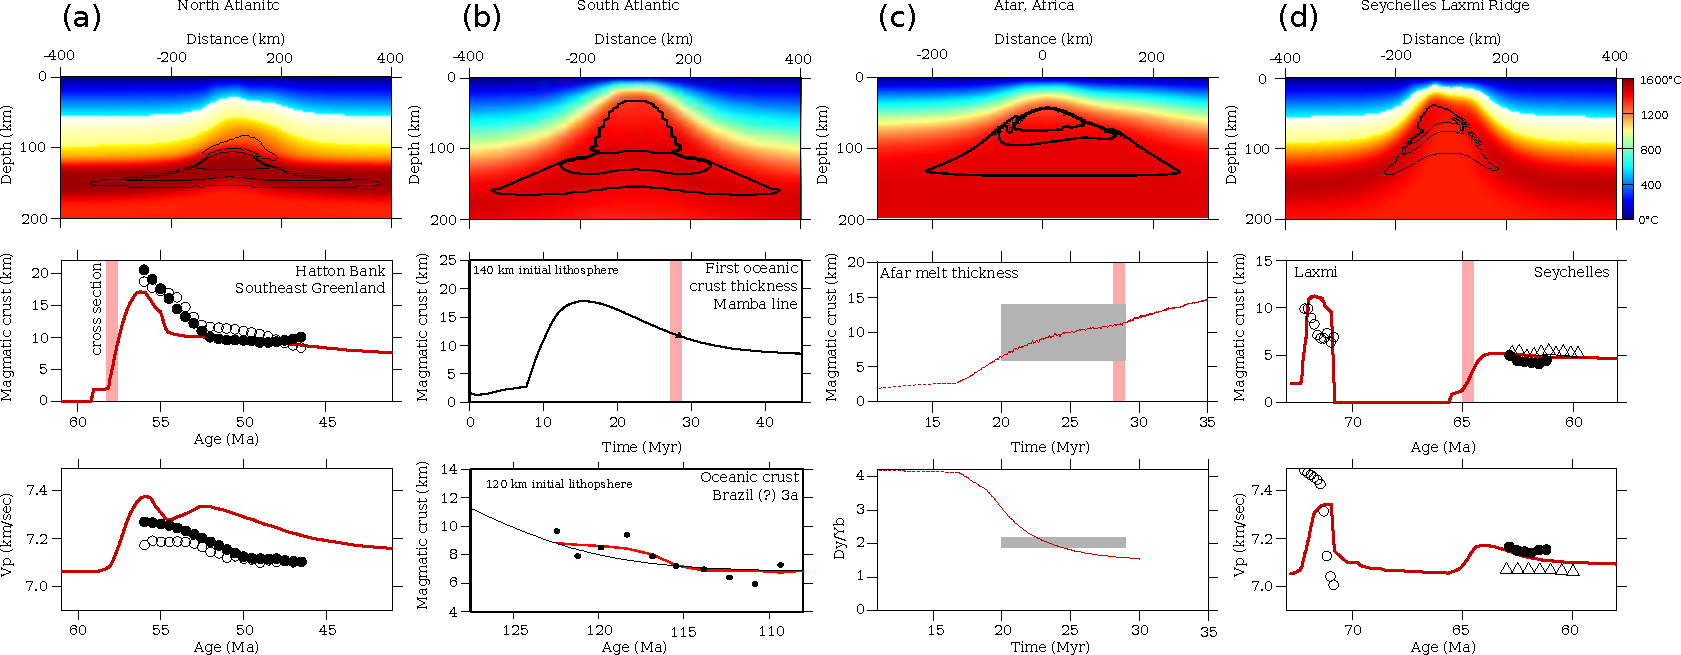
\includegraphics[width=22.5cm]{./figures/ch2-mantle2.pdf}
\caption{Key model results for four study areas \citep[see][]{armitage-2018}. The top figures show the thermal conditions within the model at the time step shown by the pink bar in the lower diagrams. The black outlines show the regions that are producing melt with contours representing 1\,\% (long dashed lines) and 2\,\% (short dashed lines) melting. The lower figures show examples of observations (symbols or in the Afar case a grey box) compared to model predictions (red lines). We have chosen to show models from early stage of rifting (North and South Atlantic) and from late stage (South Atlantic and Afar). In the former two examples there are rift jumps, hence the melt area shown is asymmetric. There is no other significance to the choice of time step for each location. (a) North Atlantic: the lithosphere has been pre-stretched by the formation of the Hatton Trough at $5\rm\,mm\,yr^{-1}$ \citep[see][]{armitage-etal-2009}, and subsequently the event that leads to break-up at a half spreading rate that is initially $40\rm\,mm\,yr^{-1}$ and reduces to $10\rm\,mm\,yr^{-1}$ at 55\,Ma. The model is compared to estimates of the thickness and $V_{p}$ of igneous intrusions from the SIGMA-3 -- iSIMM Hatton Bank conjugate margins \citep{hopper-etal-2003,white-etal-2008}. (b) South Atlantic: the lithosphere has been stretched in one phase at a half spreading rate of $14\rm\,mm\,yr^{-1}$ \citep[see][]{taposeea-etal-2016}. The model is compared to the thickness of the oceanic crust offshore Namibia (Mamba line) and Pelotas (ION-GX). (c) India–Seychelles: the lithosphere has been stretched in two phases, first the formation of the Gop Rift at a half spreading rate of $80\rm\,mm\,yr^{-1}$, followed by extension between the Seychelles and Laxmi Ridge at a half spreading rate of $60\rm\,mm\,yr^{-1}$ \citep[see][]{armitage-etal-g3-2011}. The model is compared to estimates of the thickness and P-wave seismic velocity ($V_{p}$) of igneous intrusions from both margins \citep{collier-etal-2009,minshull-etal-2008}. (d) Afar, Africa: the lithosphere has been stretched in two phases, first due to the formation of the southernmost Red Sea at $5\rm\,mm\,yr^{-1}$, and then within Afar at a half spreading rate of $7\rm\,mm\,yr^{-1}$ \citep[see][]{armitage-etal-2015}. The model is compared the estimates of the thickness of the igneous crust and the Dy/Yb ratio of melts erupted.}
\label{fg:4models}
\end{sidewaysfigure}

\begin{figure}
    \centering
    \includegraphics[width=12cm]{./figures/ch2-EAR.png}
    \caption{(a) The East African Rift region comprising the Afar region, the Main Ethiopian Rift (MER), and eastern and western branches (EB, WB) south of the study area (red box). Orange triangles represent Holocene volcanoes. Brown lines delineate active fault zones. (b) Horizontal slice at 500 km depth through the undamped P model, NEAR-P15. The black line indicates the orientation of the cross sections in (c) and (d). (c) Vertical cross section through the undamped NEAR-P15. (d) Vertical cross section through the undamped NEAR-S16. The cross section reveals two clusters of low-velocity anomalies below Afar and MER extending down to the base of the transition zone.}
    \label{fg:EAR}
\end{figure}

The seismic velocity found in inverse models of the mantle below the Northern East African Rift (EAR) is spectacularly low (Figure \ref{fg:EAR}). This coupled with the chemistry of lavas erupted would suggest that there is a source of very hot mantle below this young rift zone. Classic tomographic models of for Africa have suggested that there is a broad low-velocity layer present through the whole upper mantle beneath the EAR, and this is interpreted to be a large-scale upwelling named the African Superplume \citep[e.g.][]{ritsema-etal-1999}. As the number of seismometers deployed within Africa has increased the resolution of tomographic images has increased. It is now thought that this structure is potentially multiple smaller-scale features and not one large upwelling \citep{chang-2011,hammond-etal-2013,civiero-etal-2015,emry-etal-2019}. This complexity is not unique to the African structure, below Iceland the low-velocity anomaly is a complex branching structure \citep{rickers-etal-2013}, the Azores, Canary and Cape Verde low-velocity zones may be linked \citep{saki-etal-2015}, and likewise for structures below the Iberian peninsular and Maghreb \citep{civiero-etal-2018}. These interpretations lead to the suggestion that there exist secondary plumes rising below zones of active volcanism, as for example observed within laboratory experiments \citep{davaille-2005,kumagai-etal-2007}.

Secondary plumes, such as those within the experiments of \cite{kumagai-etal-2007}, arise due the stagnation of the main plume head. This is due to density changes in the mantle due to endothermic phase transitions at the 660\,km discontinuity \citep[e.g.][]{tosi-2011,bossmann-2013}. The stagnated material heats up the boundary at the 660\,km discontinuity and generates new plumes at a smaller scale, which would have a spacing of the order of hundreds of kilometers and leads to the hypothesis that the structures seen in the inverse models from seismic arrivals are due to such small-scale plumes \citep{civiero-etal-2015}. In collaboration with Chiara Civiero and Saskia Goes, we tested this hypothesis. The goal was to use a similar approach to earlier work on the EAR and the East Pacific Rise \citep{armitage-etal-2015,goes-etal-2012}:
\begin{itemize}
\item[1] Develop a forward model of the geodynamic processes. In this case we wanted to model Rayleigh Bérnard convection and the destbilisation of hot material, Rayleigh Taylor instabilites, in three dimensions at a scale similar to the EAR.
\item[2] Convert the physical model properties to seismic velocities, taking into account the effects of attenuation.
\item[3] Resolve the numerical model at the same resolution as the tomographic models. This means using the numerical model as an input model for the inversion and observing how the high resolution image gets damped and smoothed due to the resolution of the seismic array.
\end{itemize}

\begin{figure}
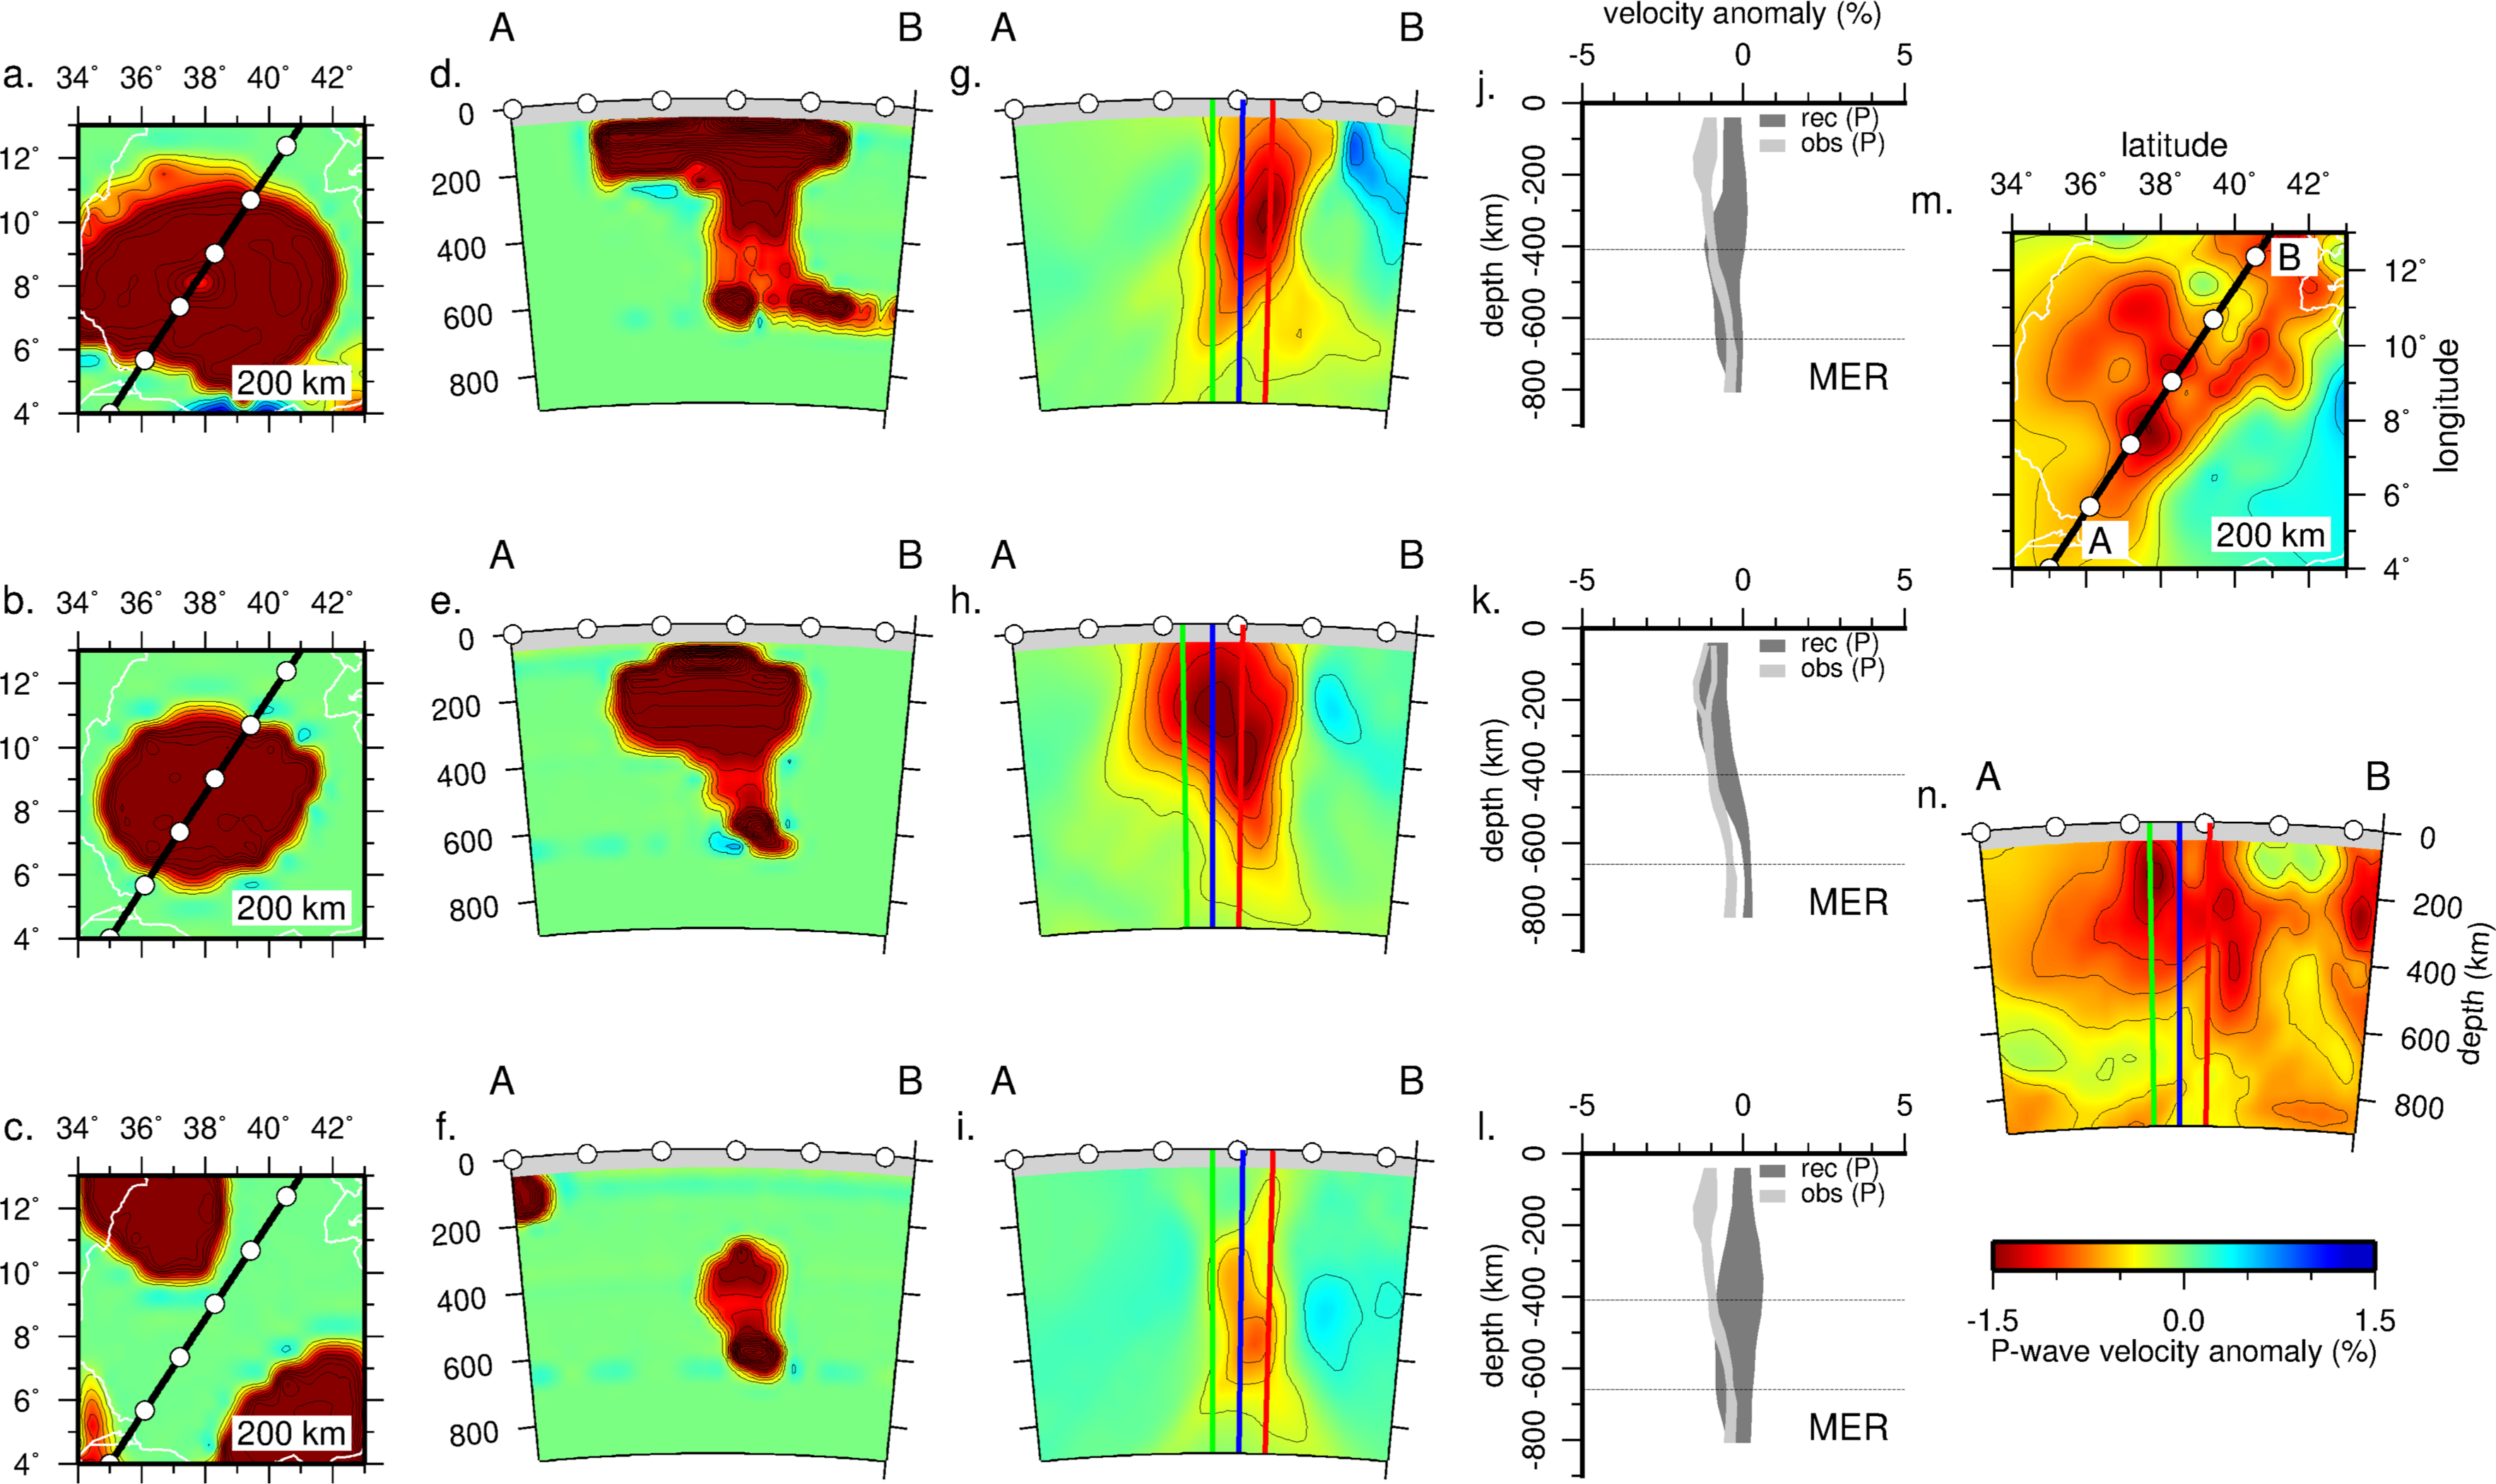
\includegraphics[width=\textwidth]{./figures/ch2-tomography.png}
\caption{Figure from \cite{civiero-etal-2019}: Horizontal slices and vertical cross sections through the P wave from the destabilisation of a layer with an excess temperature of $200\rm\,^{\circ}C$ (Rayleigh Taylor instability), focused below the Main Ethiopian Rift. The orientation of the cross sections (black line) is shown in each 200 km depth slice. (a–c) Horizontal slices at 200 km depth through the synthetic models of LS (a), MS (b), and ES (c) phases. (d, g) Synthetic and resolved images of the LS plume phase; (e, h) synthetic and resolved images of the MS plume phase; (f, i) synthetic and resolved images of the ES plume phase. The resolved LS plume (g) lost its head due to the lack of resolution at shallow upper-mantle depths. The MS phase (h) is well resolved because the head of the input model (b) is relatively strong and laterally confined. Although some smearing, the ES structure (i) is quite well
recovered. (j–l) Input and retrieved P wave velocity anomaly envelopes (\%) along the green, blue, and red profiles drawn in the cross sections. Within the transition zone the retrieved and observed velocity anomalies of the MS and LS plumes overlap. (m) The 200 km depth slice through the NEAR-P15 model. (n)
Vertical cross section through the NEAR-P15 model. The spacing between the contours is 0.25\,\%. White points indicate the distance every $2\rm\,^{\circ}$ . The color scale is the same for all the panels.}
\label{fg:EAR-plumes}
\end{figure}

We explored two possabilities, first that the small-scale plumes are like Rayleigh Bérnard convection cells and secondly that they are due to the destabilisation of ponded plume material (Rayleigh Taylor instabilites). In total 10 model setups were explored with additional variations to the assumed mantle rheology, initial thermal strucutre and boundary conditions, and model aspect ratio (see \citealp{civiero-etal-2019} for the full details). By converting the numerical model to synthetic tomographyic images it was quickly found that the thermal structure of the small-scale plumes had to create a significant and sharp contrast in seismic velocity. Simple Rayleigh Bérnard convection lead to plumes that were either too thin (for a non-Newtonian rheology) or were too diffuse (for a Newtonian rheology), such that the synthetic tomography does not recover the strong contrast in seismic velocity seen in the inversions \citep{civiero-etal-2018}.

The only models that could recreate the contrast in seismic velocity within the inversions were those that looked at the Rayleigh Taylor-like destabilisation of a layer of hot material that was initially at the base of the model domain at between 600 and 700\,km (Figure \ref{fg:EAR-plumes}). This layer rises upwards as plume-like structures with a spacing that is similar to the the spacing in the tomographic models (Figure \ref{fg:EAR-plumes}). The implication is that below the EAR mantle material stagnated below the 660\,km discontinuity due to mineral phase changes. Rather than this ponded material heating the upper mantle and creating secondary plumes, the ponded material became buoyant and rose into the upper mantle as a Rayleigh Taylor instability giving rise to the distribution of volcanism we observe today in the EAR. One mechanism that could lead to such behaviour is internal heating, which would cause a stagnated plume head to become thermally buoyant over time and destabilise.

One important point that comes from this work is that the simplistic interpretation of the patterns seen in the seismic tomography as being due to small-scale plumes is overly simplistic. There is a need to go further and explore if such interpretations are possible. Secondary plumes due to a thermal boundary layer at the 660\,km discontinuity cannot create the observed magnitudes of low velocities. This is important because it means that material passes through the boundary between the upper and lower mantle. Beyond trying to understand how the deep Earth functions, this research has wider implications to how we practice science. The interpretation of an inverse model is not an observation nor a result. Seismological studies should not end with an interpretation of the preferred inversion. Rather, these interpretations should be posed as hypotheses that can be tested. We can resolve numerical models at the resolution of seismic deployments \citep[e.g.][]{goes-etal-2012,civiero-etal-2019}, and by doing so discover if the hypothesis stack up against the seismic data.

At a shallower scale, from an inverse model based on receiver functions and Rayleigh waves, it was interpreted that the crust and mantle lithosphere are decoupled below the Main Ethiopian Rift \citep{keranen-etal-2009}. It was thought that the seismic velocities are indicative of a hot and therefore weak lower lithosphere. Narrow rifting in the Main Ethiopian Rift was therefor due to pre-existing structural controls in the crust and not due to the integrated strength of the lithosphere \citep{keranen-etal-2009}. However, the width of the region of extension has been shown, numerically, to depend on the rhoelogical laws chosen for the crust and lithosphere \citep[e.g.][]{buck-1991,brun-1999,brune-etal-2017}. Furthermore, the timing of the onset of volcanism is affected by the crustal strength within numerical models \citep{ros-etal-2017}. Therefore, it is possible that the structure of early rifting in the northern East African Rift is due to crustal rheology rather than an unknown inheritance. Importantly, the interpretation from the seismic data can be treated as a hypothesis and tested using numerical models of our best understanding of the physics behind the deformation of the upper mantle.

In collaboration with Kenni Petersen, we developed a 2D model of visco-elasto-plastic deformation of the upper mantle (MESS\footnote{MESS: Multigrid Elastic and Stuff Solver (or Multigrid Elasto-plastic-viscous Strain Solver), see \url{https://bitbucket.org/johnjarmitage/mess}}) that includes melting and in particular the prediction of melt composition \citep{petersen-etal-2015,armitage-etal-g3-2018}. By varying the strength of the crust we showed that evolution of the depletion of lavas in light trace elements is a function of the strength of the crust. When the crust is strong, it thins rapidly and extension localises creating a narrow rift. This is analogous to there being only a thin lithospheric lid on top of the zone of partial melting. This thin lid does not suppress the development of a `triangular' zone of partial melting (as shown in Figures \ref{fg:melt-region} and \ref{fg:4models}). The result is that light trace elements, such as lanthanum (La), are depleted rapidly with respect to heavier trace elements, such as ytterbium (Yb). If however the crust is weak, extension is not localised and a thicker lithospheric lid rests upon the zone of partial melting. This results in a slower reduction in light relative to heavy trace elements within the erupted lava \citep{armitage-etal-g3-2018}.

\begin{figure}
\centering
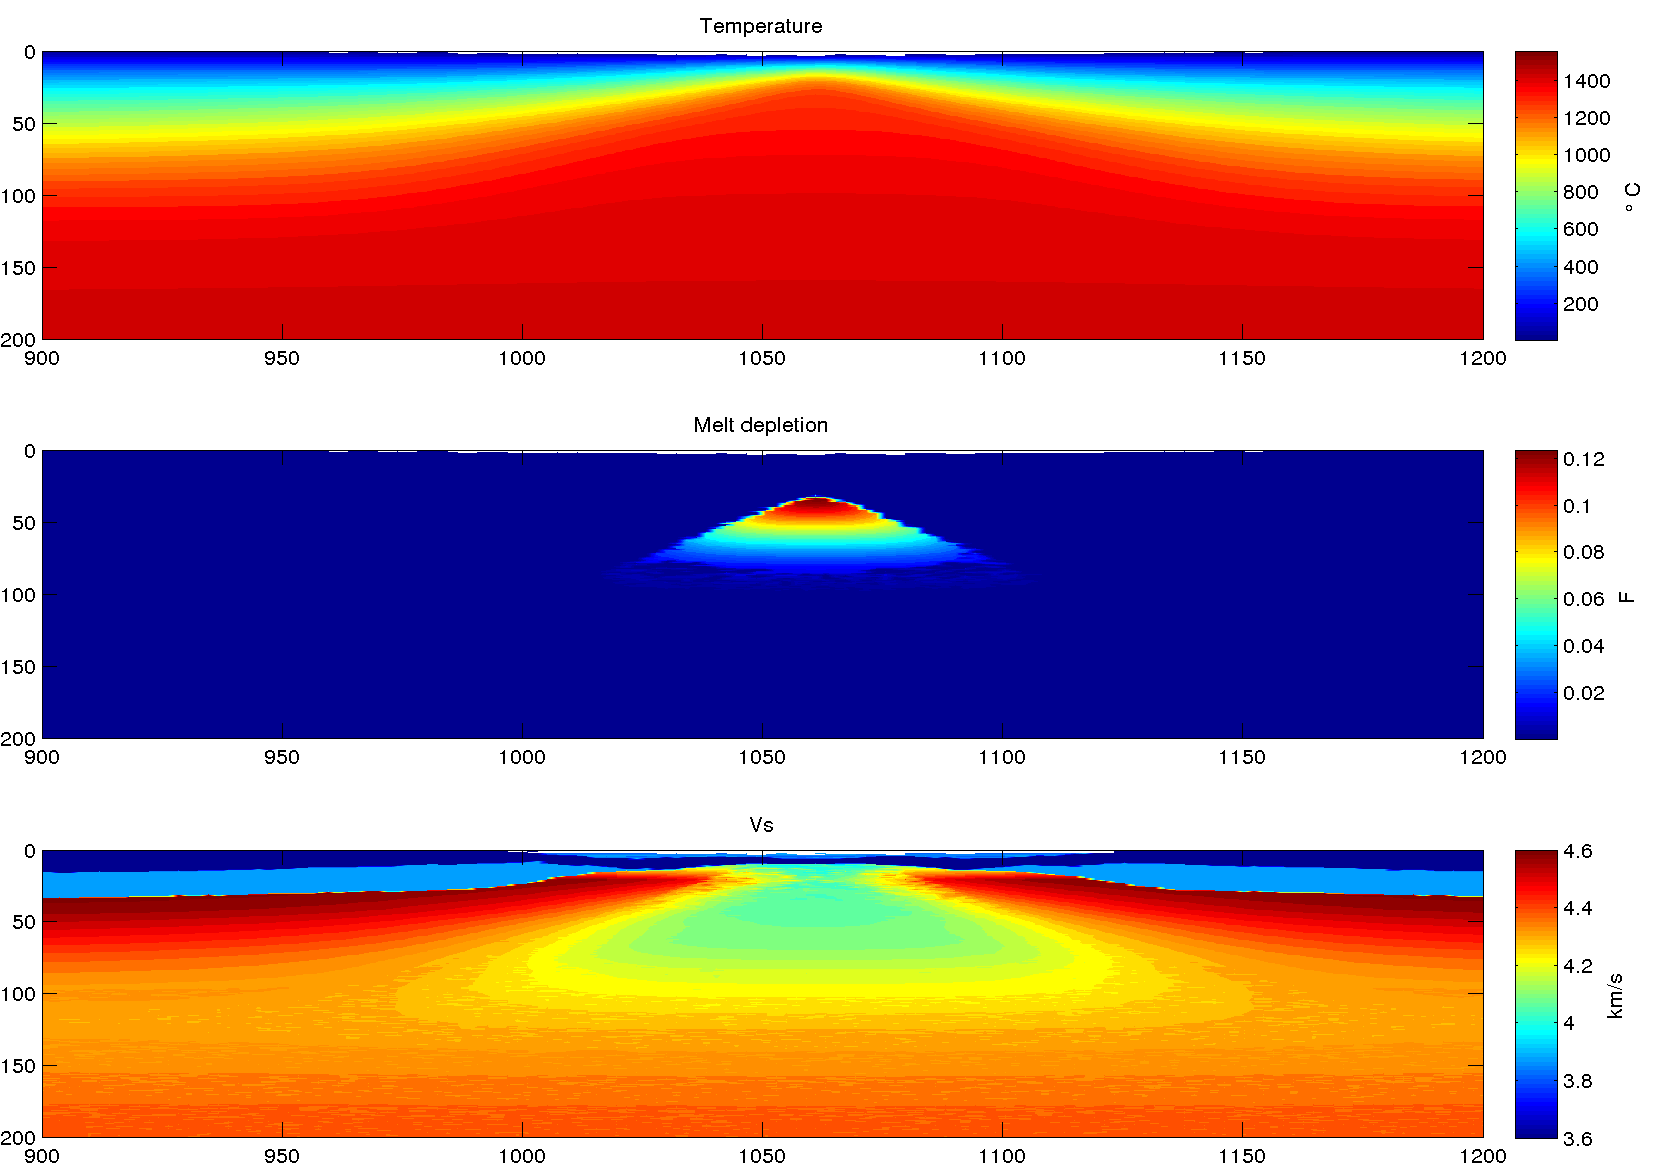
\includegraphics[width=\textwidth]{./figures/ch2-mantleVs.pdf}
\caption{Predicted thermal structure, melt depletion, and S-wave seismic velocity after 25 Myr of extension for with an extension rate of $5\rm\,mm\,yr{-1}$ and mantle potential temperature of $1350\rm\,^{\circ}C$. (a) Temperature, (b) melt fraction, and (c) S-wave seismic velocity. Figure taken from \cite{armitage-etal-g3-2018}.}
\label{fg:mantleVs}
\end{figure} 

When this model was applied to the Main Ethiopian Rift it was found that in order to recreate the observed lava chemistry, only a model with a strong crust could achieve sufficient melt generation. Furthermore, when the predicted upper mantle structure was converted to S-wave velocity (Figure \ref{fg:mantleVs}), it was found that the model velocities were within the range of the observed 1D inversions (Figure \ref{fg:MER-Vs} black line). The hypothesis that breakup in the Main Ethiopian Rift is defined by the extension of a weak lithosphere does not match the observations \citep[c.f.][]{keranen-etal-2009}. The numerical model that best fits the data is of a strong lithosphere. This demonstrates that hypotheses, or \emph{interpretations}, based from inverse seismic models can be tested with forward numerical models.

For shallower depths the forward model does not match the low seismic velocities required by the inversion (Figure \ref{fg:mantleVs}). However, if it is assumed that 1\,\% melt is stored within the lithosphere above a depth of 40\,km, then the shallow structure can be even better explained. The 2D code MESS does not include melt transport (e.g. equation \ref{eq:mass-melt}) and therefore the hypothesis that there is significant melt storage within the uppermost lithosphere below the Main Ethiopian Rift was not explored. However, as developed in the following section, this aspect could be incorporated in future studies.

\begin{figure}
\centering
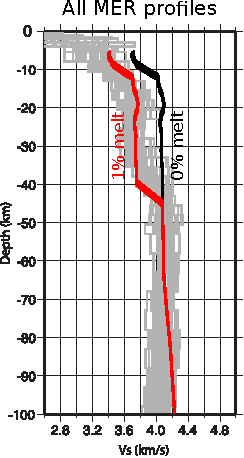
\includegraphics[width=4cm]{./figures/ch2-MER-Vs.pdf}
\caption{Comparison of the predicted S-wave seismic velocity from the for-ward model with a strong lower crust (Figure \ref{fg:mantleVs}c), and the ensemble vertical profiles from the joint inversion of Rayleigh waves and receiver functions below the Main Ethiopian Rift \citep{keranen-etal-2009}. The black line is the model $V_{S}$ assuming no melt storage, the red line assumes that 1\,\% melt is stored above 40\,km depth.}
\label{fg:MER-Vs}
\end{figure}

\subsection{Iceland}

\begin{figure}
\centering
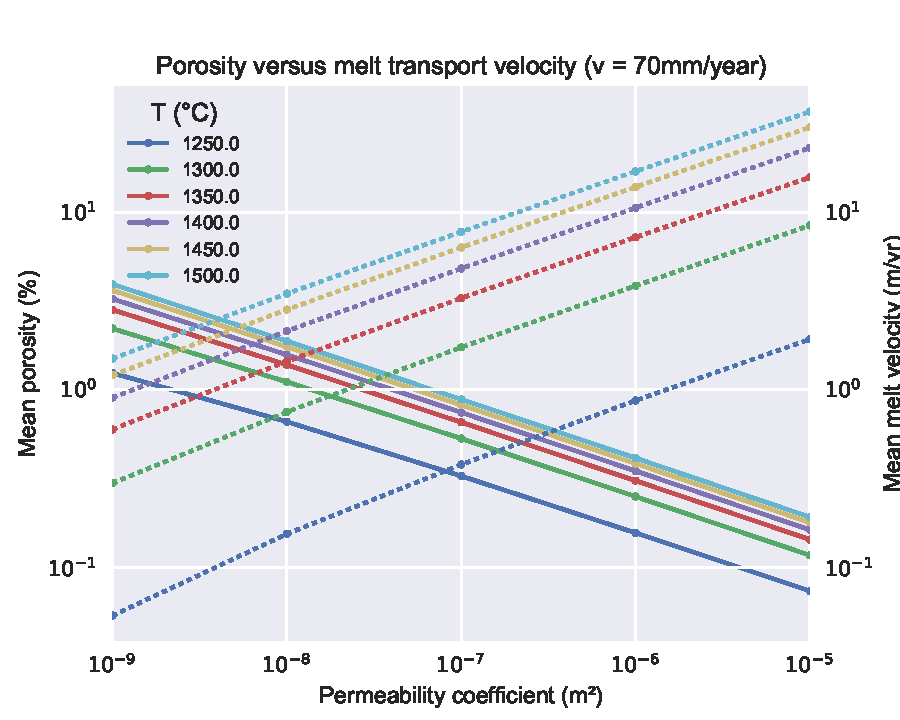
\includegraphics[width=8.6cm]{figures/ch2-phi-vm.pdf}
\caption{Logarithmic plot of the variation in modelled porosity (solid) and melt flow velocity (dashed) with permeability coefficient and temperature, with up-welling velocity constant at $70\rm\,mm\,yr^{-1}$. The relationship between porosity and mean melt flow velocity is inversely proportional as a function of the permeability coefficient, and proportional as a function of temperature. Figure is from \cite{franken-etal-2020}.}
\label{fg:phi-vm}
\end{figure}

The retention of melt within the upper mantle, as invoked at the end of the last section, has been cited as causing seismic discontinuities and regions of low velocity observed below volcanic islands, rift zones, and mid-ocean ridges \citep[e.g.][]{forsyth-etal-1998,harmon-etal-2009,rychert-etal-2012,rychert-etal-2014}. Typical estimates of the quantity of melt range from 0.1\,\% to 2\,\%. The low seismic velocities below Iceland can be explained by the presence of high temperatures but discontinuities required by receiver function inversions would require an extra $\sim 1$\,\% melt \citep{rychert-etal-2018}. High melt retention would naturally imply low melt velocities and low permeability (Figure \ref{fg:phi-vm}; \citealp{weatherley-2016,franken-etal-2020}). However, forward modelling of decompression melting below both the East Pacific Rise and Afar (Figure \ref{fg:4models}c; \citealp{goes-etal-2012,armitage-etal-2015}), suggest that high melt retention, $>0.5$\,\% is unlikely. 

The glaciers on Iceland have been reducing in size since the last glacial maximum. Iceland experienced a rapid deglaciation around ten thousand years ago (Figure \ref{fg:iceland-map}). The rapid depressurisation of the upper mantle due to this loss in surface load could lead to an significant increase in decompression melting \citep{jull-1996}. This is in line with outcrop evidence of the volume and composition of lava erupted since the late-Pleistocene \citep{maclennan-etal-2002,sinton-etal-2005,eksinchol-etal-2019}. However, if the observed change in lava composition and volume estimates were caused by deglaciation, the transport of melt from the zone of partial melting to the surface must be rapid, and rapid melt transport implies low melt retention (Figure \ref{fg:phi-vm}). This is therefore again at odds with the interpretation of high melt retention derived from seismic inversions.

\begin{figure}
\centering
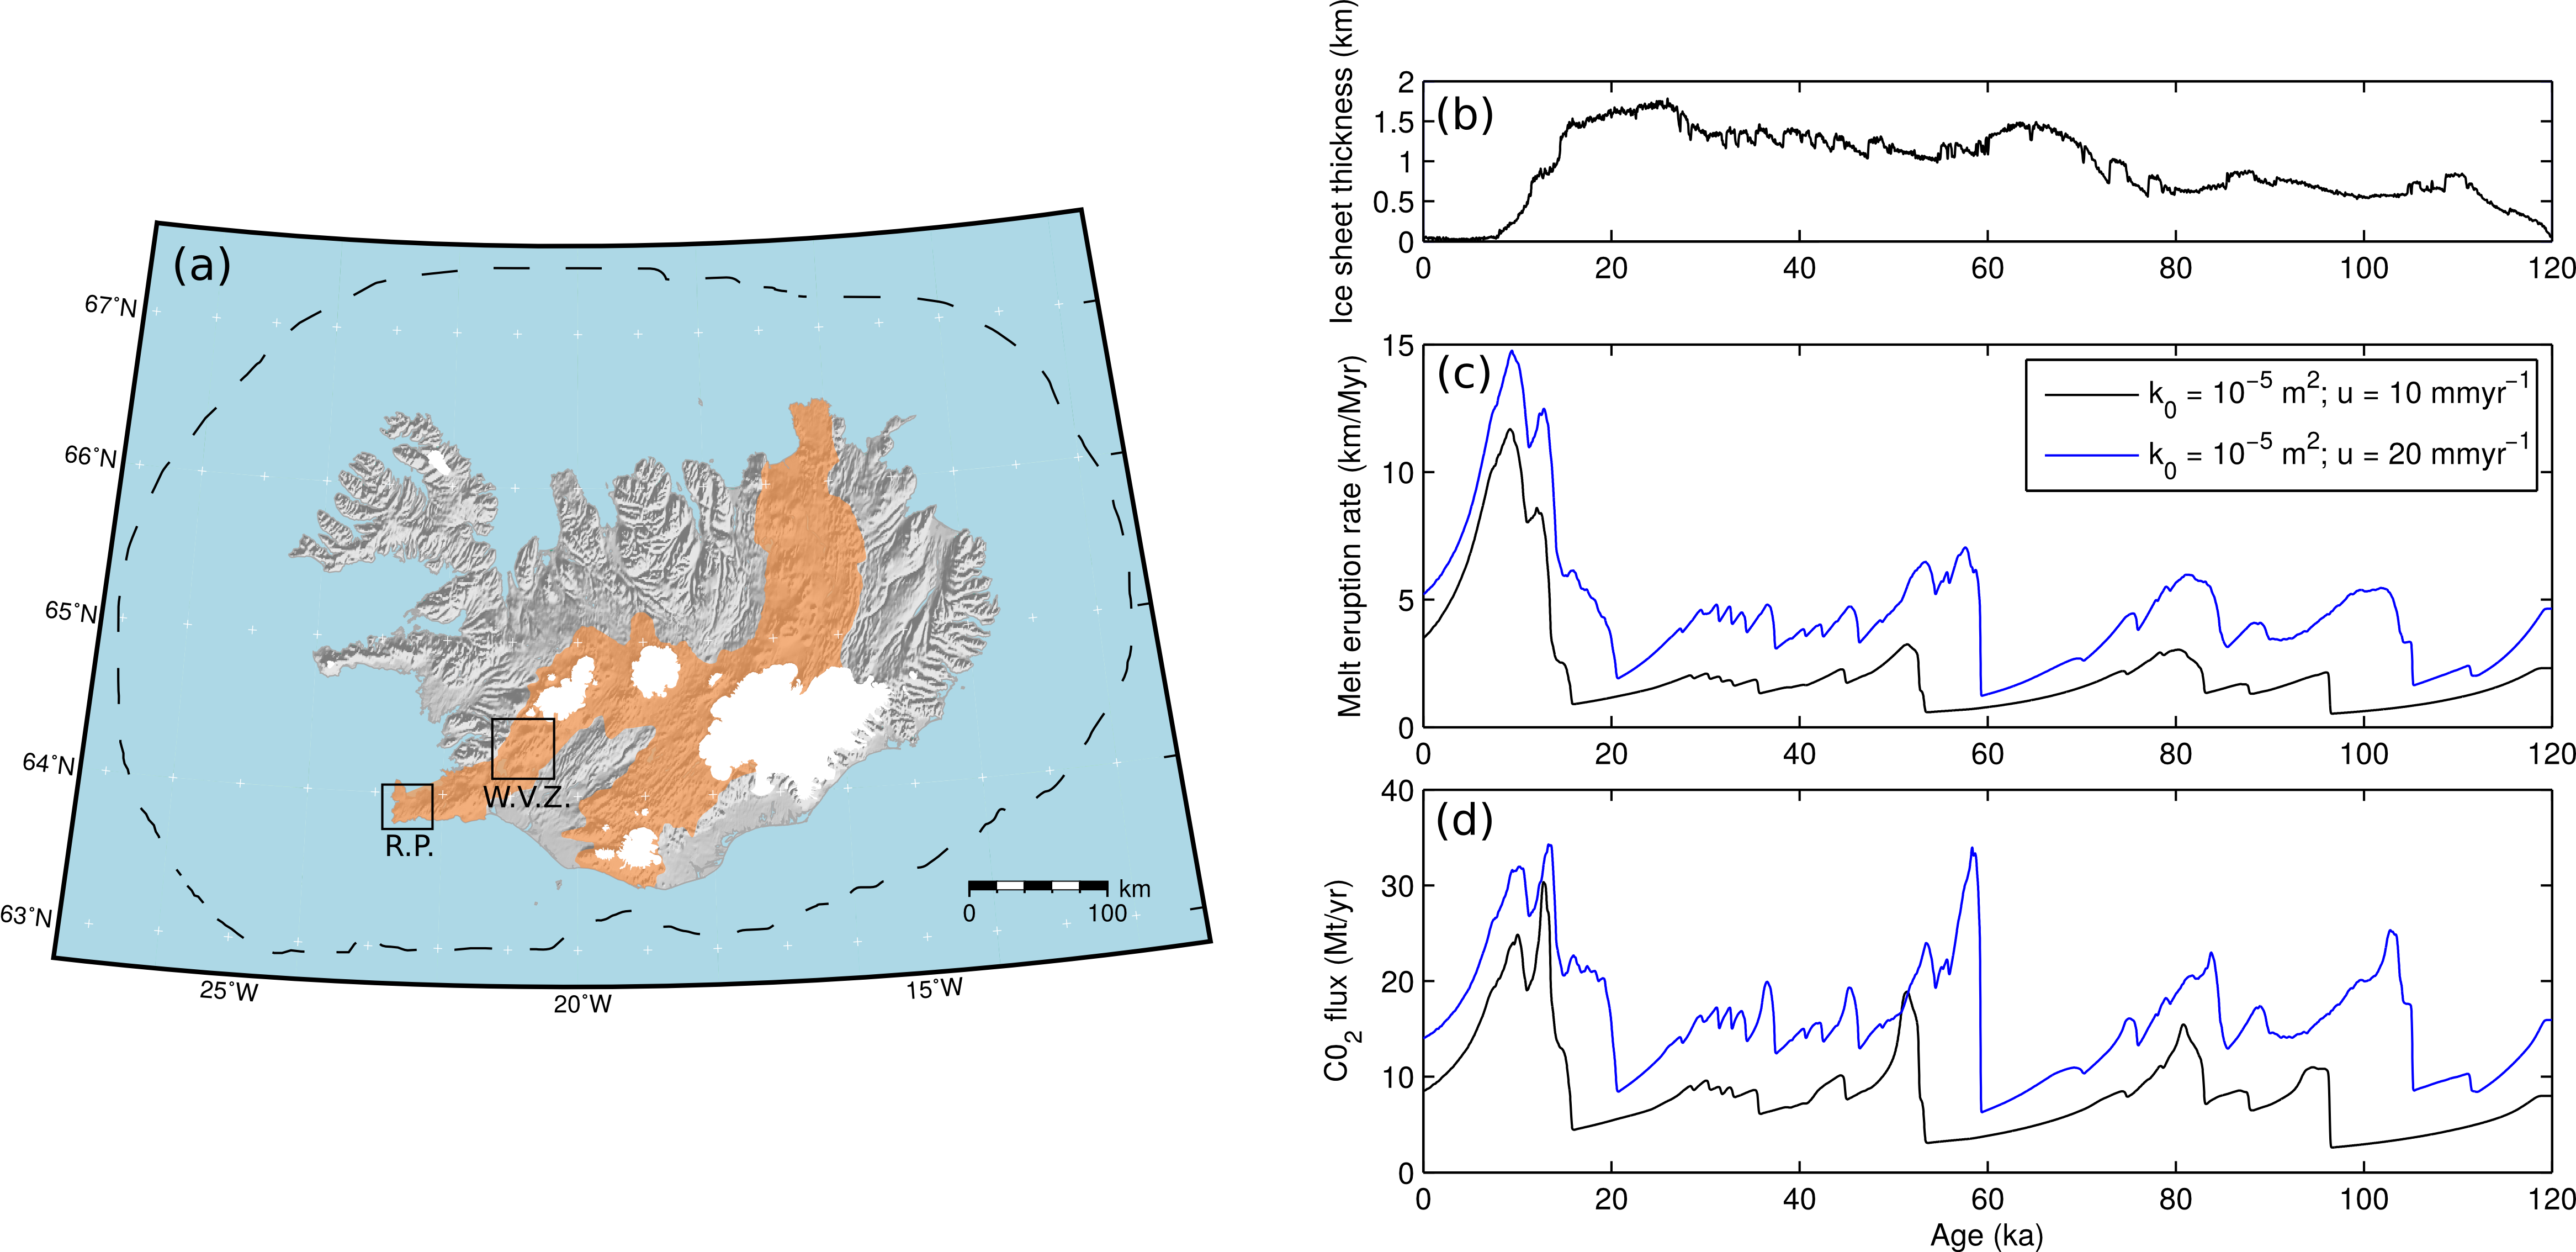
\includegraphics[width=\textwidth]{./figures/ch2-iceland-map.png}
\caption{Response of the model to periodic and observed ice sheet thickness changes of the last 120\,ka. (a) Map of Iceland showing the locations of the volcanic rift zones in orange and the maximum extent of the ice sheet at the last glacial maximum (dashed line). The boxes show the location of the Reykjanes Peninsular (R. P.) and the Western Volcanic Zone (W. V. Z.). (b) The ice sheet thickness predicted from the ice sheet model M1 over the last 120\,ka. (c) Melt eruption rate and (d) carbon flux response to the step change in ice sheet thickness: black line, an upper mantle permeability coefficient of $k_{0} = 10^{-5}\rm\,m^{2}$ and up-welling velocity of $10\rm\,mm\,yr^{-1}$, and blue line, an up-welling velocity of $20\rm\,mm\,yr^{-1}$.}
\label{fg:iceland-map}
\end{figure}

To understand if the observed change in lava composition is due to deglaciation I worked with Kenni Petersen, David Freguson, and Tim Creyts, to create a 120\,kyr history of ice sheet growth and decay on Iceland (Figure \ref{fg:iceland-map}b) and develop a 1D model\footnote{The 1D model can be found at: \url{https://bitbucket.com/johnjarmitage/melt1d-icesheet/}} that can predict eruption rates, lava compositions, and melt retention as the surface load changes \citep{armitage-etal-grl-2019}. From exploring the physically plausible parameter space, we found that deglaciation would indeed impact lava eruption rates if the mantle permeability is high (Figure \ref{fg:iceland-map}c and d). In order to recover a system response that matched the estimated eruption rates from outcrops, and the observed neodymium (Nd) concentrations the permeability of the mantle $k_{\phi} = k_{0}\phi$ needs to be on the order of $10^{-14}\rm\,m^{-2}$, melt retention of $\sim 0.1$\,\% \citep{armitage-etal-grl-2019}.

This model result has implications for volcanic CO$_{2}$ degassing post deglaciation, that I will not go into detail on here \citep[see][]{armitage-etal-grl-2019}. The model result also has implications for assumptions of melt retention within the upper mantle. As stated above, low seismic wave speed anomalies within the mantle, inferred from inverse models, are often interpreted to be due to high melt retention within the mantle. This, I have demonstrated, is not possible if we also simultaneously have a mantle melting system that responds rapidly to deglaciation, and potentially sea level change \citep{huybers-2009}. Therefore, we need to change our interpretations and think harder as to why inverse models suggest sharp mantle seismic discontinuities and low velocities below regions of volcanism.

\subsection{La Réunion}

\begin{figure}
\centering
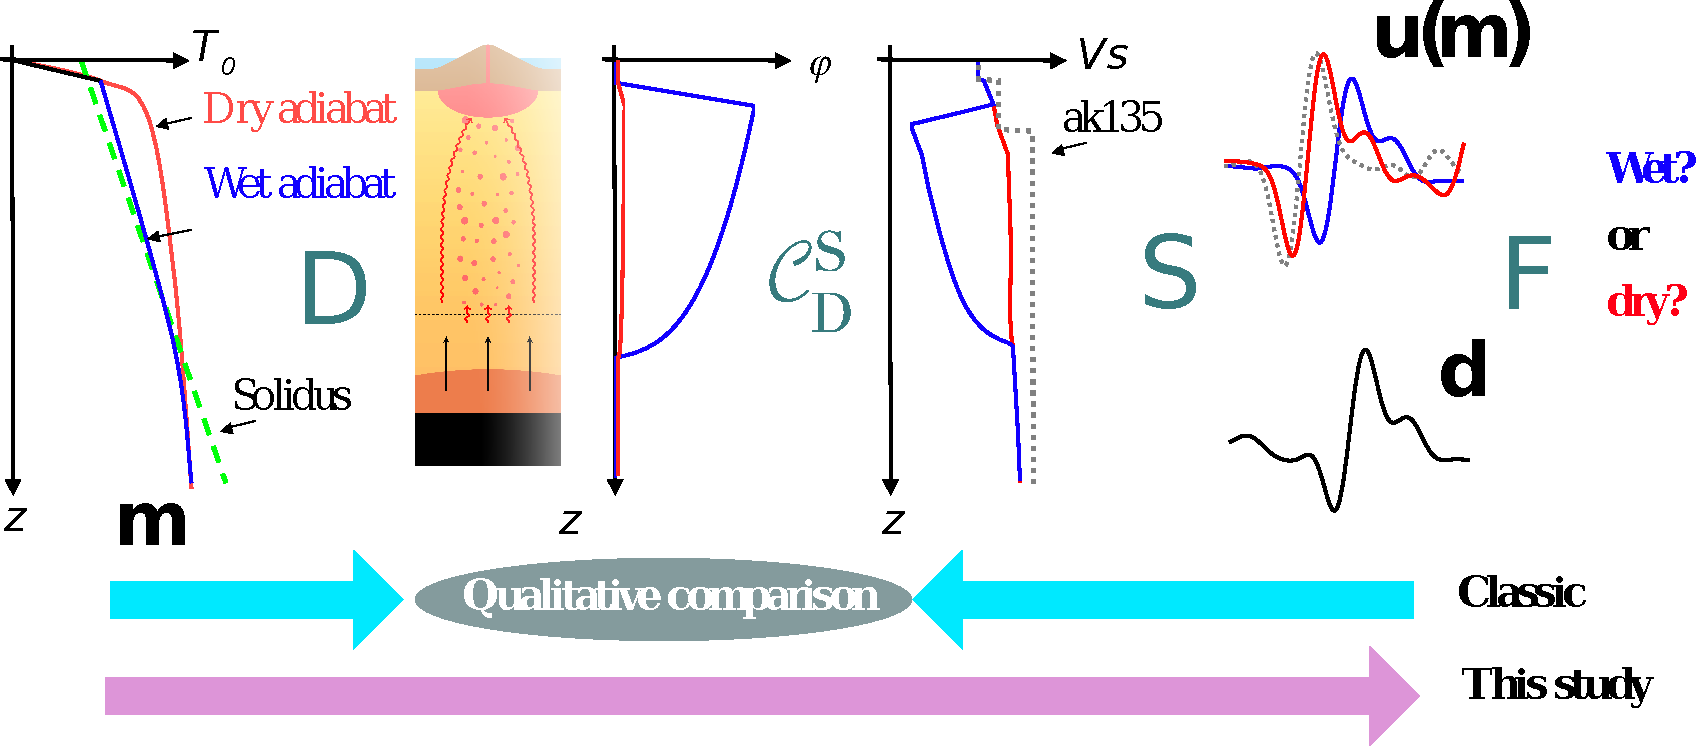
\includegraphics[width=\textwidth]{figures/ch2-schema.pdf}
\caption{Conceptual schema of the waveform seismic filtering strategy \citep[see][]{franken-etal-2020}. On the top from the left to right: we first generate ($\mathcal{D}$)  geodynamical scenarios with different initial conditions $\mathbf{m}$ ($T_0$ for example: wet and dry in blue and red, respectively) in order to obtain a steady-state snapshot (vertical variation of porosity $\phi$ for example). We then translate  ($\mathcal{C}_\mathrm{D}^\mathrm{S}$) the set of geodynamical parameters such as $\phi$ to a set of seismological parameters such as $V_S$. We then generate ($\mathcal{S}$) seismic waveforms $\mathbf{u}$ to look for the sensitivity of $\mathbf{u}$ with respect to $\mathbf{m}$. We define a filter $\mathcal{F}$ that can distinguish the different scenarios $\mathbf{m}$: we then analyse the observed data $\mathbf{d}$ to conclude the preferred geodynamical scenario. Classical approaches try to fit the intermediate parameter sets such as seismic velocity structure or porosity structure that has unknown error bars due to a series of inversion procedures.}
\label{fg:inversion}
\end{figure}

In the last four years I tried to push beyond the classic interpretation of inverse models that dominates Earth science and seismology in particular. Rather than creating methods to compare synthetic seismic structures with the inverted structures, I wanted to use the forward model to simulate the true observation: the seismic waveform recorded at the receiver (Figure \ref{fg:inversion}). In collaboration with Thijs Franken, Nobu Fuji, and Alexandre Fournier we focused on melt migration and how partial melt might impact seismic arrivals at La Réunion.  A strong low velocity region is imaged in tomographic models below La Réunion \citep{mazzullo-etal-2017}, and we could be tempted to assume it is due to high melt retention. However, by creating a 1D forward model of melt production and retention we can propagate numerically a seismic wave through this 1D system. The arrival can then be compared to the observed waveforms, to try and find a best fit. This approach is more fully described in the PhD thesis of Thijs Franken, in \cite{franken-etal-2020}, and is summarised in Figure \ref{fg:inversion}.

We ran models through the full parameter space for 1D melting and melt transport, and found that only a select few models could match the travel time difference and the S-to-P travel time differential when synthetic waveforms were compared to the observations at the RER Geoscope permanent station. These few models implied either high melt retention (low porosity) and cold mantle temperature ($\sim 1250\rm\,^{\circ}C$), or low melt retention (high porosity) and hot mantle temperature ($\sim 1450\rm\,^{\circ}C$). The best fit model would suggest conditions below La Réunion of melt retention of $<$0.28\% and high melt extraction rates of 8.37-18.35 $\rm\,m\,yr^{-1}$ \citep{franken-etal-2020}. Which would imply a melting system that can react rapidly, geologically speaking, to change. More recently a similar model of melt generation and transport was used to explore rates of melt transport beneath Iceland \citep{jones-2020}. Here it was found that in order to match the observed change in volumes of melt erupted melt would have to travel at roughly $30\rm\,m\,yr^{-1}$. The combined estimates of melt extraction rates from Iceland and Réunion would suggest that melt retention is low.

At the beginning of this chapter I introduced the hypothesis based on inverse seismic models that large quantities of melt are retained beneath regions of volcanism. This hypothesis is based in the interpretation that low seismic velocity anomalies can only be explained by lenses of melt reducing the speed at which seismic waves can travel. This hypothesis can be tested, and in doing so it is clear that melt is unlikely to be the cause of low velocity zones. Rather it is the combined effect of thermal attenuation and significantly smaller quantities of melt that create the travel time delays and changes in the observed waveforms \citep{franken-etal-2020}. Hopefully in the future, seismological research will continue to move beyond the simple interpretation and start to test the hypothesis behind the interpretation.

\section{Surface Processes}

The surface of the Earth contains the most time-sensitive record of the past. Accumulations of sediment can give information about change in climate, tectonics and even the mantle throughout geological time. However, as with the fields of seismology and geochemistry, the observations require interpretation to extrapolate how physical processes have impacted the geological record. As with melt generation and transport, sediments are created and transported to create the final observation: a stratigraphic section. Over the last decade I have developed numerical models to try and predict observations of grain size change in stratigraphic units (see Appendix \ref{subsec:a-simplified-model-of-surface-processes}; \citealp{armitage-etal-ngeo-2011,armitage-etal-2015,armitage-etal-br-2018,armitage-2019}). In this section I will then describe two regions where I have used these models to try and understand what caused the observed sediment deposition: the Eocene Escanilla system in Spain and the Book Cliffs in central USA (the articles for these two examples are included within Annex B).

\subsection{Eocene Escanilla sedimentary system, Spain}

\begin{figure}
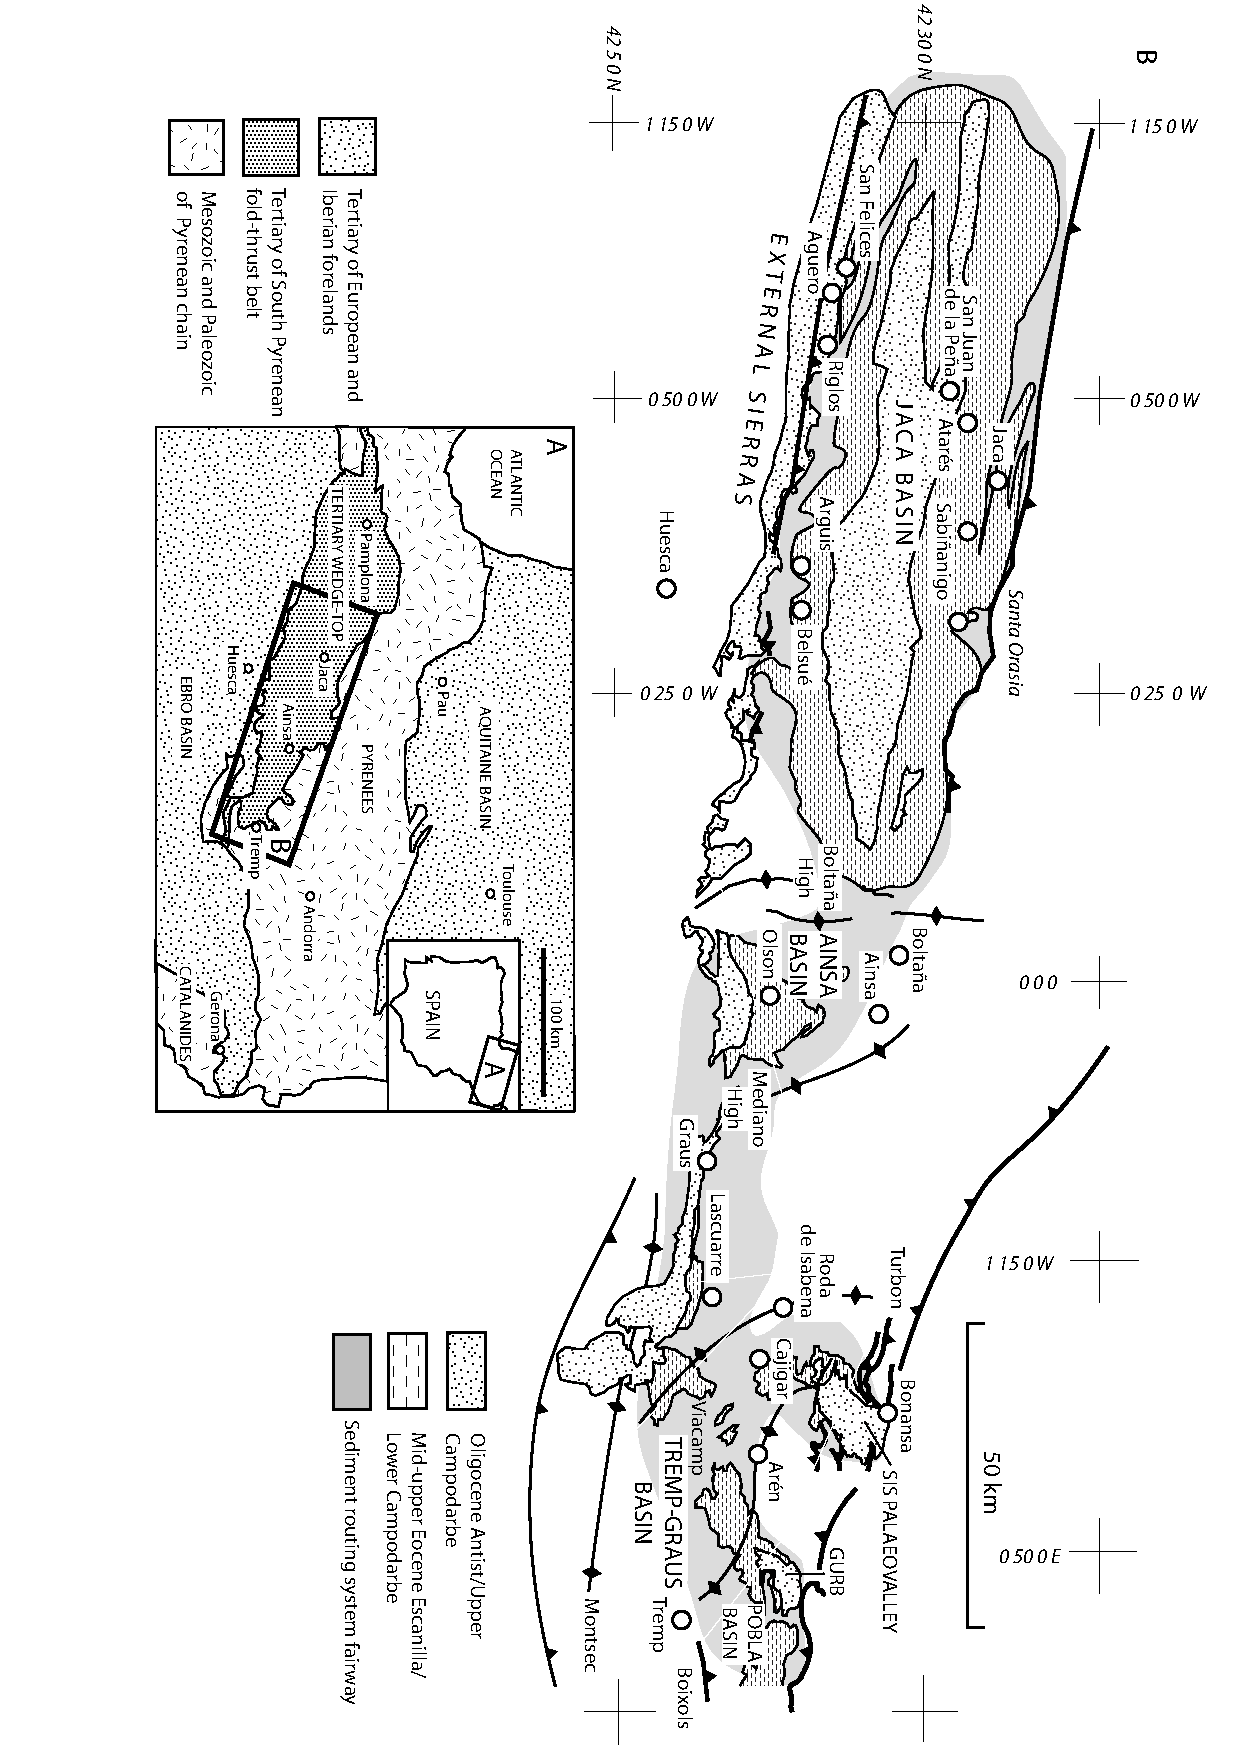
\includegraphics[height=\textwidth,angle=90]{./figures/ch2-escanilla-map.pdf}
\caption{A) Location of the Escanilla paleo--sediment-routing system in the Tertiary wedge top of the south-central Pyrenees, northern Spain. B) Detail of the Escanilla paleo--sediment-routing system fairway, after \cite{michael-etal-2014a}.}
\label{fg:escanilla-map}
\end{figure}

The Escanilla sediment-routing system has its source regions in the south-central Pyrnean orogen (Figure\ref{fg:escanilla-map}). Sediment was transported throughout the Lutetian to Priabonian (41.6 to 33.9\,Ma) from wedge top basins in the east to marine deposits in the west. It can be simplified into two major source regions that fed sediment into the Sis Paleaovalley and Pobla Basin (Figure\ref{fg:escanilla-map}). The sediment fairway can then be simplified to a single depositional cross section that extends from the Gurb-Pobla and Sis depocenters through the Tremp-Graus, Ainsa, and Jaca basins (Figure \ref{fg:escanilla-map}; \citep{michael-etal-2013}). The position of the limit of gravel deposition, the gravel front, and sand deposition, the sand front, for three time periods were measured by Nicolas Michael and Philip Allen \citep{michael-etal-2013}. It was found that the gravel front migrated westwards significantly in the final time period, from 36.5 to 33.9\,Ma. A classic interpretation of this progradation would be that there was increased precipitation within this third time period, which lead to increased energy within the system and the migration of the gravel front towards the west.

\begin{figure}
\centering
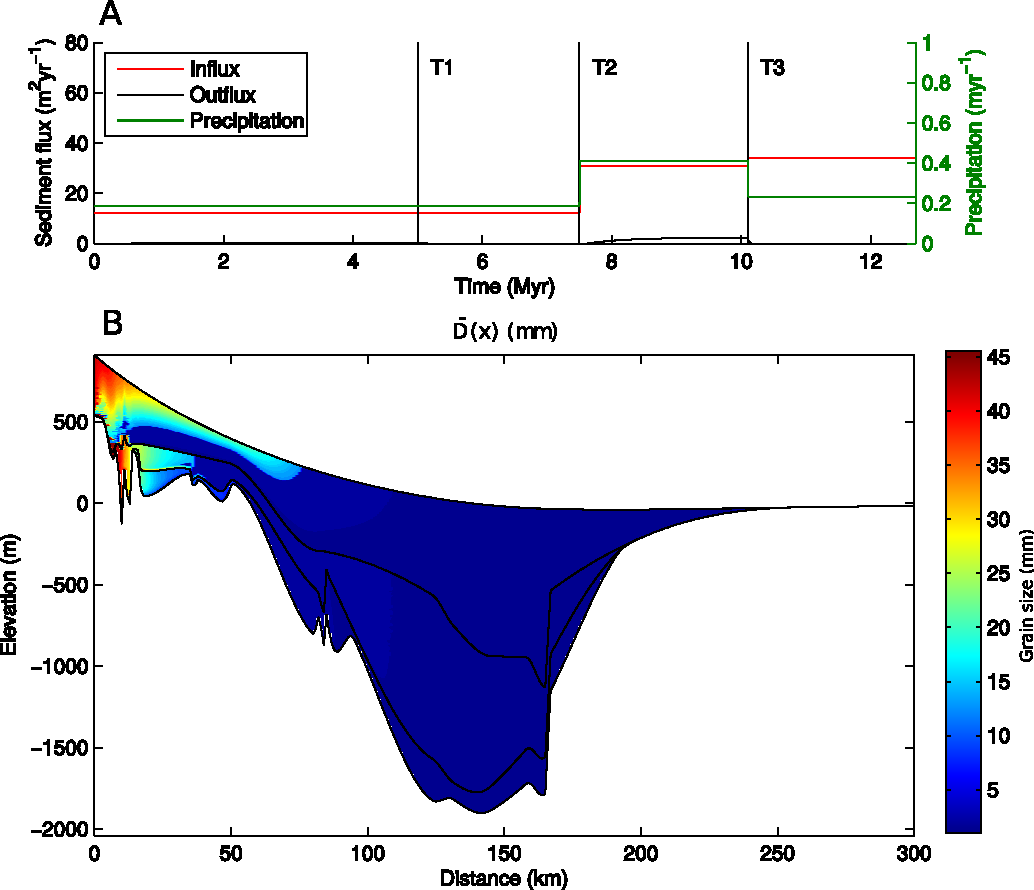
\includegraphics[width=8.6cm]{./figures/ch2-escanilla-model.pdf}
\caption{Stratigraphic architecture predicted by the forward model run that most closely matches the observed location of the gravel front. A) Sediment flux in and out of the basin and precipitation rate against time. B) Distribution of grain-size deposited in the idealized Escanilla paleo--sediment-routing system.}
\label{fg:escanilla-model}
\end{figure}

By using the 1D model for sediment transport, combined with grain-size fining, a Monte-Carlo--like simulation was run to find the combination of change in surface run-off and catchment erosion that could match the position of the gravel and sand fronts within the system \citep{armitage-etal-2015}. The best fitting model suggests that precipitation increased significantly in the middle time period, and not the third time period (Figure \ref{fg:escanilla-model}). The reason the gravel front did not migrate with this change in precipitation is because input sediment flux rose to fill the extra accommodation space created. It was not until time period three where precipitation rates fell despite similar sediment flux input, that there was significant progradation of gravel towards the coastline. For a more detailed explanation see the full article in the Annex B.

\subsection{Book Cliffs, USA}

\begin{figure}
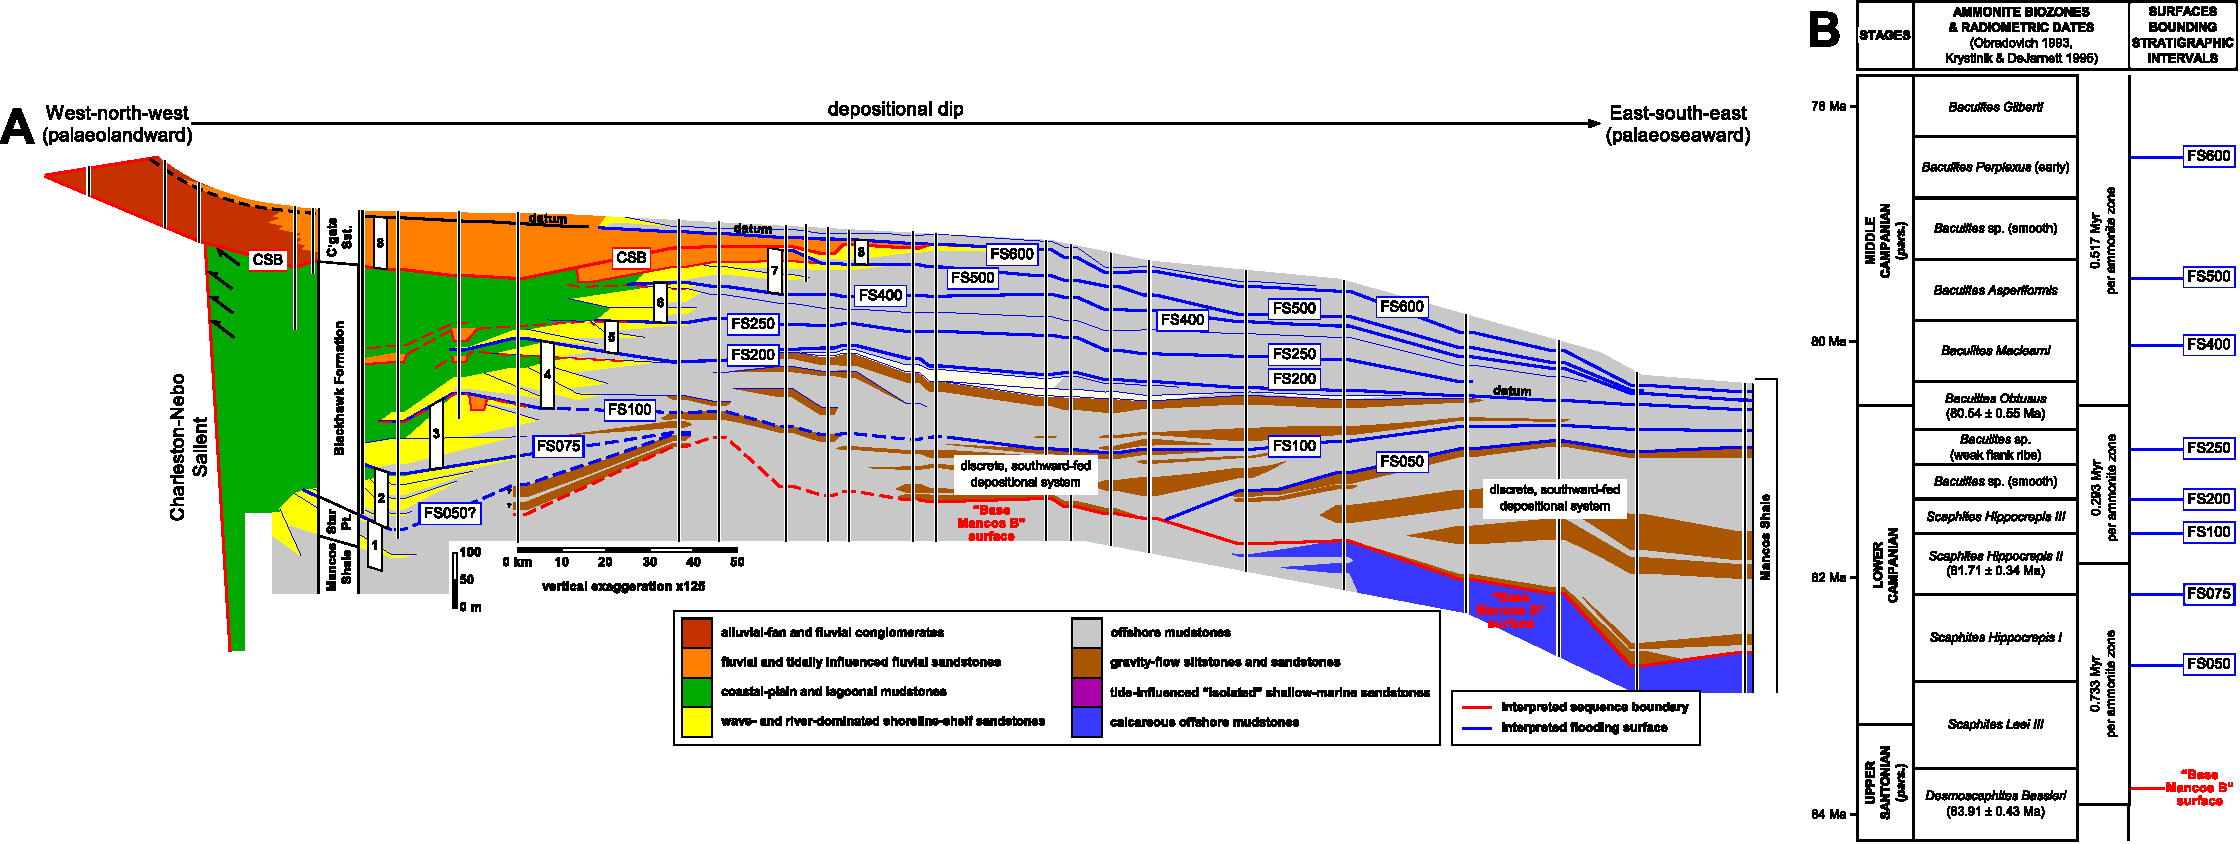
\includegraphics[width=\textwidth]{./figures/ch2-bookcliffs.pdf}
\caption{(a) Correlation panel illustrating stratigraphic architecture through the Book Cliffs outcrops and adjacent areas (after \citealp{horton-etal-2004,hampson-2010,hampson-etal-2014}; and references therein). Interpreted major flooding surfaces and erosional unconformities (sequence boundaries) are labelled. Deposits corresponding to time intervals 1-8 are indicated. Up system correlation of the lower part of the Castlegate Sandstone (time interval 8) is after \cite{robinson-1998} and \cite{mclaurin-2000}. A variety of stratigraphic surfaces are used as datum surfaces for different parts of the panel, and each surface is assigned the depositional dip of an eastward-dipping coastal plain or shelf profile where used as a datum. (b) Ammonite biostratigraphy, radiometric dates \citep{obradovich-1993}, and estimated ammonite biozone durations \citep{krystinik-1995} for the studied strata, showing the interpreted ages of major flooding.}
\label{fg:bookcliffs}
\end{figure}

The Book Cliffs of eastern Utah and western Colorado, USA, expose a record of a large palaeo-sediment-routing system. This is a classic site, where ancient clonglomeratic alluvial deposits transform into shoreline sandstones, marine deposits and shales (Figure \ref{fg:bookcliffs}). In collaboration with Philip Allen, Peter Burgess, and Gary Hampsen, we decided to explore if the migration of the gravel front, sand front, and shoreline within this sedimentary system could likewise be `inverted' for past forcing. The classic interpretation has been that cyclic progradation and retrogradation of the shoreline and sand front is due to cyclic sea level change (this is the birth place of sequence stratigraphy). The sediment transport equation (equation \ref{eq:transport}) was modified to include a transport law that was active when the surface was below sea level \citep{kaufman-etal-1991},
\begin{equation}
q_{s} = -\kappa_{sea}e^{-\kappa_{decay}\left(z_{sea}-z\right)}\frac{\partial z}{\partial x},
\end{equation}
where $\kappa_{sea}$ is the linear diffusion coefficient for subaqueous sediment transport. $\kappa_{decay}$ is the coefficient that parameterises the effect of water depth, $z_{sea}$, on subaqueous sediment transport. This heuristic model approximates the effect of tidal energy on moving sediment away from the shoreline. With this addition the effect of change in sea-level and surface run-off could be explored.

\begin{figure}
\centering
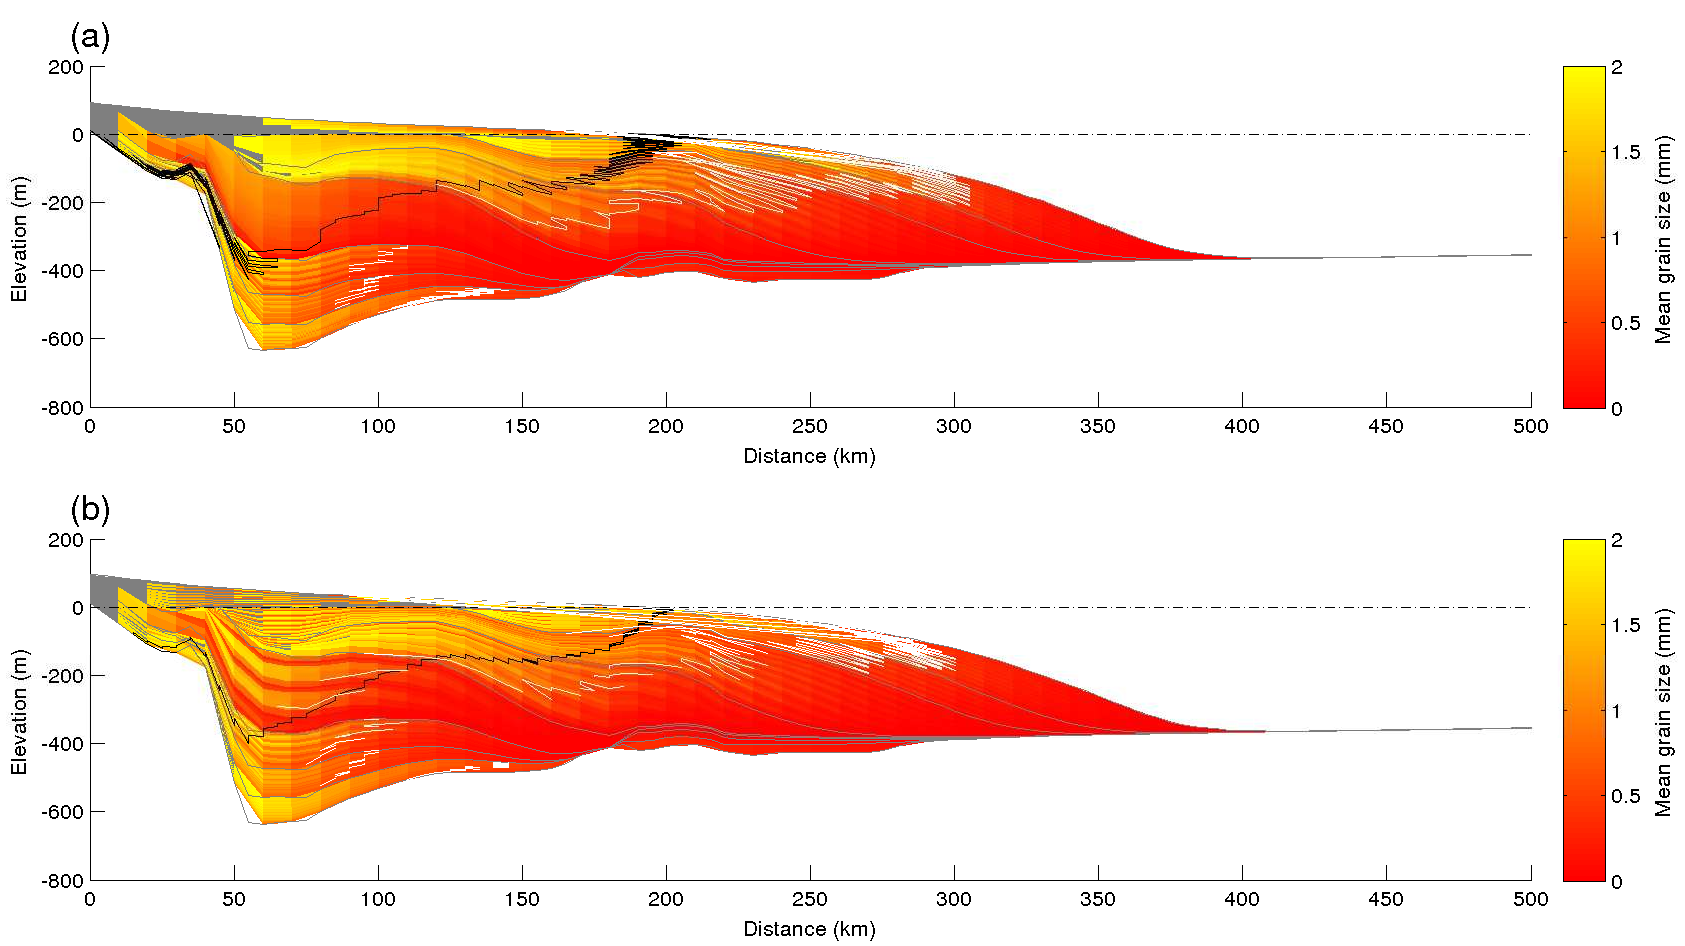
\includegraphics[width=10cm]{./figures/ch2-bookcliffs-model.pdf}
\caption{Synthetic strata for two models of the stratigraphic architecture in the Star Point -- Blackhawk -- lower Castlegate wedge, based on the Book Cliffs outcrops. (a) Predicted stratigraphic architecture assuming a 100\,kyr periodic oscillation in relative sea-level of amplitude $\pm 10\rm\,m$. (b) Predicted stratigraphic architecture assuming a 100\,kyr periodic oscillation in precipitation rate of amplitude $\pm 50$\,\%. Regions of gravel grains are blocked out in grey. The mean grain size of grains finer than 2\,mm in diameter is plotted. The shoreline position through time is marked as a solid black line, and the dashed black line marks sea level.}
\label{fg:bookcliffs-model}
\end{figure}

When the sediment transport model was applied to the Book Cliffs outcrop data the results showed that both high frequency (period of 100\,kyr) sea level change and change in surface run-off can impact the sand front and shoreline (Figure \ref{fg:bookcliffs-model}). However, change in terrestrial forcing also impacted the gravel front. If we assume that the observed depositional thickness of sediment is representative of the sediment flux into the basin, then the migration history of the gravel front would be a quantifiable measure to distinguish whether cyclical patterns of progradation and retrogradation were the result of cyclical change in precipitation rates or sea level (Figure \ref{fg:bookcliffs-model}). Data describing the architecture of proximal deposits in the Star Point -- Blackhawk -- lower Castlegate -- Mancos sediment-routing system are rare, however, on balance the evidence suggests limited movement of the gravel front. Therefore, a high-frequency cyclical change in relative sea level is the most probable of modelled mechanisms to account for the observed stratigraphic architecture. For a more detailed explanation see the full article in the Annex B.

This study, and the previous example from the Escanilla system, demonstrate the potential of applying physical models to test hypothesis (or interpretations) drawn from sedimentological observations. In both cases, the models gave insights into how the sedimentary system might respond to change, and how signals are transformed down system \citep{armitage-etal-ngeo-2011}. This style of model is currently being used to investigate late-Pleistocene to Holocene deposition in alluvial fans within Death Valley \citep[see][]{brooke-etal-2018}. Sam Brooke has advanced upon the transport model by adding infiltration, methods to account for storm variation, and a more physically based grain-size sorting. Early results would suggest that an increase in the frequency of storms will have just as a significant effect on the gravel front as an increase in mean run-off. 

\section{Predicting geological observations}

In Earth science the observations can become confused with interpretations. A tomographic image of the Earth's interior is not an observation, it is the result of an inversion and is therefore subject to various artefacts due to regularisation and the quality of the input data. Stratigraphic sections are images created by interpolating sparse observations of rock type and age, from which an image is created that gives a sense of the distribution of sedimentary deposits. A stratigraphic section, like a tomographic image, is not an observation. Yet, it is tempting to treat these models as observations.

The core of my research has been to try and use numerical models to predict observations. This has evolved from predicting crustal velocities, major element oxides, and rare Earth compositions in basaltic glass during my post PhD research \citep{armitage-etal-2010,armitage-etal-g3-2011}, to predicting grain size within sedimentary deposits in sedimentary basins \citep[e.g.][]{armitage-etal-ngeo-2011,armitage-etal-2015,armitage-etal-br-2018}, fan topography on Mars \citep{armitage-etal-grl-2011}, basin subsidence in various locations \citep[e.g.][]{armitage-2010,armitage-etal-jgr-2013,petersen-etal-2015}, upper mantle seismic tomography at various locations \citep[e.g.][]{goes-etal-2012,armitage-etal-2015}, and more. One of the biggest challenges has been breaking down the seismic inverse models and getting to the actual observation, the seismic waveform.

In a large collaborative effort with David Ferguson, Saskia Goes, James Hammond, Eric Calais, Kate Rychert and Nick Harmon, we tried to use both observations from igneous geochemistry and inverse models from seismic stations, to understand the structure of the upper mantle below Afar \citep{armitage-etal-epsl-2015}. Here I found that the forward geodynamic model could consistently predict the lava chemistry and seismic tomography from surface waves. However, it could not predict the seismic velocity structure required from the inversion of S-to-P receiver functions. From this failure I decided to build a research project where the seismic observation, the displacement recorded at the seismometer, would be predicted. This involved a new collaboration with Nobu Fuji, Alexandre Fournier, and our PhD student Thijs Franken. The result is a new scientific work-flow where the forward geodynamic model is transformed in to a seismic structure. This structure is used as an input for forward wave propagation, and the subsequent seismic arrival is compared with the arrival at the earth's surface (Figure \ref{fg:inversion}; \citealp{franken-etal-2020}). This is the first time that anyone has, to my knowledge, tried to compare a geodynamic model with a seismic observation, and I am convinced that this is the direction in which Earth science should go. The project does not end with the interpretation, this is simply the point of departure.

\begin{subappendices}

\section{A simplified model of decompression melting}

\begin{figure}
\centering
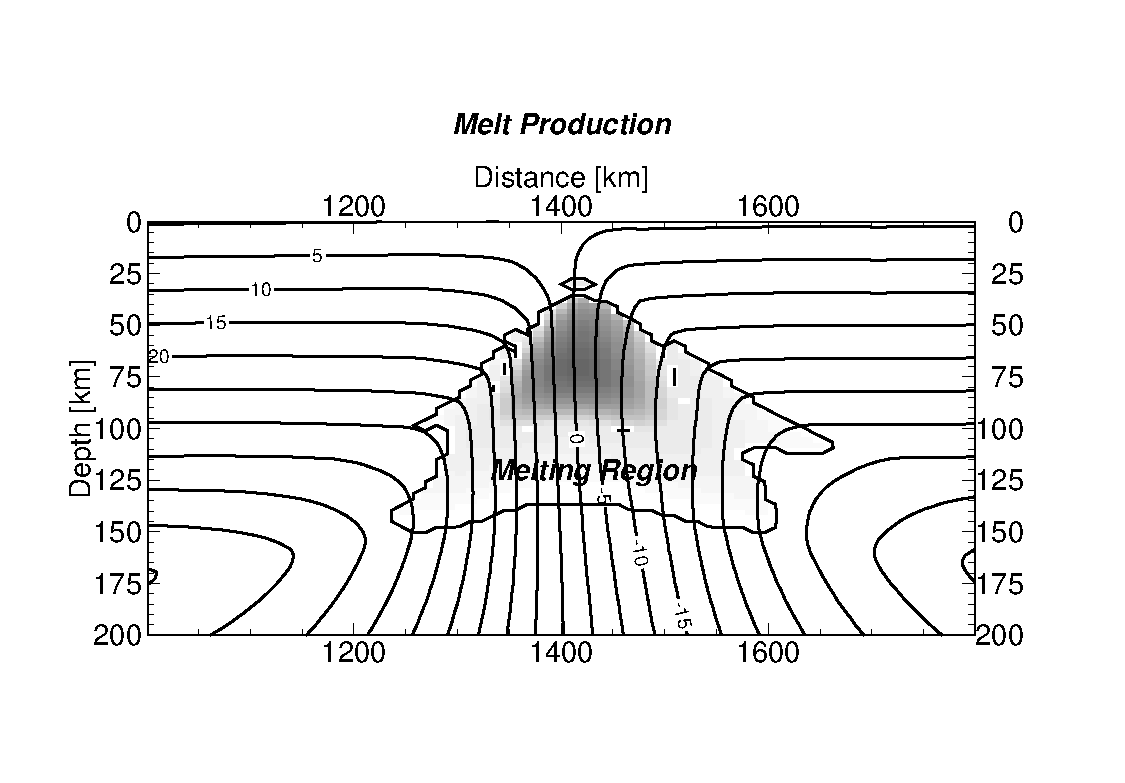
\includegraphics[width=8.6cm]{./figures/ch2-melt-region.pdf}
\caption{Diagram of the zone of partial melting with stream lines of mantle flow.}
\label{fg:melt-region}
\end{figure}

Decompression melting occurs when the mantle loses pressure due to vertical movement and the rock matrix crosses the solidus (Figure \ref{fg:melt-region}). To numerically model this process we need a set of continuum equations, which in this case are Stokes equations, the conservation of momentum and mass, and the conservation of energy. The conservation of momentum is,
\begin{equation}
\nabla \cdot \sigma + f = 0,
\end{equation}
where $\sigma$ is stress, the sum of the viscous stresses and pressure, and $f$ is the applied force, which in this case is due to gravity, $\Delta\rho g$. It is typical in geodynamics to then seperate out the viscous and pressure terms,
\begin{equation}
- \nabla \cdot \tau + \nabla p + \Delta\rho g \hat{\mathbf{z}} = 0,
\label{eq:momentum}
\end{equation}
where $\tau$ is the deviatoric stress, $p$ is pressure, $\Delta\rho$ is the density change due to thermal and chemical change (melting), $g$ is the acceleration due to gravity, and $\hat{\mathbf{z}}$ is a unit vector in the vertical direction.

The conservation of energy can be expressed as \citep[e.g.][]{ribe-1985},
\begin{equation}
\frac{\partial T}{\partial t} + \bar{\mathbf{v}} \cdot \nabla T - \kappa\nabla^{2} T + mL = 0,
\label{eq:energy}
\end{equation}
where $T$ is temperature, $\bar{\mathbf{v}}$ is the average velocity of the solid mantle and melt, $\kappa$ is the thermal diffusion coefficient, $m$ is the melt production rate, and $L$ is the latent heat of fusion. The latent heat is given by $L = T\Delta S/C_{p}$, where $\Delta S$ is the entropy change due to melting and $C_{p}$ is the heat capacity. The average velocity is given by \citep{scott-1992},
\begin{equation}
\bar{\mathbf{v}} = \left(1-\phi\right)\mathbf{v}_{s} + \phi \mathbf{v}_{l},
\label{eq:average-velocity}
\end{equation}
where $\phi$ is porosity, $\mathbf{v}_{s}$ is the solid mantle velocity, and $\mathbf{v}_{l}$ is the melt velocity. The conservation of mass is given by,
\begin{equation}
\frac{\partial \rho}{\partial t} + \nabla \cdot \left(\rho \bar{\mathbf{v}} \right) = 0.
\end{equation}
I take the simpligying assumption that density for the solid and liquid phase are the same, except for within the momentum balance, the \emph{Bousinesq approximation}. This means that the mass balance becomes,
\begin{equation}
\nabla \cdot \bar{\mathbf{v}} = 0
\label{eq:mass}
\end{equation}
In the case where there the melt phase is not explicitly modelled, the three equations can be solved various numerical methods such as finite difference \citep[e.g.][]{armitage-etal-g3-2018}, finite element \citep[e.g.][]{armitage-etal-2008}, or finite volume \citep[e.g.][]{civiero-etal-2019}.

If melt is to be included then the conservation of the liquid phase is written as,
\begin{equation}
\partial
\frac{\partial \phi}{\partial t} + \nabla \cdot \left( \phi \mathbf{v}_{l} \right) = m.
\label{eq:mass-melt}
\end{equation}
In this case to create a closed set of equations we need to relate the solid mantle velocity to the liquid melt velocity. If we assume that the melt percolates through a porous medium we can assume that the flows can be related by Darcy's law,
\begin{equation}
\phi\left( \mathbf{v}_{l}-\mathbf{v}_{s} \right) = \frac{k_{0}\phi^{n}}{\eta_{l}}\left( \Delta\rho_{m}g\hat{\mathbf{z}} + \nabla P \right),
\label{eq:darcy}
\end{equation}
where $k_{0}$ is the permeability coefficient (not well constrained), $n$ is the exponent on the assumed power relation between permeability and porosity, $\Delta\rho_{m}$ is the density difference between melt and the solid mantle, and $P$ is the pore pressure. I will simplify equation \ref{eq:darcy} by assuming that the compaction length scale is small, the `zero-compaction length approximation' \citep{ribe-1985}. This means that Darcy's law becomes,
\begin{equation}
\phi\left( \mathbf{v}_{l}-\mathbf{v}_{s} \right) = \frac{k_{0}\phi^{n}}{\eta_{l}}\Delta\rho_{m}g\hat{\mathbf{z}},
\end{equation}
and by substituting for the average velocity (equation \ref{eq:average-velocity}) we get and considering the veritcal flow only,
\begin{equation}
v_{l}-\bar{v} = \frac{k_{0}\phi^{n-1}}{\eta_{l}}\Delta\rho_{m}g.
\end{equation}
This allows the substitution for $v_{l}$ within equation \ref{eq:mass-melt}. However there remains one fundamental unknown, and that is the relationship between permeability and porosity. The value of $n$ in equation \ref{eq:darcy} is estimated to between 2 and 3. The most recent laboratory experiments would suggest that for mantle rock $n = 2.6\pm0.2$ \citep{miller-etal-2014}. Mathematically it is more expedient to assume that $n$ is an integer, therefore it has been assumed to be either 2 \citep[e.g.][]{scott-1989,goes-etal-2012} or 3 \citep[e.g.][]{hewitt-2010,armitage-etal-grl-2019}. Assuming $n=3$ the conservation of melt can be written as,
\begin{equation}
\frac{\partial \phi}{\partial t} + \bar{v}\frac{\partial \phi}{\partial z} + \frac{3k_{0}\Delta\rho_{m}g}{\eta_{l}}\phi^{2}\left( 1-\frac{4}{3}\phi \right)\frac{\partial \phi}{\partial z} = m.
\end{equation}
This non-linear 1D partial differential can be solved numerically using various iterative techniques \citep[e.g.][]{armitage-etal-grl-2019,franken-etal-2020}.

\begin{figure}
\centering
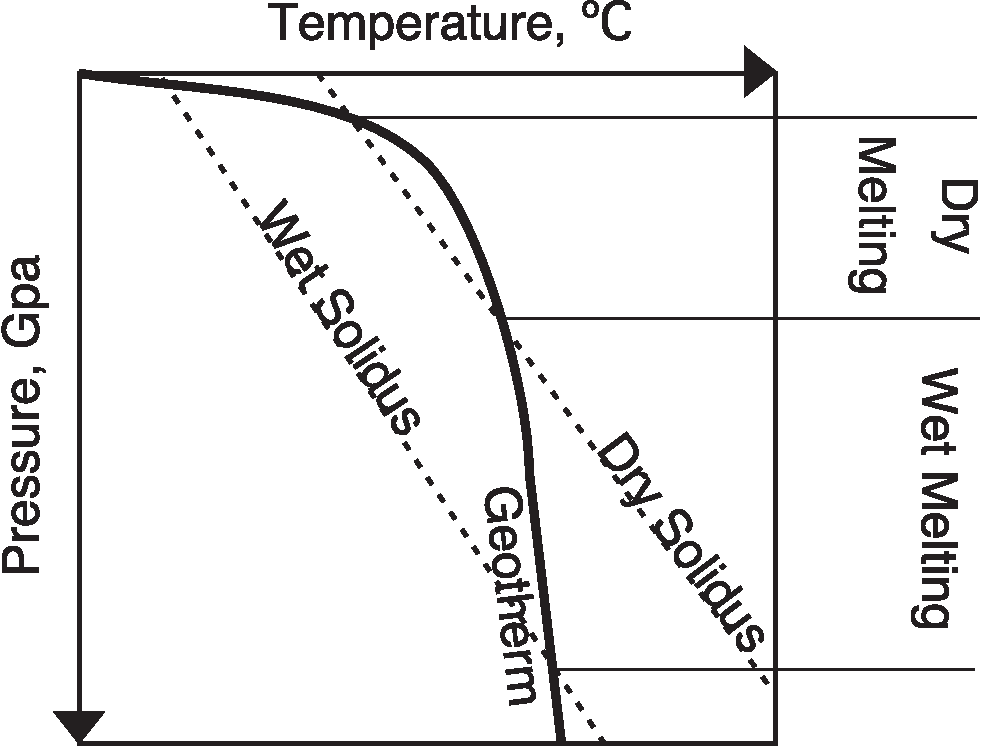
\includegraphics[width=8.6cm]{./figures/ch2-solidi-geotherm.pdf}
\caption{Diagram of the mantle geotherm crossing the wet and dry solidus.}
\label{fg:solidus}
\end{figure}

The conservation of energy and mass are coupled by the melt production rate, which is calculated from the temperature difference above the solidus. This solidus is a function of volatile content, depletion, temperature, and pressure (Figure \ref{fg:solidus}). In the energy balance I ignore the loss of heat due to decompression, but the adiabatic gradient needs to be accounted for within the thermodynamic balance for the melting equations. Assuming the mantle is dehydrated, no volatiles, it is calculated as,
\begin{equation}
T_{Sdry} = T_{S0} + \frac{\partial T_{S}}{\partial F}\vert_{p}F + \left(\frac{\partial T_{S}}{\partial p}\vert_{F} + \frac{\alpha T_{0}}{\rho C_{p}}\right)p,
\label{eq:dry-solidus}
\end{equation}
where $\partial T_{S}/\partial F\vert_{p}$ is the solidus depletion gradient, $F$ is depletion, $\partial T_{S}/\partial P\vert_{F}$ is the solidus pressure gradient, $\alpha$ is the coefficient of thermal expansion, $T_{0}$ is the mantle potential temperature, $C_{p}$ is the heat capacity, and $p$ is pressure. The solidus is assumed to deepen in the presence of water,
\begin{equation}
T_{Swet} = T_{Sdry} + K\left(D_{H_{2}O}C_{H_{2}O}\right)^{\gamma},
\label{eq:wet-solidus}
\end{equation}
where the coefficients $K$ and $\gamma$ are from the parametrisation of \cite{katz-etal-2003}, $D_{H_{2}O}$ is the partition coefficient for water, and $C_{H_{2}O}$ is the concentration of water within the solid mantle. Therefore the melt productivity is given by,
\begin{equation}
m = \frac{\Delta T}{L + \frac{\partial T_{S}}{\partial F}\vert_{P} + \frac{\partial T_{S}}{\partial F}\vert_{H_{2}O}},
\label{eq:melt-productivity}
\end{equation}
where $\Delta T = T-T_{S}$ is the temperature difference between the mantle and the solidus, and $\partial T_{S}/\partial F\vert_{H_{2}O}$ is the solidus depletion gradient during the melting of a hydrated mantle. This is calculated using the chain rule,
\begin{equation}
\frac{\partial T_{S}}{\partial F}\vert_{H_{2}O} = \frac{\partial T_{S}}{\partial C_{H_{2}O}} \frac{\partial C_{H_{2}O}}{\partial F}.
\end{equation}
The change in water composition as a function of depletion is calculated  assuming a mass balance between the partitioning of water between the solid and melt phase,
\begin{equation}
\frac{\partial C_{H_{2}O}}{\partial F} = -C_{H_{2}O} \frac{1}{D_{H_{2}O}}\left(1-F\right)^{\frac{1}{D_{H_{2}O}}-2}
\end{equation}
and the gradient in solidus with water composition is from equation \ref{eq:wet-solidus},
\begin{equation}
\frac{\partial T_{S}}{\partial C_{H_{2}O}} = \gamma K\left(D_{H_{2}O}C_{H_{2}O}\right)^{\gamma-1}
\end{equation}

To track the composition of the melt I assume disequilibrium melting, where the conservation of the solid composition, $C_{s}$, is given as \citep{spiegelman-1996},
\begin{equation}
\frac{\partial C_{s}}{\partial t} + v_{s}\frac{\partial C_{s}}{\partial z} = \left(\frac{1}{D} - 1\right) \frac{C_{s}m}{1-\phi},
\label{eq:solid-composition}
\end{equation}
and the melt composition, $C_{l}$, can be written as follows \citep{spiegelman-1996},
\begin{equation}
\frac{\partial C_{l}}{\partial t} + v_{l}\frac{\partial C_{f}}{\partial z} = \left(\frac{C_{S}}{D} - C_{l}\right)\frac{m}{\phi}.
\label{eq:melt-composition}
\end{equation}
The melt composition is calculated from the solid composition and knowledge of the partition coefficient $D$. The partition coefficient is a function of the mineral phase stability \citep{mckenzie-1991},
\begin{equation}
D = f_{ol}\mathcal{D}_{ol\rightarrow melt} + f_{opx}\mathcal{D}_{opx\rightarrow melt} + f_{cpx}\mathcal{D}_{cpx\rightarrow melt} + f_{X}\mathcal{D}_{X\rightarrow melt}
\label{eq:onions}
\end{equation}
where $f$ is the proportion of each mineral within plagiolcase, spinel, and garnet peridotite, $D_{ol}$, etc, are the partition coefficients for for each phase into melt, and $X$ represents plagioclase, spinel and garnet, respectively \citep[e.g.][]{armitage-etal-g3-2011,armitage-etal-g3-2018}.

The above set of equations, which are arguably an over simplification, allow for the tracking of key parameters that control the surface seismic and chemical observations. Melt depletion, porosity, temperature and depth can be converted into major, trace and rare Earth element compositions for comparison with observations from erupted lava and the P-wave velocity of the crust (Figure \ref{fg:4models}; \citealp{armitage-etal-2008,armitage-etal-2009,armitage-etal-2010,armitage-etal-g3-2011,armitage-etal-epsl-2015,armitage-etal-g3-2018,armitage-etal-grl-2019}). Temperature, pressure, composition and porosity can be converted to density, bulk, and shear modulus to then be converted into synthetic tomographic images (Figure \ref{fg:mantleVs}; \citealp{goes-etal-2012,armitage-etal-epsl-2015,armitage-etal-g3-2018,armitage-etal-grl-2019}).

\section{A simplified model of surface processes}\label{subsec:a-simplified-model-of-surface-processes}

\begin{figure}
\centering
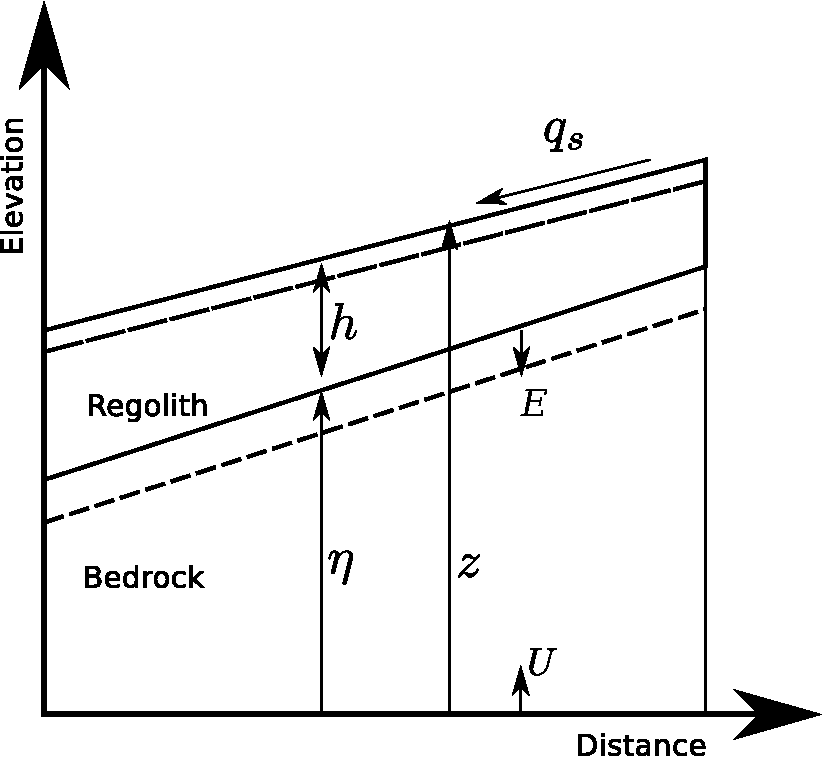
\includegraphics[width=8.6cm]{./figures/ch2-erosion-diagram.pdf}
\caption{Diagram showing the conservation of mass within a 2-D domain, where mass enters the system through uplift, $U$, and exists as sediment transported, $\mathbf{q}_{s}$ out of the domain. $E$ is the rate of production of regolith, $h$ is the thickness of regolith, $\eta$ is the bedrock elevation and $z$ is the total elevation.}
\label{fg:1dmodel}
\end{figure}

Following \cite{dietrich-etal-2003} I define a landscape of elevation $z$ composed of bedrock, thickness $\eta$, and a surface layer of sediment with thickness $h$ (Figure \ref{fg:1dmodel}). This landscape is forced externally through uplift rate $U$. The bedrock is transferred into sediment through erosion at a rate $E$ and the sediment is transported across the system with a flux $\mathbf{q}_{s}$. Assuming that the density of sediment and bedrock are equal, then the change in bedrock thickness is,
\begin{equation}
\frac{\partial\eta}{\partial t} = U - E,
\label{eq:bedrock}
\end{equation}
and the rate of change in sediment thickness is,
\begin{equation}
\frac{\partial h}{\partial t} = E - \nabla \cdot \mathbf{q}_{s}.
\label{eq:sediment}
\end{equation}
It then follows that the rate of change in landscape elevation is,
\begin{equation}
\frac{\partial z}{\partial t} = \frac{\partial\eta}{\partial t} + \frac{\partial h}{\partial t}.
\label{eq:elevation}
\end{equation}

To solve the mass balance I will make a strong assumption: there is always a supply of transportable sediment. Then I can follow through with the summation in equation \ref{eq:elevation} giving,
\begin{equation}
\frac{\partial z}{\partial t} = U - \nabla \cdot  \mathbf{q}_{s}.
\end{equation}
This may be appropriate when modelling the transport of sediment along the river bed and when considering the formation of alluvial fans \citep[e.g.][]{paola-etal-1992,whipple-2002,guerit-etal-2014}. In the absence of surface water we can assume that sediment flux is simply a function of local slope $\mathbf{q}_{s} = -\kappa\nabla z$. In the presence of flowing water then the sediment flux is a function of the flowing water and local slope $\mathbf{q}_{s} = -c\mathbf{q}_{w}^{\delta}\left(\nabla z\right)^{\gamma}$ where $c$ is the transport coefficient (units (m$^{2}$\,yr$^{-1}$)$^{1-\delta}$), $\mathbf{q}_{w}$ is the water flux per unit width, and the exponents $\delta > 1$ and $\gamma \geq 1$ are dependent on how sediment grains are transported along the bed \citep{smith-1972,paola-etal-1992}. Furthermore, $\delta > 1$ is required to create concentrated flow \citep{smith-1972}. The change in landscape elevation is then given by,
\begin{equation}
\frac{\partial z}{\partial t} = U + \nabla \cdot \left(\kappa\nabla z +c\mathbf{q}_{w}^{\delta}\left(\nabla z\right)^{\gamma}\right).
\end{equation}
which can be written as,
\begin{equation}
\frac{\partial z}{\partial t} = U + \nabla \cdot \left(\left[\kappa +c\mathbf{q}_{w}^{\delta}\left(\nabla z\right)^{\gamma-1}\right]\nabla z\right).
\label{eq:transport}
\end{equation}
Equation \ref{eq:transport} is non-linear in the case that $\gamma \neq 1$. In deriving this equation of elevation change due to sediment transport we have simply summed the two terms for sediment flux, the linear and potentially non-linear slope dependent terms. This summation has been done as it is the simplest way to generate landscape profiles that have the desired convex and concave elements observed in natural landscapes \citep{smith-1972}.

To solve this equation in one dimension I assume that the water flux is a function of the precipitation transported down the river network. The water collected is taken from the upstream drainage area, $a$, which is related to the main stream length, $l$, by $l \propto a^{h}$ where $h$ is the exponent taken from the empirical Hack's law \citep{hack-1957}. The main stream length is related to the longitudinal length of the catchment by, $l \propto x^{d}$ where $1 \leq d \leq 1.1$ \citep{tarboton-etal-1990,maritan-etal-1996}. Therefore, we can write that $x \propto a^{h/d}$, and the water flux is the precipitation rate, $\alpha$ units (m\,yr$^{-1}$), multiplied by the length of the drainage system,
\begin{equation}
q_{w} = k_{w}\alpha x^{p}
\label{eq:waterflux}
\end{equation}
where $k_{w}$ is the width coefficient (units m$^{1-p}$), and $p = d/h$. Furthermore it is observed that river catchments are typically longer than they are wide, and so $p<2$ \citep{dodds-2000a}. Therefore given that $0.5 < h < 0.7$ \citep[e.g.][]{rigon-etal-1996} then $1.4 < p < 2$, and the transport model (equation \ref{eq:transport}) becomes,
\begin{equation}
\frac{\partial z}{\partial t} = U + \frac{\partial}{\partial x} \left(\left[\kappa +ck_{w}\alpha^{\delta}x^{p\delta}\left(\frac{\partial z}{\partial x}\right)^{\gamma-1}\right]\frac{\partial z}{\partial x}\right).
\label{eq:1dtransport}
\end{equation}

\begin{figure}
\centering
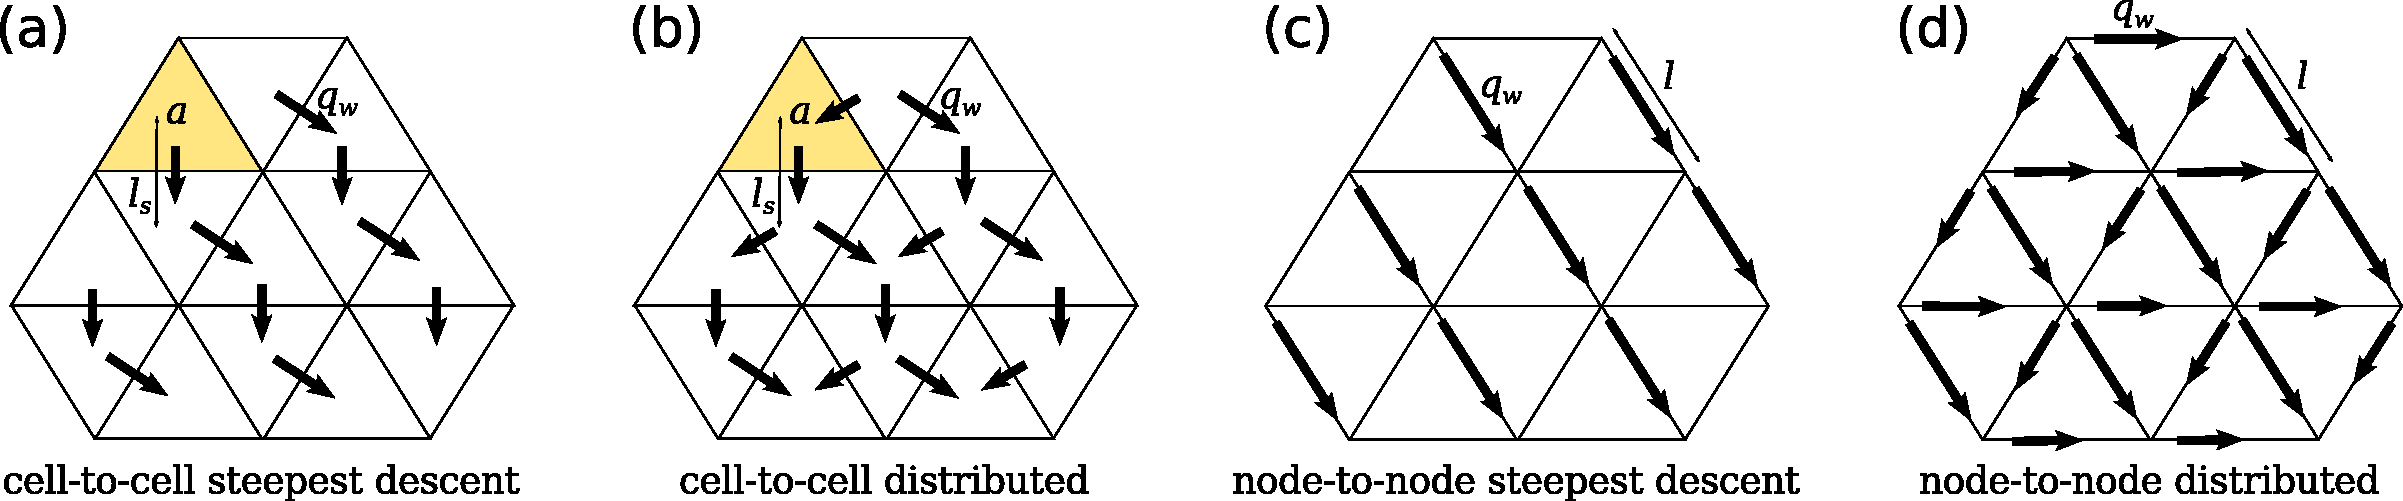
\includegraphics[width=\textwidth]{./figures/ch2-routing.pdf}
\caption{Diagram of flow routing from cell-to-cell and node-to-node for either a single flow direction (SFD) and a multiple flow direction (MFD) algorithm weighted by the relative gradient.}
\label{fg:routing}
\end{figure}

To solve equation \ref{eq:transport} over a 2-D domain requires an algorithm to route surface flow down the landscape. Water can be routed from cell-to-cell, where precipitation is collected over the area of each cell, sent downwards, and accumulates. In this cell-to-cell configuration the water flux has units of length squared per unit time and is given by:
\begin{equation}
q_{w}\mathrm{[cell]} = \frac{\alpha a}{l_{s}},
\label{eq:cell}
\end{equation}
where $\alpha$ is precipitation rate, $a$ is the cell area, and $l{s}$ is the length from cell centre to cell centre down the steepest slope (Figure \ref{fg:routing}a and b). This gives a water discharge per unit length, which has the advantage of not having to explicitly state the sub-grid width of the flow \citep{simpson-2003}. However, implicitly this implies that the flow is over the width of a cell. An alternative is to route water from node to node along cell edges and for it to accumulate. I assume that along the length of each cell edge water can be added to the flow line, assuming that the input is linearly related to the length of the flow line,
\begin{equation}
q_{w}\mathrm{[node]} = \alpha l,
\label{eq:node}
\end{equation}
where $l$ is the length of the edge that joins the up-slope node to the down-slope node (Figure \ref{fg:routing}c and d). This means that the cell area is ignored and instead water enters the flow path uniformly along its length and accumulates down slope.

Equation \ref{eq:node} makes the assumption that water accumulates as a function of length. Water flux is observed to related to catchment area, $Q_{w} \propto A^{0.8}$ \citep{syvitski-2007}. The catchment length, $l$ is then related to area by, $l\propto A^{1/p}$, where $1.4<p<2.0$ \citep{armitage-etal-esurf-2018}. At the lower end of the range this gives $Q_{w} \propto l^{1.12}$, suggesting that accumulating water as a linear function of flow length is a reasonable simplification. A knock on effect of this assumption is that the magnitude of the water flux predicted for the node-to-node routing is less than the cell-to-cell, as in the latter water is accumulated over cell areas, which is naturally larger than the cells edges.

Both equations \ref{eq:cell} and \ref{eq:node} do not attempt to capture the interaction between water flux and river width, rather these are two methods to approximate run-off within a coarse numerical grid. For both the cell-to-cell and node-to-node methods the flow can then be routed down a single flow direction (SFD) or routed down multiple flow directions (MFD) weighted by the relative gradient, as in for example \cite{schoorl-etal-2000}. The choice of flow routing has a large effect on the numerical solution. I showed that SFD creates a numerical solution that is highly resolution dependent \citep{armitage-2019}. It is only by using the MFD routing that model solutions are not resolution dependent (see code fLEM\footnote{fLEM: Fenics based Landscape Evolution Model, see \url{https://github.com/johnjarmitage/flem}}, Figure \ref{fg:MFD}, \citealp{armitage-2019}).

\begin{figure}
\centering
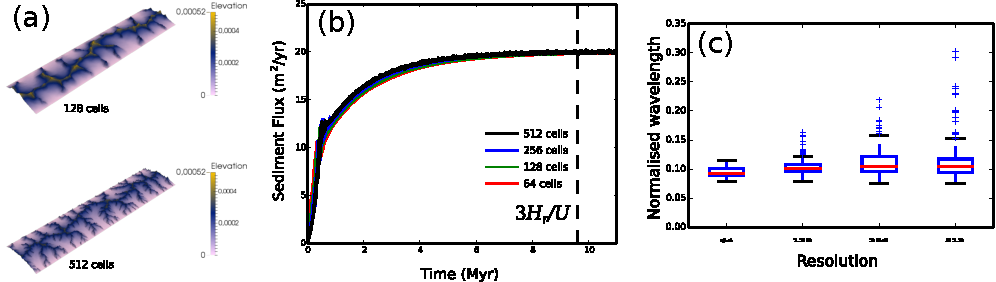
\includegraphics[width=\textwidth]{./figures/ch2-MFD.pdf}
\caption{A landscape evolution model fLEM \citep{armitage-2019}. (a) Dimensionless elevation from the node-to-node flow routing landscape evolution model with different flow routing algorithms at different numerical resolutions after a dimensionless run time of $1.563\times10^{-6}$ (5\,Myr), with an aspect ratio of $4\times1$. (b) Dimensional sediment flux that exits the model domain. (c) Box whisker plots of the dimensionless valley-to-valley wavelength for each model for different resolutions, where the number of cells along the y-axis is shown.}
\label{fg:MFD}
\end{figure}

The sediment flux generated by erosion within the model and the accommodation space generated by subsidence can be used to generate grain size profiles of the stratigraphic layers. The 1D down-system grain-size distribution is modified down-system by selective deposition following the theoretical model and observations of \cite{fedele-2007} and \cite{duller-etal-2010}. I assume perfect sorting, where only gravel is deposited until it is exhausted, followed by only sand and finally by fine-grained material (silt and clay grade; \citealp{paola-etal-1992}). Gravel undergoes fining according to an exponential function of Sternberg type \citep{fedele-2007,duller-etal-2010},
\begin{equation}
D(\tilde{x}) = D_{g0} + \phi_{0}\frac{1}{C_{v}}\left( e^{-C_{g}\tilde{y}}-1 \right).
\label{eq:fedele}
\end{equation}
The fining of the sand and smaller grain sizes is given by \cite{sternberg-1875},
\begin{equation}
D(\tilde{x}) = D_{si}e^{-C_{s}\tilde{y}}.
\label{eq:sternberg}
\end{equation}
In equations \ref{eq:fedele} and \ref{eq:sternberg} $\tilde{x}$ is the dimensionless down-system length, $D_{g0} = log_{10}\left(D_{50}\right)$ is the median of the gravel input taken from the 50th percentile from Wolman pebble-count data, $\phi_{0} = log_{10}\left( D_{84}/D_{50} \right)$ is the input variance of the gravel assuming that the distribution is log-normal, $D_{si} = log_{10}\left( 2\,{\rm mm} \right)$ is the initial grain-size for sand and finer material in the sediment input, and $\tilde{y}$ is the spatial transformation of the down-system distance given by \citep{paola-1995},
\begin{equation}
\frac{d\tilde{y}}{d\tilde{x}} = \frac{r}{q_{s}}
\end{equation}
where $r$ is the down-system distribution of deposition and $q_{s}$ is the down-system distribution of sediment discharge.

\end{subappendices}

\chapter{Perspectives}

My research outlook over the coming decade is going to shift away from studying the Earth's deep interior and move towards the surface. In the next century run-off, which drives fluvial erosion, will likely change significantly due to the effects of global warming on the Earth system. To quote the IPCC's Fifth Assessment Report \cite{IPCC-policy-2014}:

\begin{displayquote}
In many regions, changing precipitation or melting snow and ice are altering hydrological systems, affecting water resources in terms of quantity and quality (medium confidence). Glaciers continue to shrink almost worldwide due to climate change (high confidence), affecting run-off and water resources downstream (medium confidence). Climate change is causing permafrost warming and thawing in high-latitude regions and in high-elevation regions (high confidence).
\end{displayquote}

The impact of such change on sediment storage and transport is uncertain. We can look to the past for evidence of how fluvial systems have responded, but at a time scale of hundreds of years it can become difficult to distinguish the importance of events such as individual storms. Furthermore, as I will expand upon below, there is a broad range of different numerical models developed to study landscape change on different time and spatial scales. One key process is being overlooked: groundwater. Beyond simple empirical laws for 1D infiltration, no numerical models to my knowledge include the impact of groundwater flow on the evolution of fluvial erosion and deposition. Yet rivers recharge by not only by surface run-off but from the ground \citep[e.g.][]{condon-etal-2020}, and river networks most likely grow as a network within the partially saturated ground \citep[e.g.][]{fan-etal-2019}. The challenge is to translate this concept into a testable model that can be applied to fluvial systems.

\section{Short-Term: Non-steady surface water flow}

Landscape evolution modelling on geological time-scales ($>10^{4}$\,yr) has been dominated by one single equation: the stream power law \citep[see][]{howard-1983,howard-1994}. If I return to the simple diagram of surface processes (Figure \ref{fg:1dmodel}), the stream power law makes one very sweeping assumption: the rate of change in sediment thickness within the landscape is zero, which is to say all sediment created is transported out of the model domain. Furthermore, assuming surface flow is the primary driver of landscape erosion and that positive $x$ is in the downstream direction then erosion, $E$, as a function of the power of the flow to detach particles of rock per unit width can be written as,
\begin{equation}
E = -k_{b}\rho_{w}g\mathbf{q}_{w}^{m} \cdot \left(\nabla z\right)^{n},
\label{eq:streampower-inv}
\end{equation}
where $k_{b}$ is a dimensional constant that parametrises bedrock erodability \citep{howard-1983}, $\rho_{w}$ is water density, $g$ is gravity, $q_{w}$ is water flux per unit width, $m$ and $n$ are constants. The exponent $m \sim 0.5$, as it is a function of how the stream flow width is proportional to the water flux \citep[e.g.][]{lacey-1930}. The exponent $n>0$ acts upon the slope. In two dimensions the change in elevation is then given by,
\begin{equation}
\frac{\partial z}{\partial t} = U + k\mathbf{q}_{w}^{m} \cdot \left(\nabla z\right)^{n},
\label{eq:streampower}
\end{equation}
where the constant $k$ lumps together the other constants, and if $n\neq1$ equation \ref{eq:streampower} becomes non-linear. But in any landscape, the assumption of instantaneous sediment transport does not hold. The above model does not work. This raises a question: {\bf what are the key processes within landscape evolution?}

The question of what processes dominates in landscape evolution becomes more important as the time scale of interested becomes shorter. This has lead tot he development of process based landscape evolution models (LEMs) for various applications \citep[see for example][]{temme-etal-2017}. I will briefly describe two that have been used to study landscape change over different time-scales:
\begin{itemize}
\item[1] {\bf LAPSUS}
This is a process based model, where sediment is eroded or deposited down slope based on the transport capacity of the fluvial system \citep{schoorl-etal-2000}. It also includes processes such as soil formation and solid creep. It is a highly simplistic model with eight free parameters which can vary in space and time.
\item[2] {\bf CAESAR-Lisflood}
This is a process based model but of increased complexity compared to LAPSUS. It is based on a cellular automaton approach, but the laws acting on each cell are many and complex. Overland flow is modelled using the Lisflood model of \cite{bates-etal-2010}, and a simple infiltration is included using TOPMODEL \citep{beven-1979}. Subsequently sediment is transported down slope given the shear velocity of the flow is sufficiently high \citep{coulthard-etal-2013,vandeweil-etal-2007}. Other processes are included such as soil creation, lateral erosion, vegetation cover, etc., giving a total of 49 free parameters \citep{skinner-etal-2018}.
\end{itemize}
Given the number of processes typically modelled in LEMs it is difficult to assess which are significant and those to which there is no sensitivity. Recently sensitivity analysis has been carried for CAESAR-Lisflood out using a part of the full parameter space \citep{skinner-etal-2018}. The result of this sensitivity analysis is that the greatest sensitivity was to the sediment transport law, which is a function of the flow of water. This is a first order variable within the model, and it suggests second order aspects such as the degree of vegetation, soil creation are of lower importance.

\begin{figure}
\begin{minipage}{\textwidth}
\begin{minipage}{.5\textwidth}
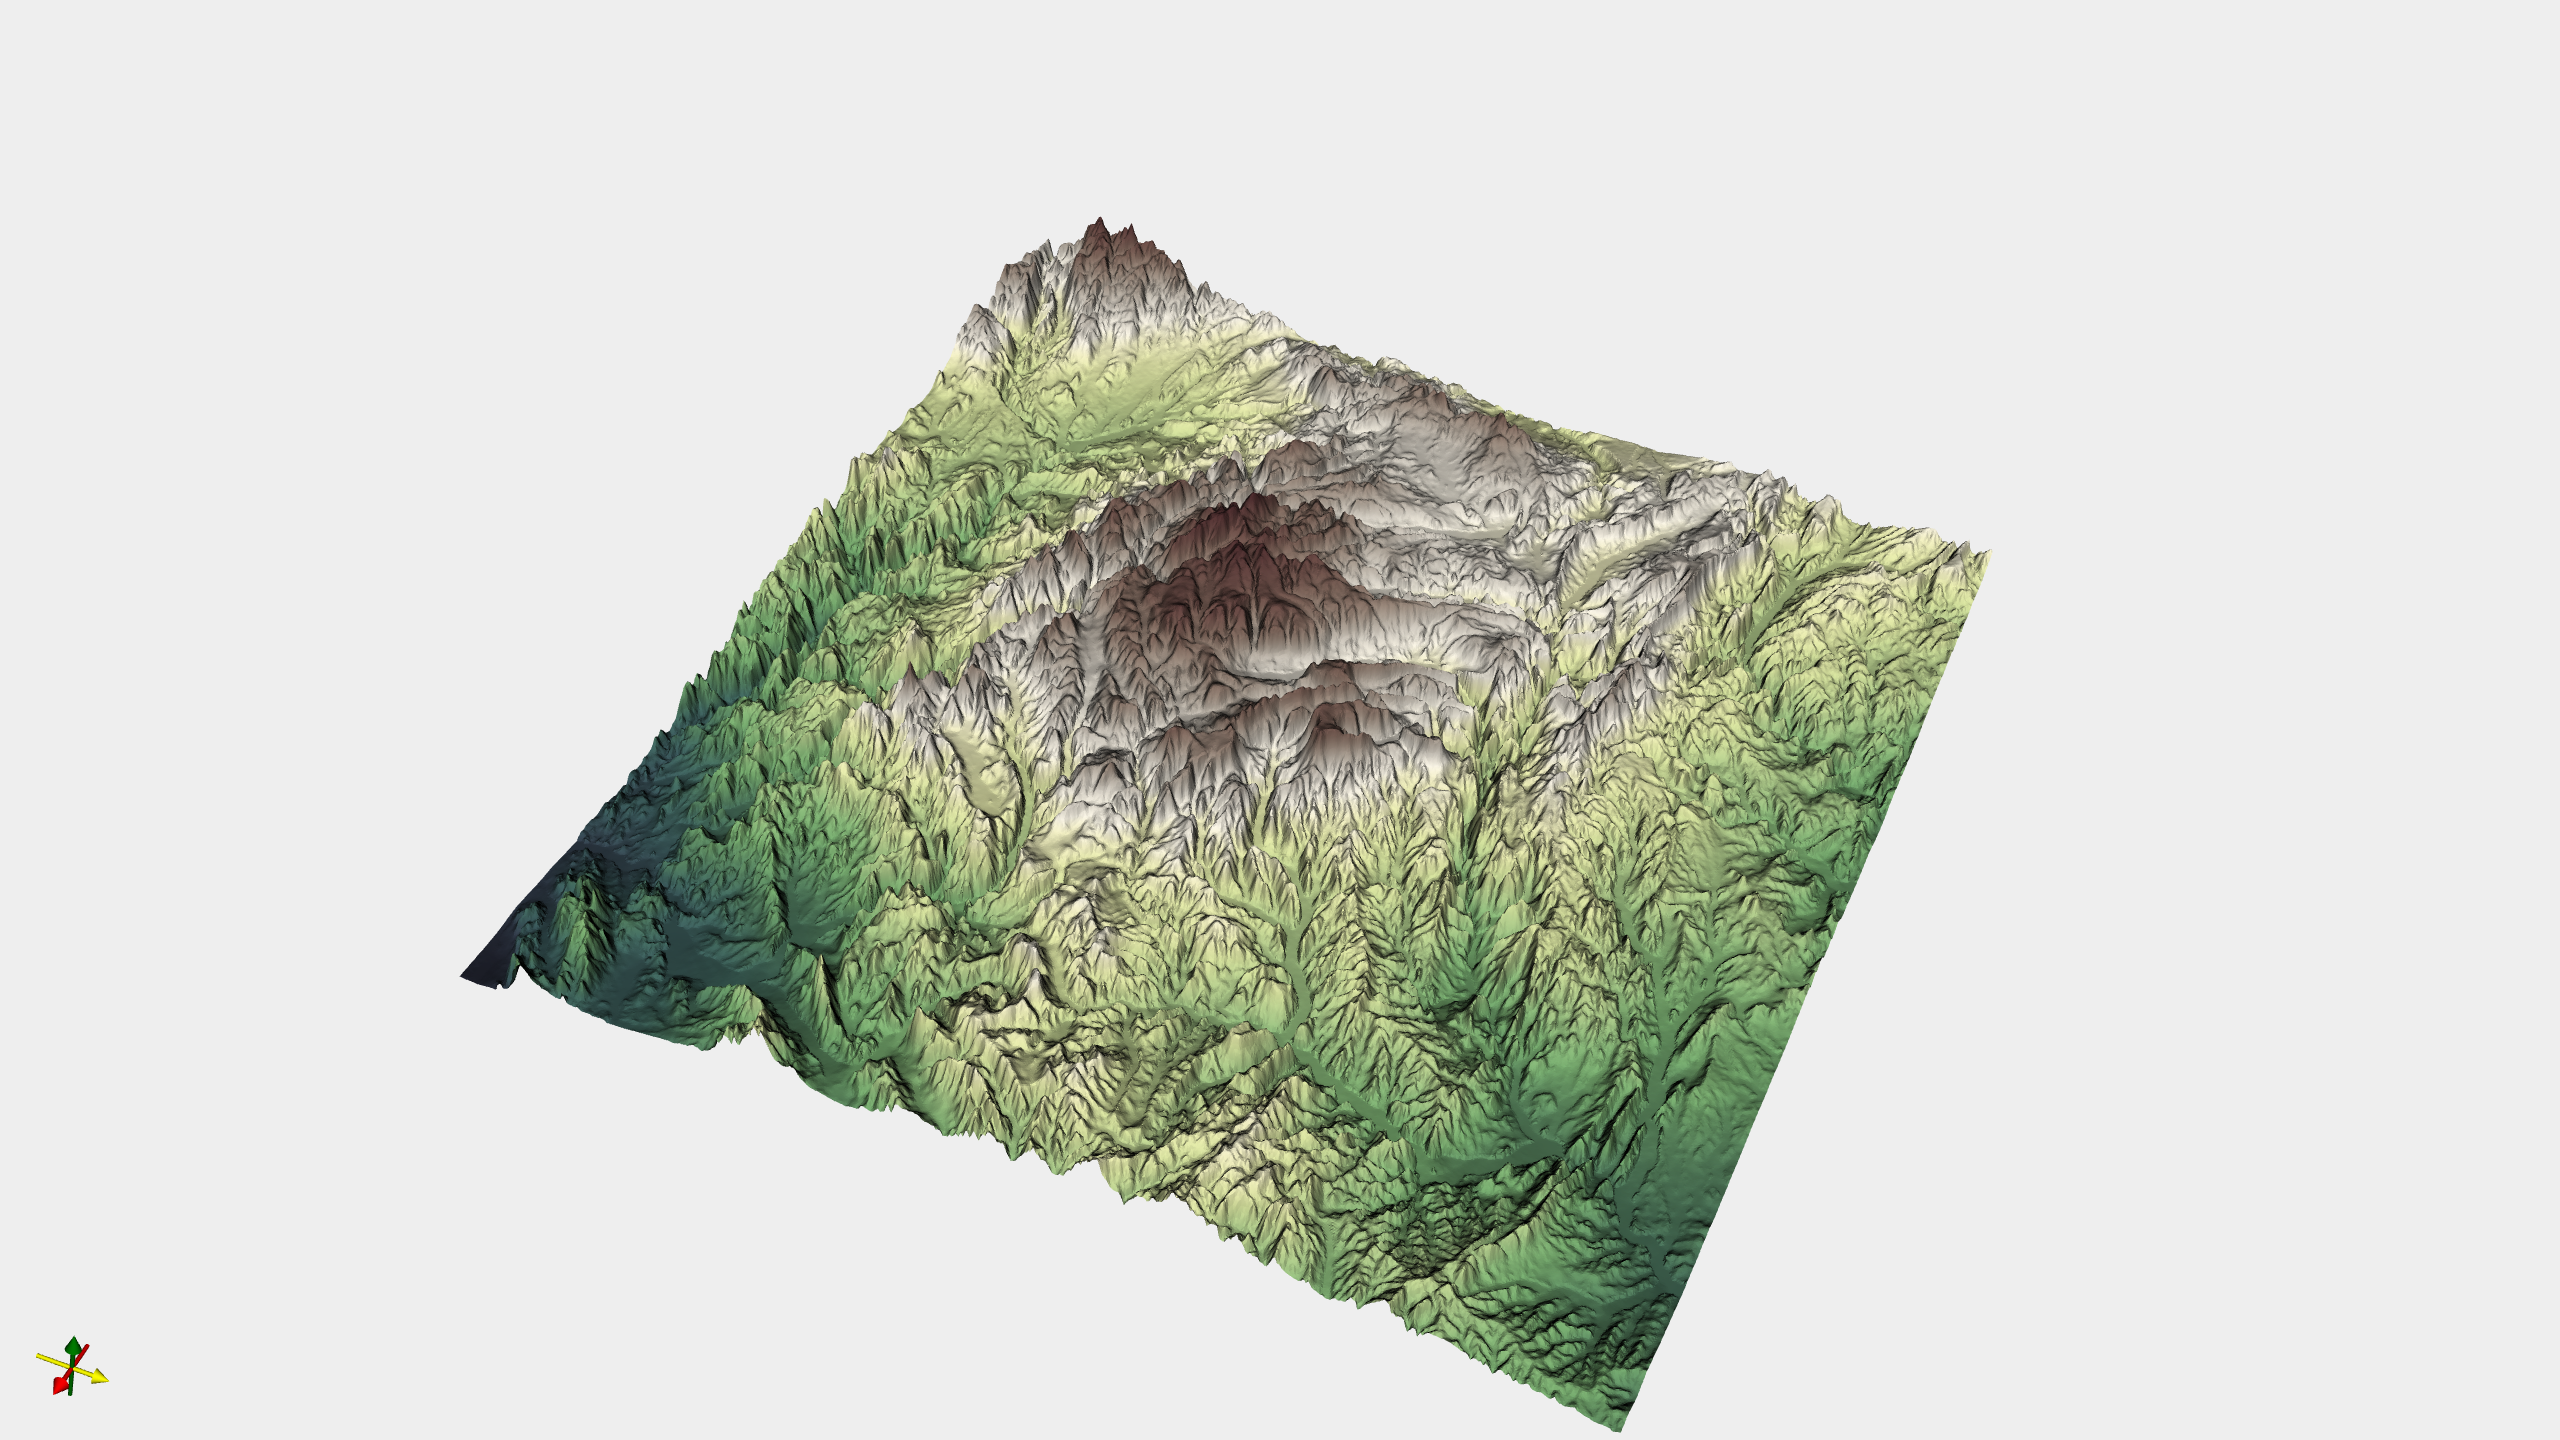
\includegraphics[width=.98\textwidth]{./figures/ch3-bergantes-elevation.png}
\end{minipage}
\begin{minipage}{.5\textwidth}
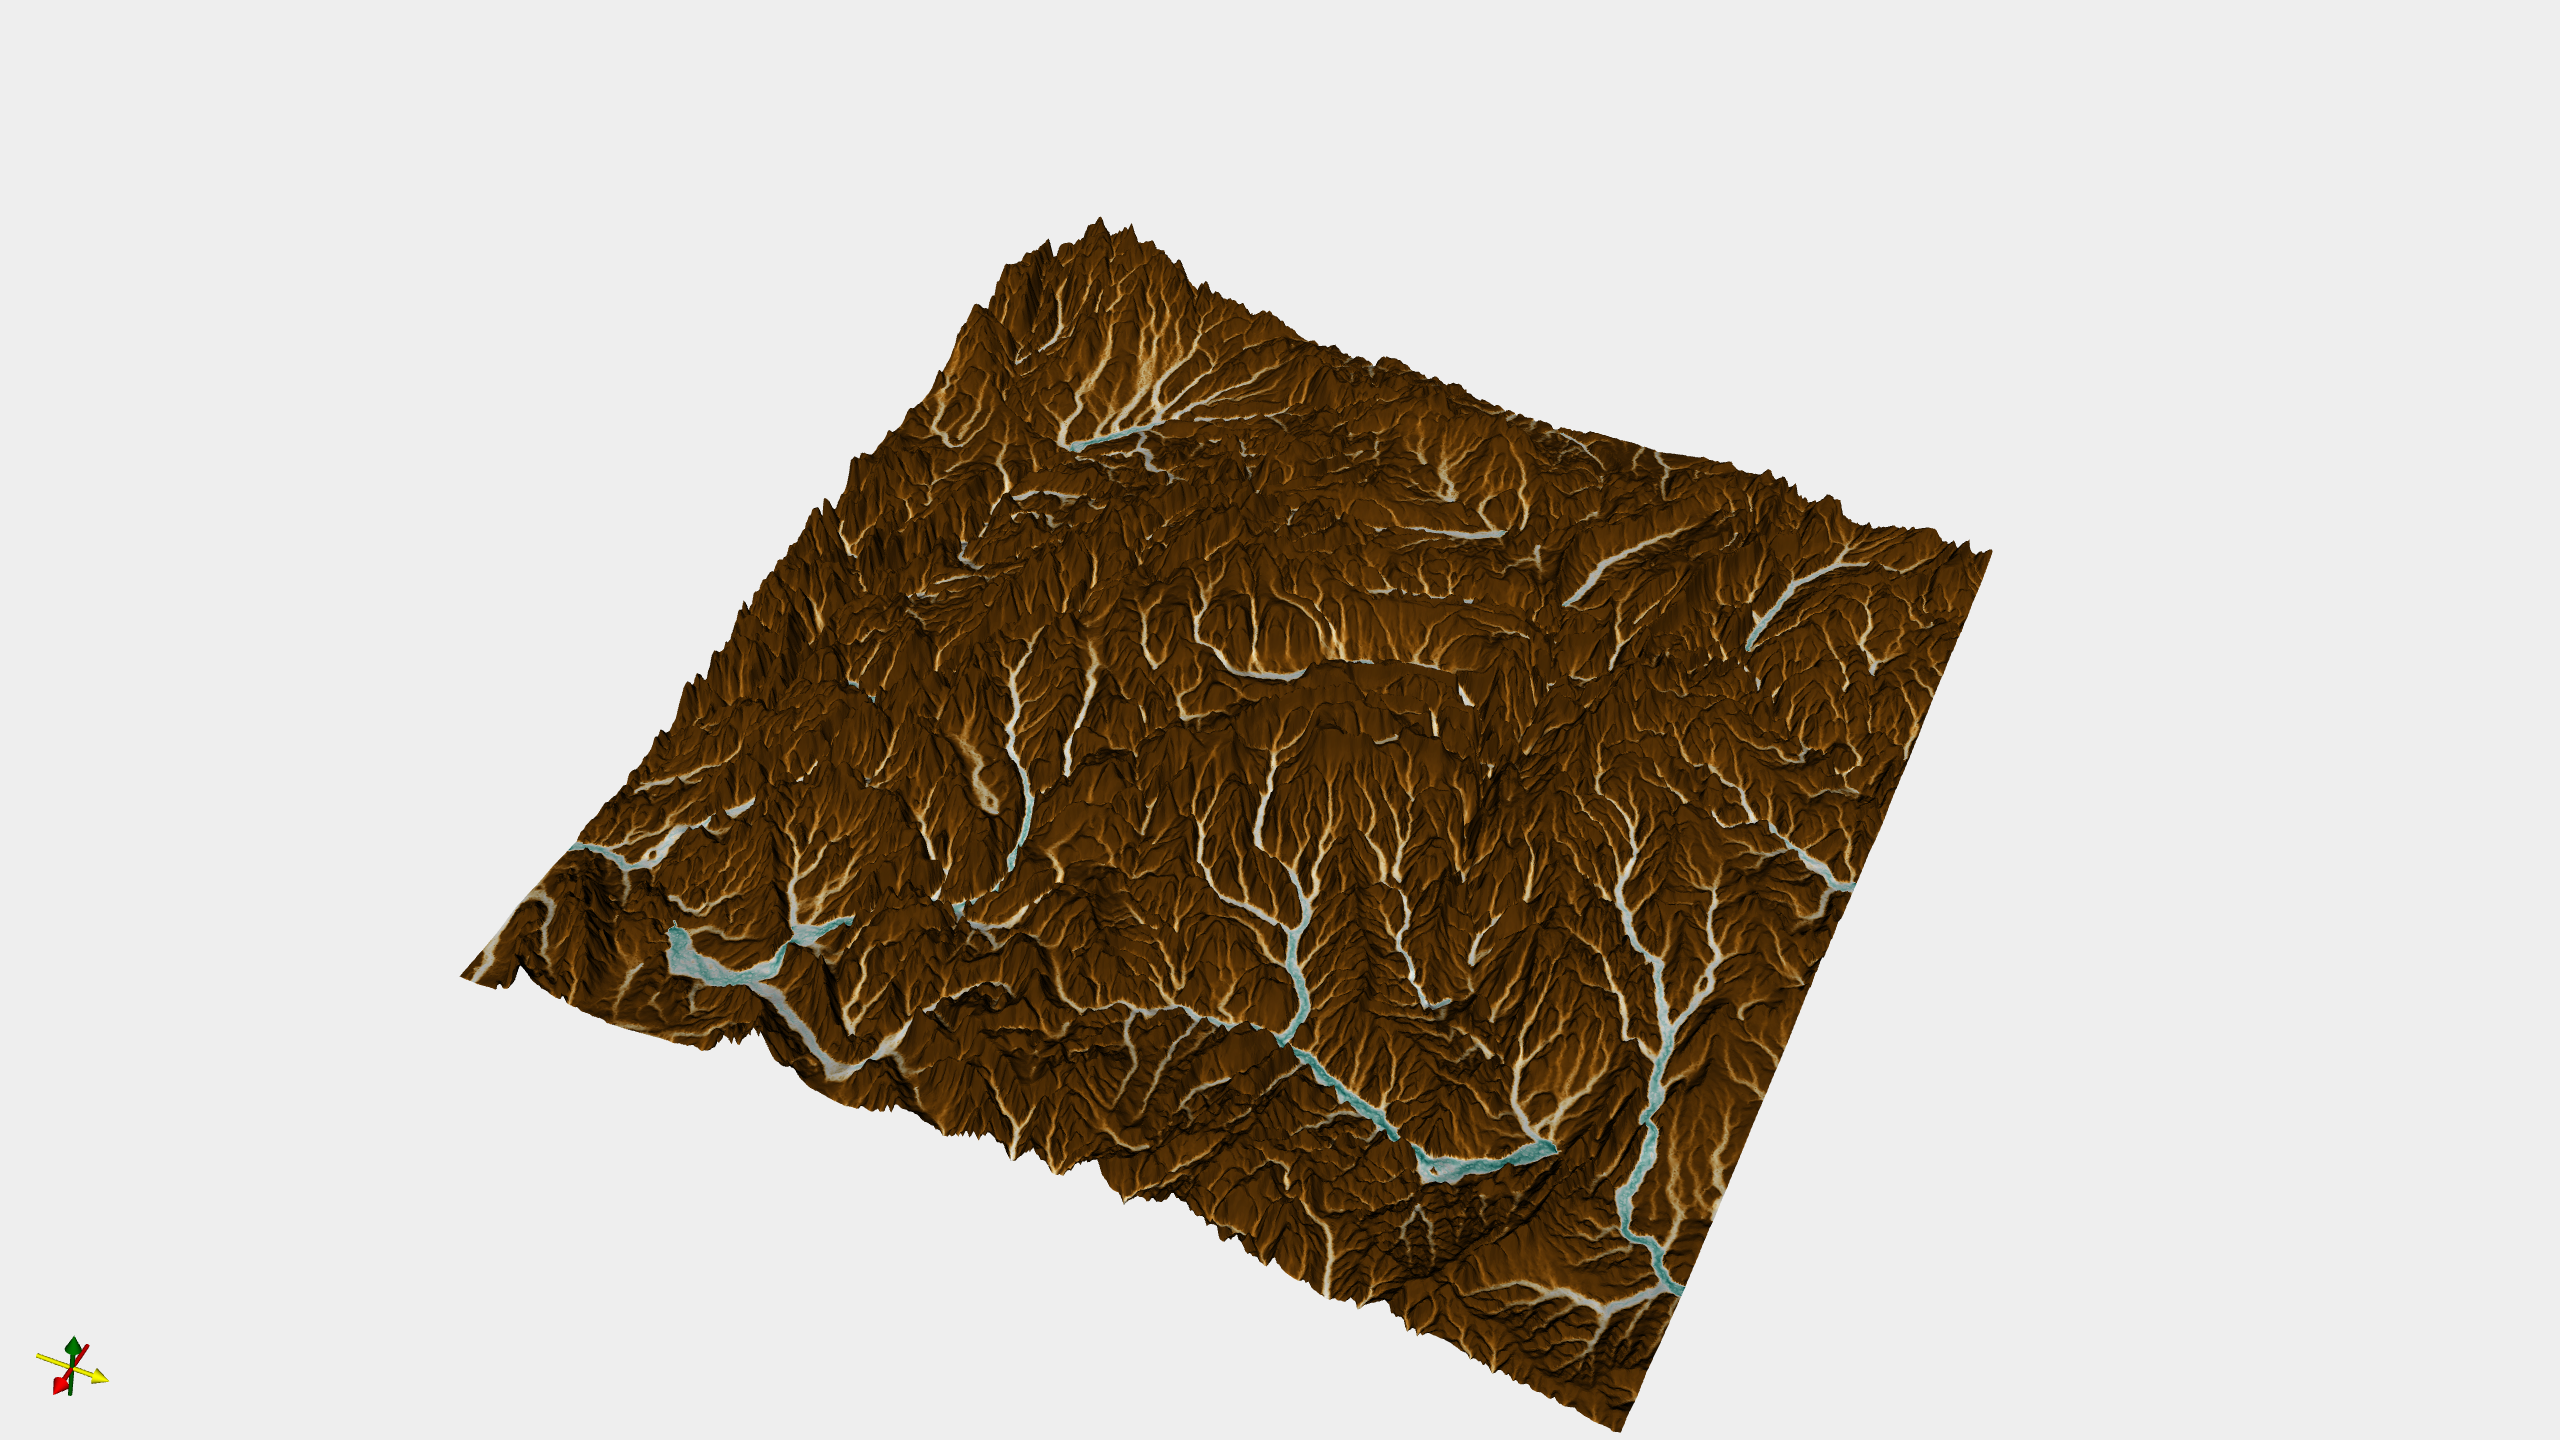
\includegraphics[width=.98\textwidth]{./figures/ch3-bergantes-flow.png}
\end{minipage}
\end{minipage}
\caption{Example model evolution of the Riu Bergantes and surrounding area in the Iberian Massif, Spain. The model fLEM is run on the SRTM (Shuttle Radar Topography Mission) DEM (digital elevation model) that includes the Riu Bergantes in the bottom corner ($40^{\circ}$N,$1^{\circ}$W to $41^{\circ}$N,$0^{\circ}$E). The model is run as described in \cite{armitage-2019} for 20\,kyrs, for which the flow field is displayed on the right. No colour bars are shown, as this model is simply a demonstration of the idea rather than a full simulation.}
\label{fg:bergantes}
\end{figure}

To better understand the key processes I am involved in a large project where we plan to compare multiple LEMs on one single catchment, the Riu Bergantes in Spain (Figure \ref{fg:bergantes}). The aim is to take a series of different LEMs: fLEM \citep{armitage-2019}, TISC \citep{garcia-castellanos-2002}, LAPSUS \citep{schoorl-etal-2000}, and CAESAR-Lisflood \citep{coulthard-etal-2013}, and apply them to the same region and explore how they differ in terms of predicted topography and sediment flux. On a smaller scale, in collaboration with Sébastien Rohais, I am currently exploring how the model fLEM and CAESAR-Lisflood compare for modelling sediment transport within the Southern Gulf of Corinth. Key questions are:
\begin{itemize}
    \item[1] What is the impact of large events vs. long-term low magnitude precipitation? It is often assumed that single large events such as floods lead to significant deposition within the sedimentary record. During the last century for example marine cables have suffered significant damage related to turbidite flows. Are these connected with onshore change in precipitation. The two models can be used to explore how precipitation is recorded at the catchment outlet. The advanteage of fLEM is that calculations are rapid, however the water flux term implicitly assumes a steady state flow. CAESAR-Lisflood uses the Lisflood implementation of non-steady water flux, however run times are long. The two models will be used to explore the immpact of the steady / non-steady water flow.
    \item[2] How sensitive are models to the assumed thickness of transportable regolith? In fLEM it is implicitly assumed that there is an infinate supply of material for transport. However, within CAESAR-Lisflood the depth to bedrock can be defined. How will this control the landscape response?
\end{itemize}
  

\section{Long-Term: Groundwater}

\begin{figure}
    \centering
    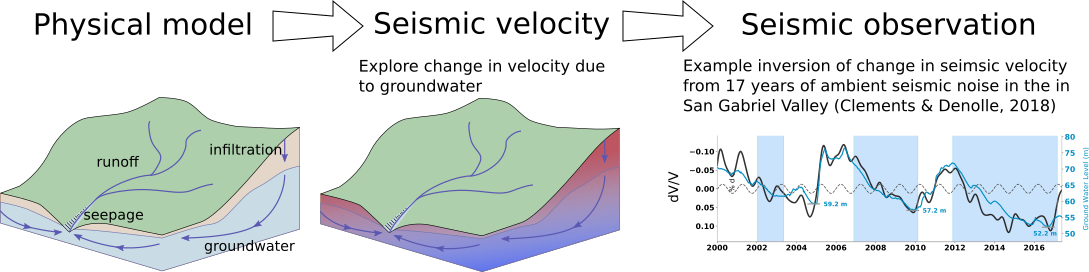
\includegraphics[width=\textwidth]{./figures/groundwater.png}
    \caption{Left: Diagram showing the major interactions between surface run-off and ground-
water. Precipitation is either routed down slope as surface water, or infiltrates into the
critical zone and deeper groundwater reservoirs. Here it can return to the surface as seepage
into the river network. Middle: The hypothetical conversion of physical properties into seismic paramters. Right: Figure from \cite{clements-2018}: Relating seismic wave speed temporal perturbation to ground water levels. Observed $dv/v$ stacked over all station pairs (black) with modeled $dv/v$ due to thermoelastic strain (dashed) removed compared with groundwater change (blue) in the Baldwin Park Key Well. Grey bars indicate lowest historical water levels of the Baldwin Park Key Well. Blue patches indicate times of drought.}
    \label{fg:groundwater}
\end{figure}

The flow of water is the primary mechanism that transports sediment, weathers rocks and leads to landscape change. Water flows across the surface of the ground in streams and rivers, yet this is only a small proportion of the flow of water. The majority of precipitation infiltrates into the subsurface and flows through the ground from mountain catchments to the river. There are two water worlds, surface water and groundwater (Figure \ref{fg:groundwater}). It is often assumed that erosion is driven by the flow of surface water, and groundwater is ignored within numerical models of landscape evolution (landscape evolution models or LEMs). However recent monitoring of groundwater flow in catchments within for example the Himalayas and Taiwan shows that in fact the main rivers are supplied by groundwater, and this system responds on a timescale that is decoupled from the storm driven rainfall input.

I aim to close these two worlds, and develop the methods to include groundwater flow within LEMs. This is not trivial because the flow of water through variably saturated ground involves solving the non-linear Richards' equation. The challenge is to find the acceptable simplifications that create a solvable system of equations and capture the observed response of groundwater to change in precipitation. This challenge can be met due to recent observations of groundwater with ambient seismic noise. The cross-correlation of seismic noise gives a measure of the change in saturation of the subsurface through time. In the Himalayas this has been used to create a three year continuous history of groundwater flow related to two monsoon cycles. Therefore in this project we will develop a reduced complexity model of groundwater flow that is validated against state-of-the-art observations.

As climate changes it is possible that mountainous catchments will receive increased precipitation and that glaciers will melt at an increasing rate. This surface water will enter the subsurface and impact erosion within the valleys. The impact of this water on aquifer recharge and landscape use is difficult to predict in part because there does not yet exist the tools to model their impact. This project would be a first step to field verified modelling of groundwater coupled to a landscape evolution model. The objectives are:
\begin{itemize}
    \item[1] Develop a reduced complexity model of groundwater flow through the saturated and non-saturated subsurface.
    \item[2] Verify the model against seismic observations of groundwater flow.
\end{itemize}

\subsection{Groundwater and surface water}

The majority of precipitation that falls on the Earth’s surface infiltrates into the vadose zone, the region of the subsurface between the surface and the saturated groundwater reservoir. It then either flows laterally within the upper region of this zone as run-off, is taken up within the soil by organic matter and evaporates (evapotranspiration), or enters the groundwater system. Groundwater then enters the river as a baseflow. The baseflow has, for example, been observed to make up to 37\,\% of the water entering the Liwu River in Taiwan \citep{calmels-etal-2011}. This groundwater is separated between a deep reservoir and a more shallow pathway where the water flows through the upper subsurface (often called the critical zone). These pathways are measured from the major element composition of water, which shows three distinct sources, fast run-off, slow run-off and deep groundwater.

Fast run-off has been traditionally captured in LEMs using a simplification of the shallow water equations. One very popular implementation of this fast run-off driven LEM is Caesar-Lisflood, which is suitable for modelling systems over timescales of decades to centuries \citep{coulthard-etal-2013}. Field observations would suggest that this sort of model captures only two thirds of the water flow, as baseflow is not captured. Hydrological models such as ParFlow solve Richards' equation for the flow of water through variably saturated ground, and therefore can capture the slow run-off and deep groundwater \citep[e.g.][]{jones-2001,maxwell-etal-2015}. Yet, there have been limited efforts in connecting the impact of run-off and groundwater on landscape evolution (c.f.\ Penn State Integrated Hydrologic Model, PIHM; \citep{zhang-etal-2016}. More importantly, the few hydrological models that include subsurface flow have not been compared against field measures of the response of groundwater to change in precipitation.
In this project we will explore the impact of assumptions on the relationship between permeability, saturation, and connectivity on the groundwater flow. Furthermore, there are two key sinks for groundwater, baseflow and evapotranspiration. These two sinks will affect how the system responds to a change in precipitation and infiltration. The key to understanding the role of the two sinks in the groundwater flow is the comparison of model simulations to observations.

\subsection{Simulations to observations}

Groundwater elevation can be measured directly from boreholes. Repeat measurements through time can give an indication of the response of the groundwater system to change in climatic conditions. Continuous monitoring of groundwater levels is possible from the cross-correlation of ambient seismic noise (Figure \ref{fg:groundwater}; \citealp{lecocq-etal-2017,clements-2018}). The saturation of the subsurface changes the seismic properties of the subsurface such that the temporal difference in seismic noise can be used to track change in groundwater saturation. In steep mountain catchments there is evidence that the majority of water enters the river systems via baseflow \citep{jasechko-etal-2016}. Furthermore, as climate changes and glaciers continue to melt, this melt water may increasingly enter the groundwater system rather than entre the river systems directly as run-off \citep{vincent-etal-2019}. Recent work from the Bothe Koshi catchment in the Himalayas would suggest the groundwater responds to monsoon precipitation in two steps, a rapid loss of groundwater due to baseflow post monsoon and a slow loss of groundwater due to evapotranspiration \citep{illien-etal-2020}.

\begin{figure}
    \centering
    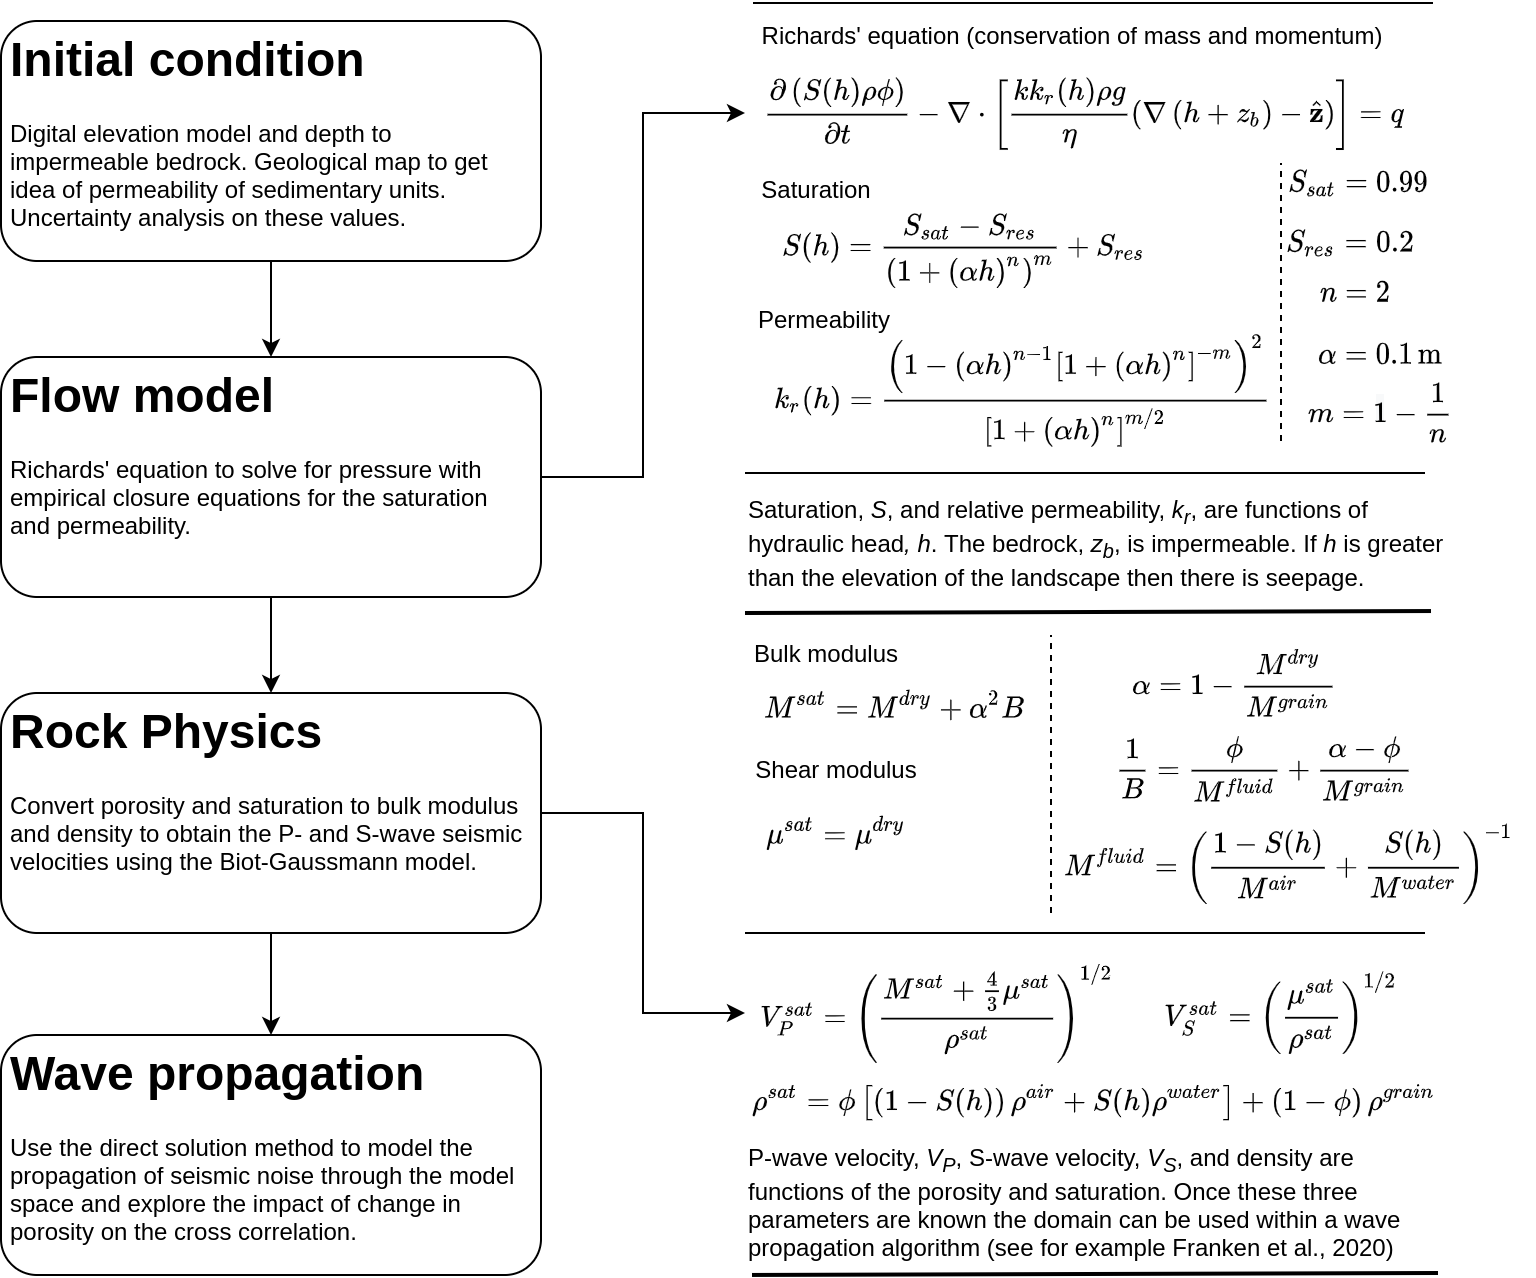
\includegraphics[width=\textwidth]{./figures/groundwater-flowchart.png}
    \caption{Flow diagram for forward modelling the seismic response to groundwater movement. On the left is a simplified step by step flow chart that describes the four main processes, (1) treating the input data, (2) developing the flow model, (3) converting the physical parameters to seismic parameters, (4) wave propagation. On the right are the main model equations that need to be solved for the flow and rock physics. There is once central unknown, the hydraulic head, which then gives the saturation and permeability.}
    \label{fg:groundwater-flowchart}
\end{figure}

Non-invasive measure of groundwater levels can be used to verify models of groundwater transport. Rather than interpret the seismic signal, in this project we will build on methods developed for melt flow within the subsurface \citep{franken-etal-2020,armitage-etal-grl-2019} to explore how a model derived synthetic noise cross-correlation is affected by model assumptions of the effects of surface to subsurface water transport (Fiugre \ref{fg:groundwater-flowchart}). The synthetic model space will be converted from physical properties to seismic P and S-wave velocity as a function of saturation and porosity. Using a Biot-Gassmann theory for the effect of three phases, air, water, and solid grains, the seismic velocities can be estimated from the bulk and shear moduli, and density \citep[e.g.][]{rasolofasaon-2012}. This will allow for the forward conversion of physical properties to seismic properties for the forward propagation of seismic waves through the model domain. The synthetic response of ambient seismic noise cross-correlation can then be compared for different model assumptions.

\subsection{Groundwater observations}

A key aspect of this project is to compare the model synthetics to observations. Variations in the seismic velocity with time, $dV/V$, are derived from an inversion algorithm \citep[e.g.][]{lecocq-etal-2017,clements-2018}. There is a significant layer of preprocessing that is applied to the seismic arrivals prior to the inversion. In oreder to compare synthetic models against observations it is therefore important to use the same processing (as I have done for projects relating to mantle-scale seismic tomography and receiver functions, see for example \citealp{goes-etal-2012,armitage-etal-2015,civiero-etal-2019}). At GFZ in Potsdam, Niels Hovius has lead projects within the Boshi Kosi catchment, Nepal (Himalayas). From three years of continuous monitoring, the groundwater response to two monsoon seasons has been inverted \citep{illien-etal-2020}. Therefore in collaboration with GFZ I propose to explore how the forward model compares to the seismic observations.


%%%%%%%%%%%%%%%%%%%%%%%%%%%%%%%%%%%%%%%%%
% Wilson Resume/CV
% Structure Specification File
% Version 1.0 (22/1/2015)
%
% This file has been downloaded from:
% http://www.LaTeXTemplates.com
%
% License:
% CC BY-NC-SA 3.0 (http://creativecommons.org/licenses/by-nc-sa/3.0/)
%
%%%%%%%%%%%%%%%%%%%%%%%%%%%%%%%%%%%%%%%%%

%----------------------------------------------------------------------------------------
%	PACKAGES AND OTHER DOCUMENT CONFIGURATIONS
%----------------------------------------------------------------------------------------

%\usepackage[a4paper, hmargin=25mm, vmargin=30mm, top=20mm]{geometry} % Use A4 paper and set margins

%\usepackage{fancyhdr} % Customize the header and footer

%\usepackage{lastpage} % Required for calculating the number of pages in the document

%\usepackage{hyperref} % Colors for links, text and headings

\setcounter{secnumdepth}{0} % Suppress section numbering

%\usepackage[proportional,scaled=1.064]{erewhon} % Use the Erewhon font
%\usepackage[erewhon,vvarbb,bigdelims]{newtxmath} % Use the Erewhon font
%\usepackage[utf8]{inputenc} % Required for inputting international characters
%\usepackage[T1]{fontenc} % Output font encoding for international characters

%\usepackage{fontspec} % Required for specification of custom fonts
%\setmainfont[Path = ./fonts/,
%Extension = .otf,
%BoldFont = Erewhon-Bold,
%ItalicFont = Erewhon-Italic,
%BoldItalicFont = Erewhon-BoldItalic,
%SmallCapsFeatures = {Letters = SmallCaps}
%]{Erewhon-Regular}

%\usepackage{color} % Required for custom colors
\definecolor{slateblue}{rgb}{0.17,0.22,0.34}

%\usepackage{sectsty} % Allows customization of titles
%\sectionfont{\color{slateblue}} % Color section titles

%\fancypagestyle{plain}{\fancyhf{}\cfoot{\thepage\ of \pageref{LastPage}}} % Define a custom page style
%\fancypagestyle{plain}{\fancyhf{}\cfoot{\thepage}} % Define a custom page style
%\pagestyle{plain} % Use the custom page style through the document
\renewcommand{\headrulewidth}{0pt} % Disable the default header rule
\renewcommand{\footrulewidth}{0pt} % Disable the default footer rule

\setlength\parindent{0pt} % Stop paragraph indentation

% Non-indenting itemize
\newenvironment{itemize-noindent}
{\setlength{\leftmargini}{0em}\begin{itemize}}
{\end{itemize}}

% Text width for tabbing environments
\newlength{\smallertextwidth}
\setlength{\smallertextwidth}{\textwidth}
\addtolength{\smallertextwidth}{-2cm}

\newcommand{\sqbullet}{~\vrule height 1ex width .8ex depth -.2ex} % Custom square bullet point definition

%----------------------------------------------------------------------------------------
%	MAIN HEADER COMMAND
%----------------------------------------------------------------------------------------

\renewcommand{\title}[1]{
{\huge{\color{slateblue}\textbf{#1}}}\\ % Header section name and color
\rule{\textwidth}{0.5mm}\\ % Rule under the header
}

%----------------------------------------------------------------------------------------
%	JOB COMMAND
%----------------------------------------------------------------------------------------

\newcommand{\job}[6]{
\begin{tabbing}
\hspace{2cm} \= \kill
\textbf{#1} \> \href{#4}{#3} \\
\textbf{#2} \>\+ \textit{#5} \\
\begin{minipage}{\smallertextwidth}
\vspace{2mm}
#6
\end{minipage}
\end{tabbing}
\vspace{2mm}
}

%----------------------------------------------------------------------------------------
%	SKILL GROUP COMMAND
%----------------------------------------------------------------------------------------

\newcommand{\skillgroup}[2]{
\begin{tabbing}
\hspace{5mm} \= \kill
\sqbullet \>\+ \textbf{#1} \\
\begin{minipage}{\smallertextwidth}
\vspace{2mm}
#2
\end{minipage}
\end{tabbing}
}

%----------------------------------------------------------------------------------------
%	INTERESTS GROUP COMMAND
%-----------------------------------------------------------------------------------------

\newcommand{\interestsgroup}[1]{
\begin{tabbing}
\hspace{5mm} \= \kill
#1
\end{tabbing}
\vspace{-10mm}
}

\newcommand{\interest}[1]{\sqbullet \> \textbf{#1}\\[3pt]} % Define a custom command for individual interests

%----------------------------------------------------------------------------------------
%	TABBED BLOCK COMMAND
%----------------------------------------------------------------------------------------

\newcommand{\tabbedblock}[1]{
\begin{tabbing}
\hspace{2cm} \= \hspace{4cm} \= \kill
#1
\end{tabbing}
}

%----------------------------------------------------------------------------------------
%	PUBLICATION COMMAND
%----------------------------------------------------------------------------------------

\newcommand{\pub}[2]{
\begin{tabbing}
\hspace{2cm} \= \kill
\textbf{#1} \>
\begin{minipage}{\smallertextwidth}
\vspace{.5mm}
#2
\end{minipage}
\end{tabbing}
\vspace{.5mm}
}
 
%%%%%%%%%%%%%%%%%%%%%%%%%%%%%%%%%%%%%%%%%
% Wilson Resume/CV
% XeLaTeX Template
% Version 1.0 (22/1/2015)
%
% This template has been downloaded from:
% http://www.LaTeXTemplates.com
%
% Original author:
% Howard Wilson (https://github.com/watsonbox/cv_template_2004) with
% extensive modifications by Vel (vel@latextemplates.com)
%
% License:
% CC BY-NC-SA 3.0 (http://creativecommons.org/licenses/by-nc-sa/3.0/)
%
%%%%%%%%%%%%%%%%%%%%%%%%%%%%%%%%%%%%%%%%%

\chapter{Rèsumé}

%----------------------------------------------------------------------------------------
%	EDUCATION SECTION
%----------------------------------------------------------------------------------------

\section{Education}

\tabbedblock{
\bf{2004-2009} \> PhD in Geophysics - National Oceanography Centre, University of Southampton, UK \\[5pt]
\>Title `How Does Melting Affect Continental Rift Development?' \\
\>Supervisors: Prof Tim Minshull, Dr Tim Henstock \& Dr John Hopper\\
\>\+
\textit{Awarded a fully funded NERC studentship}
}

%------------------------------------------------

\tabbedblock{
\bf{2003-2004} \> Masters in Oceanography - National Oceanography Centre, University of Southampton, UK \\[5pt]
\>Masters Project Title `Dissolution of Silica from Antarctic Continental Shelf Sea Sediments'\\ \>Supervisor: Prof. Rachel Mills\\
\>\+
\textit{Awarded a fully funded NERC scholarship}
}

%------------------------------------------------

\tabbedblock{
\bf{1999-2003} \> MSci in Physics - Imperial College London, UK \\%[5pt]
%\>Upper Second Class Honours- 79\% Average\\
\>\+
}

%----------------------------------------------------------------------------------------
%	EMPLOYMENT HISTORY SECTION
%----------------------------------------------------------------------------------------

\section{Employment History}

\job
{Feb 2020 -}{Present}
{IFP Energies Nouvelles}
{http://www.ifpenergiesnouvelles.fr}
{Ingènieur de Recherche}
{}

%------------------------------------------------

\job
{Oct 2019 -}{Feb 2020}
{Gekko SAS, Paris, France}
{http://www.gekko.fr}
{Cloud Computing and DevOps Consultant}
{}

%------------------------------------------------

\job
{Sep 2015 -}{Aug 2019}
{Institut de Physique du Globe de Paris, France}
{http://www.ipgp.fr}
{ANR Funded Research Scientist}
{I was the principle investigator on a prestigious 4 year Agence National de la Recherche funded grant through the “Acceuil de Chercheurs de Haut Niveau” call.}

%------------------------------------------------

\job
{Sep 2013 -}{Aug 2015}
{Department of Earth Sciences, Royal Holloway, University of London, UK}
{https://www.royalholloway.ac.uk/earthsciences/home.aspx}
{Royal Astronomical Society Research Fellow}
{This fellowship, titled “Deciphering the sedimentary record: tectonic vs climate change”, was awarded by the Royal Astronomical Society. I explored how long-wavelength topography changes due to mantle flow, and whether long lived changes in climate have affected the sedimentary record of continental interiors I am continuing collaborations with Prof.~Jason Phipps Morgan, Prof.~Peter Burgess and Prof.~Marta P{\'e}rez-Gussiny{\'e} to couple numerical models of mantle flow to first order sedimentary processes.}

%------------------------------------------------

\job
{Apr 2011 -}{Aug 2013}
{Institut de Physique du Globe de Paris, France}
{http://www.ipgp.fr}
{Marie Curie Research Fellow}
{This two year EU Marie Curie fellowship was titled “Cratonic basins: an archive of lithosphere-mantle interaction”. Collaborating with Prof.~Claude Jaupart (IPGP); I studied how deep mantle dynamics is recorded in the rock record by exploring the relationship between lithosphere destabilisation and subsidence within the continental interior, with a focus on cratonic basins. The primary aim was to develop my numerical and laboratory experimental skills.}

%------------------------------------------------

\job
{Mar 2008 -}{Mar 2011}
{Department of Earth Science and Engineering, Imperial College London, UK}
{https://www.imperial.ac.uk/earth-science/}
{Research Associate}
{I worked within the Sediment Routing Systems group, headed by Prof. Philip Allen, to (1) Develop models of basin formation and couple models of subsidence with the evolution of grain size. In particular I looked at the possibility of subsidence within the continental interior at cratonic basins being due to a low strain rate extension. (2) Develop models of catchment erosion and sediment deposition to explore the controls of basin stratigraphy due to changes in climate and uplift within the catchment.}

%----------------------------------------------------------------------------------------
%	FUNDING
%----------------------------------------------------------------------------------------

\section{Funding}

\tabbedblock{
\bf{Sep 2015} \> ANR Acceuil de Chercheurs de Haut Niveau 4 year research project \\
\> `InterRift: Interpreting Continental Break-up from Surface Observations' -- 450,000\euro \\
\bf{Aug 2013} \> Royal Astronomical Society Research Fellowship -- \pounds123,000 \\
\bf{Apr 2011} \> E.U.~Marie Curie Research Fellowship -- 193,564\euro \\
}

%----------------------------------------------------------------------------------------
%	AWARDS
%----------------------------------------------------------------------------------------

\section{Awards}

\tabbedblock{
\bf{2011} \> Young Author of the Year, Journal of the Geological Society, London, for the article\\
\> “Cratonic basins and the long-term subsidence history of continental interiors”.\\
\bf{2009} \> Masanori Sakuyama Prize, for best publication of a PhD graduate of the National \\
\> Oceanography Centre, Southampton: `Modelling the composition of melts formed during the\\
\> continental break-up of the North Atlantic', published in Earth and Planetary Science Letters.\\
\bf{2007} \> Best poster at the Faculty of Engineering, Science \& Mathematics Research\\
\> Showcase, University of Southampton.\\
\bf{2003} \> NERC scholarships including living costs for my Masters in Oceanography \& my PhD.\\
}

%----------------------------------------------------------------------------------------
%	PhD SUPERVISION
%----------------------------------------------------------------------------------------

\section{PhD Supervision}

\job
{2016 -}{2019}
{Thijs Franken}
{}
{Institut de Physique du Globe de Paris}
{I was the primary supervisor of Thijs Franken. Thijs' PhD focused on developing models of seismic structure due to partial melt and wave propagation through regional domains.  This project was funded through my ANR grant, and was in collaboration with Dr.~Nobuaki Fuji and Prof.~Alexandre Fournier (IPGP).}

\job
{2014 -}{2018}
{Sam Brooke}
{}
{Imperial College London}
{I co-supervised Sam Brooke with Dr.~Alex Whittaker at Imperial College London. The aim of this project was to further develop models of sediment transport and the evolution of alluvial fans.}

\job
{2012 -}{2017}
{Chandra Taposeea}
{}
{Imperial College London}
{I co-supervised Chandra Taposeea with Dr.~Jenny Collier at Imperial College London. The project further tests the hypothesis developed by myself, Jenny Collier and Tim Minshull (National Oceanography Centre, Southampton) that rift history controls the volume of melt generated during continental break-up.}

%----------------------------------------------------------------------------------------
%	MASTERS SUPERVISION
%----------------------------------------------------------------------------------------
\section{Masters and Undergraduate Supervision}

\tabbedblock{
\bf{2017} \> Masters research project: Aimen Maghrebi, \textit{Ecole Supérieure d’Ingénieurs Léonard de Vinci}.\\
\bf{2017} \> 3rd year undergraduate project: Sabrina Ihaddadene, License, \textit{Physique, Université Paris-Est Créteil}.\\
\bf{2016} \> 3rd year undergraduate project: Leo Bourier, License, \textit{Physique, Université Paris-Est Créteil}.\\
}

%----------------------------------------------------------------------------------------
%	TEACHING
%----------------------------------------------------------------------------------------
\section{Teaching}

\tabbedblock{
\bf{2018} \> Université Paris Diderot, Surface Processes, Masters level, 50h\\
\bf{2017} \> Université Paris Diderot, UE Projet Tutoré, 3rd year undergraduate, 42h\\
\bf{2016} \> Institut de Physique du Globe de Paris, `Frontiers in Earth surface dynamics: creating a\\
\> research proposal', École doctorale (PhD level), 10h\\
\bf{2016} \> Université Pierre et Marie Curie, Séminaire Géodynamique, Masters level, 3h\\
\bf{2014} \> Royal Holloway, University of London, Sedimentary Basin Analysis, 3rd year undergraduate, 6h\\
\bf{2010} \> Imperial College London, Mathematics of Geology and Geophysics, 1st year undergraduate, 20h\\
\bf{2007-2008} \> University of Southampton, Biogeochemical cycles, Masters level, 20h\\
}

%----------------------------------------------------------------------------------------
%	SELECTED CONFERENCE PRESENTATIONS
%----------------------------------------------------------------------------------------

\section{Selected Invited Presentations}

{\bf EGU General Assembly 2018}: From induction to deduction: Using the Earth as a natural laboratory. EGU2018-10469, April, 2018.\\
{\bf Ordinary Meeting of the RAS}: Can variations in the Earth's orbit create stratigraphic sequences? 10th March 2017\\
{\bf Geological Society of London}, Rifts III: Catching the wave, 2016: Upper mantle temperature during extension and breakup, 22-24 March, 2016.\\
{\bf AGU Fall Meeting 2015}: Testing How Depletion, Dehydration and Melt Affect Seismic Expressions of the Asthenosphere, T34C-01, December 16th, 2015.\\
{\bf Volkswagen-Stiftung Funded Symposium}: Bridging the Gap Between Field Evidence and Numerical Models: Modelling landscape and sediment flux responses to precipitation change, Herrenhausen Palace Conference Centre, Hanover, October 21-23rd, 2015.\\
{\bf Action Marges Workshop, Mouvements verticaux et Chantier Afar-Aden}: Keynote: Controls of lithospheric extension on magma and sediment production, Total, La Defence, November 11-12th, 2014.\\
{\bf Volcanic \& Magmatic Studies Group 2012 Conference}: Keynote: Beyond Hotspots: the importance of rift history for volcanic margin formation, Durham University, UK, January 4-6th, 2012.\\
{\bf EarthScope - GeoPRISMS Science Workshop on Eastern North America (ENAM)}: Analogue and numerical models that inform the rifting process, Lehigh University, Bethlehem, PA, USA, October 27-29th, 2011.\\

\section{Selected Oral Conference Presentations}
Armitage, J.J. (2017), The Effect of Climate Change on Volcanism During Continental Break-up, 79th EAGE Conference and Exhibition 2017.\\
Armitage, J.J. (2016), But What About Trees and Beavers? Simplicity, Complexity and Benchmarks for Landscape Evolution Models,  AGU, Fall Meet., Abstract, EP12A-07\\
Armitage, J.J. (2015), Landscape response due to sediment transport and bedrock detachment, GeoBerlin, Dynamic earth – from Alfred Wegener to today and beyond, Berlin.\\
Armitage, J.J. (2014), The influence of large-scale tectonics, mantle flow and climatic change on sediment accumulation, William Smith Meeting 2014: The Future of Sequence Stratigraphy: Evolution or Revolution? The Geological Society, London.\\
Armitage J.J., Barrier, L. (2013), Is the Neogene series of the Northern Foreland Basin of the Tian Shan Range indicative of tectonic or climatic change? AGU, Fall Meet., Abstract EP43E-04 \\
Armitage J.J. (2012), The Instability of Continental Passive Margins and its Effect on Continental Topography and Heat Flow, Deep Water Margins, The Geological Society, London.\\
Goes, S.D., Armitage, J.J., Harmon, N., Huismans, R.S., (2011), Low seismic velocities below mid-ocean ridges: Attenuation vs. melt retention, AGU, Fall Meet., Abstract, T33H-05 \\
Armitage J.J., Duller, R.A., Whittaker, A.C., Densmore, A, Allen, P.A., (2010) Response of sediment routing systems to tectonic and climatic perturbations, William Smith Meeting 2010 - Landscapes Into Rock, The Geological Society, London.\\
Armitage J.J., Collier, J.S., Minshull T.A., Hopper J.R., (2008), Geodynamic modelling of the opening of the northwest Indian Ocean, AGU, Fall Meet., Abstract, T53G-08\\
Armitage J.J., Henstock T.J., Minshull T.A., Hopper J.R., (2007), Lithospheric controls on the rifting of continents at slow rates of extension, AGU, Fall Meet. Suppl., Abstract, T32A-06\\

\section{Invited Seminars}
More than 20 invited seminars since 2012.
\tabbedblock{
\bf{2018} \> University of Leeds \\
\bf{2017} \> ISTerre Grenoble; GET Toulouse; IRAP Toulouse \\
\bf{2016} \> Universié de Lausanne; GFZ Potsdam \\ 
\bf{2015} \> University of Edinburgh; MINES ParisTech; University of Southampton \\
\bf{2014} \> University of Southampton \\
\bf{2013} \> Université de Montpelier; Université de Nantes; Université Paris Sud, Orsay \\
\bf{2012} \> ENS, Paris; FAST, Université Paris Sud, Orsay; CPRG Nancy; UMPC, Paris; Université de Rennes;\\
          \> EOST Strasbourg \\
}

%----------------------------------------------------------------------------------------
%	PUBLICATIONS
%----------------------------------------------------------------------------------------

\section{List of publications}

\pub {36}{ Franken, T, {\bf Armitage, J.J.}, Fuji, N, Fournier, A., (2020) Seismic wave-based constraints on geodynamical processes: an application to partial melting beneath the Réunion island. Geochemistry, Geophysics, Geosystems, doi: TBA}

\pub {35}{ Civiero, C., {\bf Armitage, J.J.}, Goes, S., Hammond, J.O.S., (2019) The seismic signature of upper‐mantle plumes: application to the northern East African Rift. Geochemistry, Geophysics, Geosystems, 20, 6106-6122, doi: 10.1029/2019GC008636}
\pub {34}{ Andrés-Mart\'inez, M., Pérez-Gussinyé, M., {\bf Armitage, J.J.}, Morgan, J.P., (2019) Thermomechanical implications of sediment transport for the architecture and evolution of continental rifts and margins. Tectonics, 38, 641-665, doi: 10.1029/2018TC005346}
\pub {33}{ Duller, R.A., {\bf Armitage, J.J.}, Manners, H.R., Grimes, S., Jones, T.D., (2019) Delayed sedimentary response to abrupt climate change at the Paleocene-Eocene boundary, northern Spain. Geology, 47, 159-162, doi: /10.1130/G45631.1}
\pub {32}{ {\bf Armitage, J.J.} (2019) Short communication: flow as distributed lines within the landscape. Earth Surface Dynamics, 7, 67-75, doi: 10.5194/esurf-7-67-2019}
\pub {31}{ {\bf Armitage, J.J.}, Ferguson, D.J., Petersen, K.D., Creyts, T.T., (2019) The importance of Icenlandic ice sheet growth and retreat on mantle CO$_2$ flux. Geophyscial Research Letters, 46, 6451-658, doi: 10.1029/2019GL081955}
\pub {30}{ {\bf Armitage, J.J.}, Collier, J.S., (2017) The thermal structure of volcanic passive margins. Petroleum Geoscience, 24, 393-401, doi: 10.1144/petgeo2016-101}
\pub {29}{ Brooke, S.A.S., Whittaker, A.C., {\bf Armitage, J.J.}, D'Arcy, M., Watkins, S.E., (2018) Quantifying sediment transport dynamics on alluvial fans from spatial and temporal changes in grain size, Death Valley, California. Journal of Geophysical Research -- Earth Surface, 123, 2039-2067, doi: 10.1029/2018JF004622}
\pub {28}{ Rychert, C.A., Harmon, N., {\bf Armitage, J.J.}, (2018) Seismic imaging of thickened lithosphere resulting from plume pulsing beneath Iceland. 19, 1789-1799, doi: 0.1029/2018GC007501}
\pub {27}{ {\bf Armitage, J.J.}, Petersen, K.D., Perez-Gussinye, M., (2018) The role of crustal strength in controlling magmatism and melt chemistry during rifting and break-up. Geochemistry Geophysics Geosystems, doi: 10.1002/2017GC007326}
\pub {26}{ {\bf Armitage, J.J.}, Burgess, P.M.,  Hampson, G.J., Allen, P.A., (2018) Deciphering the origin of cyclical gravel front and shoreline progradation and retrogradation in the stratigraphic record. Basin Research, 30, 15-35, doi: 10.1111/bre.12203}
\pub {25}{ {\bf Armitage, J.J.}, Whittaker, A.C., Zakari, M., Campforts, B., (2018) Numerical modelling landscape and sediment flux response to precipitation rate change. Earth Surface Dynamics, 6, 77-99, doi: 10.5194/esurf-6-77-2018}
\pub {24}{ Taposeea, C.A., {\bf Armitage, J.J.}, Collier, J.S., (2017) Asthenosphere and lithosphere structure controls on early onset oceanic crust production in the southern South Atlantic. Tectonophysics, 716, 4-20, doi 10.1016/j.tecto.2016.06.026}
\pub {23}{ Mareschal, J.-C., Jaupart, C., {\bf Armitage, J.J.}, Phaneuf, C., Pickler, C.,  Bouquerel, H., (2017) The Sudbury Huronian Heat Flow Anomaly, Ontario, Canada. Precambrian Research, 295, 187-202, doi: 0.1016/j.precamres.2017.04.024}
\pub {22}{ Allen, P.A., Michael, N.A., D’Arcy M., Roda-Boluda, D.C., Whittaker, A.C., Duller, R.A, {\bf Armitage, J.J.}, (2017) Fractionation of grain size in terrestrial sediment routing systems. Basin Research, 29, 180-202, doi: 10.1111/bre.12172}
\pub {21}{ Temme, A.J.A.M., {\bf Armitage, J.J.}, Attal, M., van Gorp, W., Coulthard, T.J., Schoorl, J.M., (2017) Developing, choosing and using landscape evolution models to inform field-based landscape reconstruction studies. Earth Surface Processes and Landforms, 42, 2167–2183, doi: 10.1002/esp.416}
\pub {20}{ Duller, R.A., Warner, N.H., De Angelis, S., {\bf Armitage, J.J.}, Poyatos-More, M., (2015) Reconstructing the timescale of a catastrophic fan-forming event on Earth using a Mars model. Geophysical Research Letters, 42, 10324-10332, doi: 10.1002/2015GL066031}
\pub {19}{ {\bf Armitage, J.J.}., Allen, P. A., Burgess, P. M., Hampson, G. J., Whittaker, A. C., Duller, R. A., Michael, N. A., (2015) Physical stratigraphic model for the Eocene Escanilla sediment routing system: Implications for the uniqueness of sequence stratigraphic architectures. Journal of Sedimentary Research, 85, 1510-1524, doi:10.2110/jsr.2015.97}
\pub {18}{ Allen, P.A., {\bf Armitage, J.J.}, Whittaker, A.C., Michael, N.A., Roda-Boluda, D., D’Arcy, M., (2015) Fragmentation model of the grain size mix of sediment supplied to basins. Journal of Geology, 123, 405-427, doi: 10.1086/683113}
\pub {17}{ {\bf Armitage, J.J.}, Ferguson D., Goes, S., Hammond, J.O.S., Calais, E., Harmon, N., Rychert, C.A., (2015) Upper mantle temperature and the onset of extension and break-up in Afar, Africa. Earth and Planetary Science Letters, 418, 78-90, doi: 10.1016/j.epsl.2015.02.039}
\pub {16}{ Lucazeau, F., {\bf Armitage, J.J.}, Kadima Kabongo, E., (2015) Thermal regime and evolution of the intracratonic Congo Basin, in The Geology and Resource Potential of the Congo Basin , de Wit, M.J., Guillocheau, F., Fernadez-Alonso, M., Kanda, N., and de Wit, M.C.J., Eds. Elsevier. doi: 10.1007/978-3-642-29482-2\_12}
\pub {15}{ Petersen, K.D., {\bf Armitage, J.J.}, Nielsen, S.B., Thybo, H., (2015) Mantle temperature as primary control on the time scale of thermal evolution of extensional basins, Earth and Planetary Science Letters, 409, 61-70, doi: 10.1016/j.epsl.2014.10.043}
\pub {14}{ {\bf Armitage, J.J.}, Duller, R.A., Schmalholz, S.M., (2014) The influence of long-wavelength tilting and climatic change on sediment accumulation. Lithosphere, 6, 303-318, doi: 10.1130/L343.1}
\pub {13}{ {\bf Armitage, J.J.}, Dunkley Jones, T., Duller, R.A., Whittaker, A.C., Allen, P.A., (2013) Temporal buffering of climate-driven sediment flux cycles by transient catchment response. Earth and Planetary Science Letters, 369, 200-210, doi: 10.1016/j.epsl.2013.03.020}
\pub {12}{ {\bf Armitage, J.J.}, Jaupart, C., Fourel, L., Allen, P.A. (2013) The instability of continental passive margins and its effect on continental topography and heat flow. Journal of Geophysical Research – Solid Earth, 118, 1817–1836, doi: 10.1002/jgrb.50097}
\pub {11}{ Allen, P.A., {\bf Armitage, J.J.}, Carter, A., Duller, R.A., Michael, N., Sinclair, H.D., Whitchurch, A.L., Whittaker, A.C. (2013) The Qs problem: Sediment mass balance of proximal foreland basin systems. Sedimentology, 60, 102-130, doi: 10.1111/sed.12015}
\pub {10}{ Goes, S., {\bf Armitage, J.J.}, Harmon, N., Smith, H., Huismans, R., (2012) Low seismic velocities below mid-ocean ridges: Attenuation vs. melt retention. Journal of Geophysical Research – Solid Earth, 117(B12403), doi: 10.1029/2012JB009637}
\pub {9}{ Duller, R.A., Whittaker, A.C., Swinehart, J.B., {\bf Armitage, J.J.}, Sinclair, H.D., Bair, A.R., Allen, P.A., (2012) Abrupt landscape change post-6 Ma on the Central Great Plains, U.S.A. Geology, 40, 871-874}
\pub {8}{ Allen, P.A. \& {\bf Armitage, J.J.}, (2012) Cratonic basins. In Busby, C. \& Azor, A. (Eds.) Syntectonic Basin Development, Active to Ancient: Recent Advances. Ch. 30, p 602-620, Blackwell Publishing Ltd.}
\pub {7}{ {\bf Armitage, J.J.}, Warner, N.H., Goddard, K., Gupta, S., (2011) Timescales of alluvial fan development on Mars. Geophysical Research Letters , 38 (L17203), doi:10.1029/2011GL048907}
\pub {6}{ {\bf Armitage, J.J.}, Collier, J.S., Minshull, T.A. Henstock, T.J. (2011) Thin oceanic crust and flood basalts: Reconciling observations from the northwest Indian Ocean. Geochemistry Geophysics Geosystems, 12(Q0AB07), doi:10.1029/2010GC003316}
\pub {5}{ {\bf Armitage, J.J.}, Duller, R.A., Whittaker, A.C. Allen, P.A., (2011) Transformation of tectonic and climatic signals from source to sedimentary archive. Nature Geoscience, 4, 231-235, doi: 10.1038/ngeo1087}
\pub {4}{ {\bf Armitage, J.J.} \& Allen, P.A. (2010) Cratonic basins and the long-term subsidence history of continental interiors. Journal of the Geological Society, London, 167, 61-70, doi: 10.1144/0016-76492009-108}
\pub {3}{ {\bf Armitage, J.J.}, Collier, J.S., Minshull, T.A., (2010) The importance of rift history for volcanic margin formation. Nature, 465, 913-917, doi: 10.1038/nature09063}
\pub {2}{ {\bf Armitage, J.J.}, Henstock, T.J., Minshull, T.A., Hopper, J.R.,  (2009) Lithospheric controls on melt production during continental breakup at slow rates of extension: Application to the North Atlantic. Geochemistry Geophysics Geosystems, 10(Q06018), doi: 10.1029/2009GC002404}
\pub {1}{ {\bf Armitage, J.J.}, Henstock, T.J., Minshull, T.A., Hopper, J.R., (2008) Modelling the composition of melts formed during continental break-up of the North Atlantic. Earth Planetary Science Letters, 269, 248-258, doi: 10.1016/j.epsl.2008.02.024}



\appendix
\chapter{Example Publications Part 1: Mantle}

In this appendix I have selected five key publications from my research carear that exemplify my apporach and collaborations for understanding how upper mantle processes are reflected in surface observations, and how these processes interact to control how the Earth has evolved.

\begin{itemize}

\item[1] {\bf The importance of rift history for volcanic margin formation -- Nature}

The first paper was published in Nature in 2010 a year after completion of my thesis and represents the culmination of four years work with Tim Minshull and Jenny Collier. In this article we present the hypothesis that lithosphere strucutre controls volcanism during continental break-up. This is expressed by the different evolution of crustal thickness at two classic volcanic margins, the North Atlantic Igneous Provinc and the Seychelles, Laxmi Ridge and Deccan Traps.

\item[2] {\bf Upper mantle temperature and the onset of extension and break-up in Afar, Africa -- Earth and Planetary Science Letters}

In this study I aimed to reconicle diverging interpretations on the structure of the mantle below Afar. Based on teh igneous geochemistry, researchers had reasoned that the upper mantle below Afar must be hot, very hot. However, seismic observations pointed to the mantle being not cold, or at least not hotter than average. I developed the methods to predict simultaneously the igneous geochemistry and seismic structure to demonstrate, that within observatial error, the mantle below Afar is hotter than average.

\item[3] {\bf Thermomechanical implications of sediment transport for the architecture and evolution of continental rifts and margins -- Tectonics}

This study comes from a collaboration I was involved in while working at Royal Holloway, University of London. I worked closely with Miguel Andrés-Mart\'inez to develop a coupled model of surface and shallow mantle processes. This model is the first to fully couple sedimentary processes with crustal deformation. In this study Miguel demonstrates that sediment deposition will alter the evolution of rifted basins. More importantly, geologic interpretation of sedimentary layers is over simplstic, with sediment sourced from one margin ending up on the other after break-up.

\item[4] {\bf The importance of Icelandic ice sheet growth and retreat on mantle CO$_2$ flux -- Geophyscial Research Letters}

Noting that surface processes has a key role in break-up, in collaboration with various colleagues, I beccame interested in how ice-sheet loading might have impacted melt migration and retention. In this study I developed a simple 1D model of melt migration and composition. This allowed the classic hypotheses that Holocene deglaciation caused increased volcanism in Iceland. In this interdisciplineary collaboration, we demonstrated with a range of geological observations, that this hypothesis is most likely true.

\item[5] {\bf Seismic Wave-Based Constraints on Geodynamical Processes: An Application to Partial Melting Beneath the Réunion Island}

The final paper in this set is the work of my former PhD student Thijs Franken in collaboration with Nobuaki Fuji and Alexandre Fournier. This publication is the first attempt at developing a fully forward model to predict the seismic waveform from first principles. A 1D model of melt migration was used to predict the seismic velocity structure below La Réunion. This model then was embedded within a 1D Earth model. Seismic waves were then propagated through the model domain allowing for the comparison of synthetic arrivals against observed seismic arrivals at the RER station on La Réunion. Based on comparisons between the synthetic waveforms and hte observations we found that melt retention is likely low below La Reunion and melt transport rates are high.

\end{itemize}

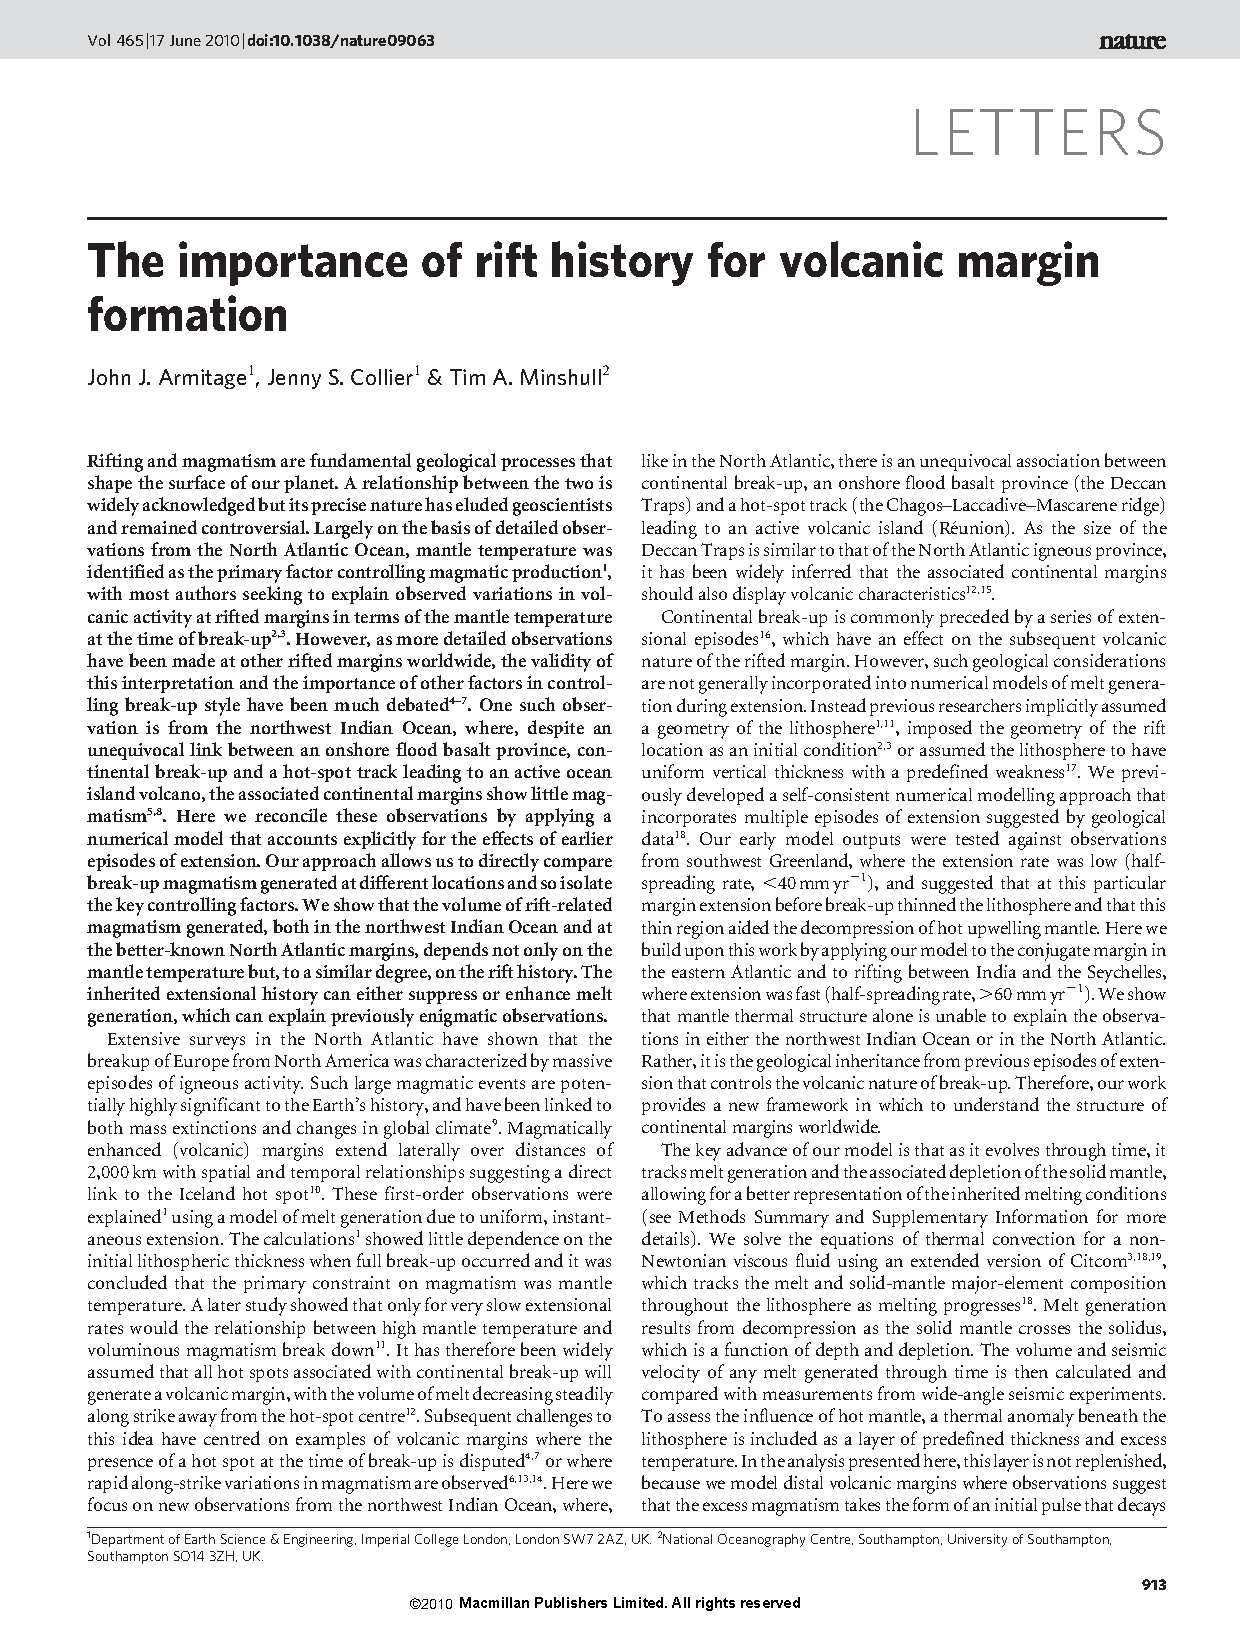
\includepdf[pages=-]{mantle-papers/paper1.pdf}
\includepdf[pages=-]{mantle-papers/paper2.pdf}
\includepdf[pages=-]{mantle-papers/paper3.pdf}
\includepdf[pages=-]{mantle-papers/paper4.pdf}

\chapter{Example Publications Part 2: Surface}

In this final annex I have selected five example publications that explore how surface processes are recorded within the geological record. They also demonstrate the various numerical models I have developed and the collaborations I have formed in order to try and broaden my understanding of the many parts to sedimentology and geomorphology.

\begin{itemize}

\item [1] {\bf Transformation of tectonic and climatic signals from source to sedimentary archive -- Nature Geoscience}

This is where my interest in sedimentology all began. While at Imperial College I got distracted by the work my friends were doing on grain size deposition in alluvial fans. Encouraged by them I developed a novel model that could predict grain sizes deposited as a function of past tectonics and climate (precipitation). This model was used to then demonstrate that change in climate and tectonics leave diagnostically different signatures in the landscape.

\item[2] {\bf Physical stratigraphic model for the Eocene Escanilla sediment routing system: Implications for the uniqueness of sequence stratigraphic architectures -- Journal of Sedimentary Research}

Perhaps my longest title. With funding from the Royal Astronomical Society, I tried to see if I could use the model published in Nature Geosceinces in 2011 to invert the sedimentary record for past climate change. This publication was the result of that work, where the position of key sedimentological markers, such as the gravel front, were used to invert for change in run-off and hence pricipitation.

\item[3] {\bf Deciphering the origin of cyclical gravel front and shoreline progradation and retrogradation in the stratigraphic record -- Basin Research}

Once I had found that my methodology worked for terrestrial deposits I decided to push beyond the shoreline, and explore how the gravel front and shoreline are impacted by climate change and sea-level change. In this study I demonstrate that both a change in run-off and sea level can give similar stratigraphic responses. The difference between the two is recorded in the most proximal regions, suggesting that to fully understand stratigraphy we need complete sections from terrestrial coarse gravel deposits down to marine mud and sand.

\item[4] {\bf  Numerical modelling landscape and sediment flux response to precipitation rate change -- Earth Surface Dynamics}

Landscape evolution models (LEMs) for geological processes tend to treat erosion as either a kinematic wave equation or a diffusive process. In this study I explored the implications of htese two end-member models on the response to change in surface run-off. I found that both models gave similar response, suggesting that it will be difficult to decipher which assumptions are relavent for modelling past landscape change. However, the models both suggest landscape responds more rapidly to a wetting event than a drying event, suggesting that short lived gravel deposition is a signature of increased surface run-off.

\item[5] {\bf Short communication: flow as distributed lines within the landscape -- Earth Surface Dynamics}

While developing the above mentioned study, I noticed that some LEMs where highly resolution dependent. That is to say that the numerical result was a function of the grid resolution. In this final paper I explored the causes of this resolution dependence, and found that how surface water is routed down slope plays a key role in numerical model stability. By routing flow down all slopes I developed a LEM that is not resolution dependent. It remains to be seen if the community will notice.

\end{itemize}

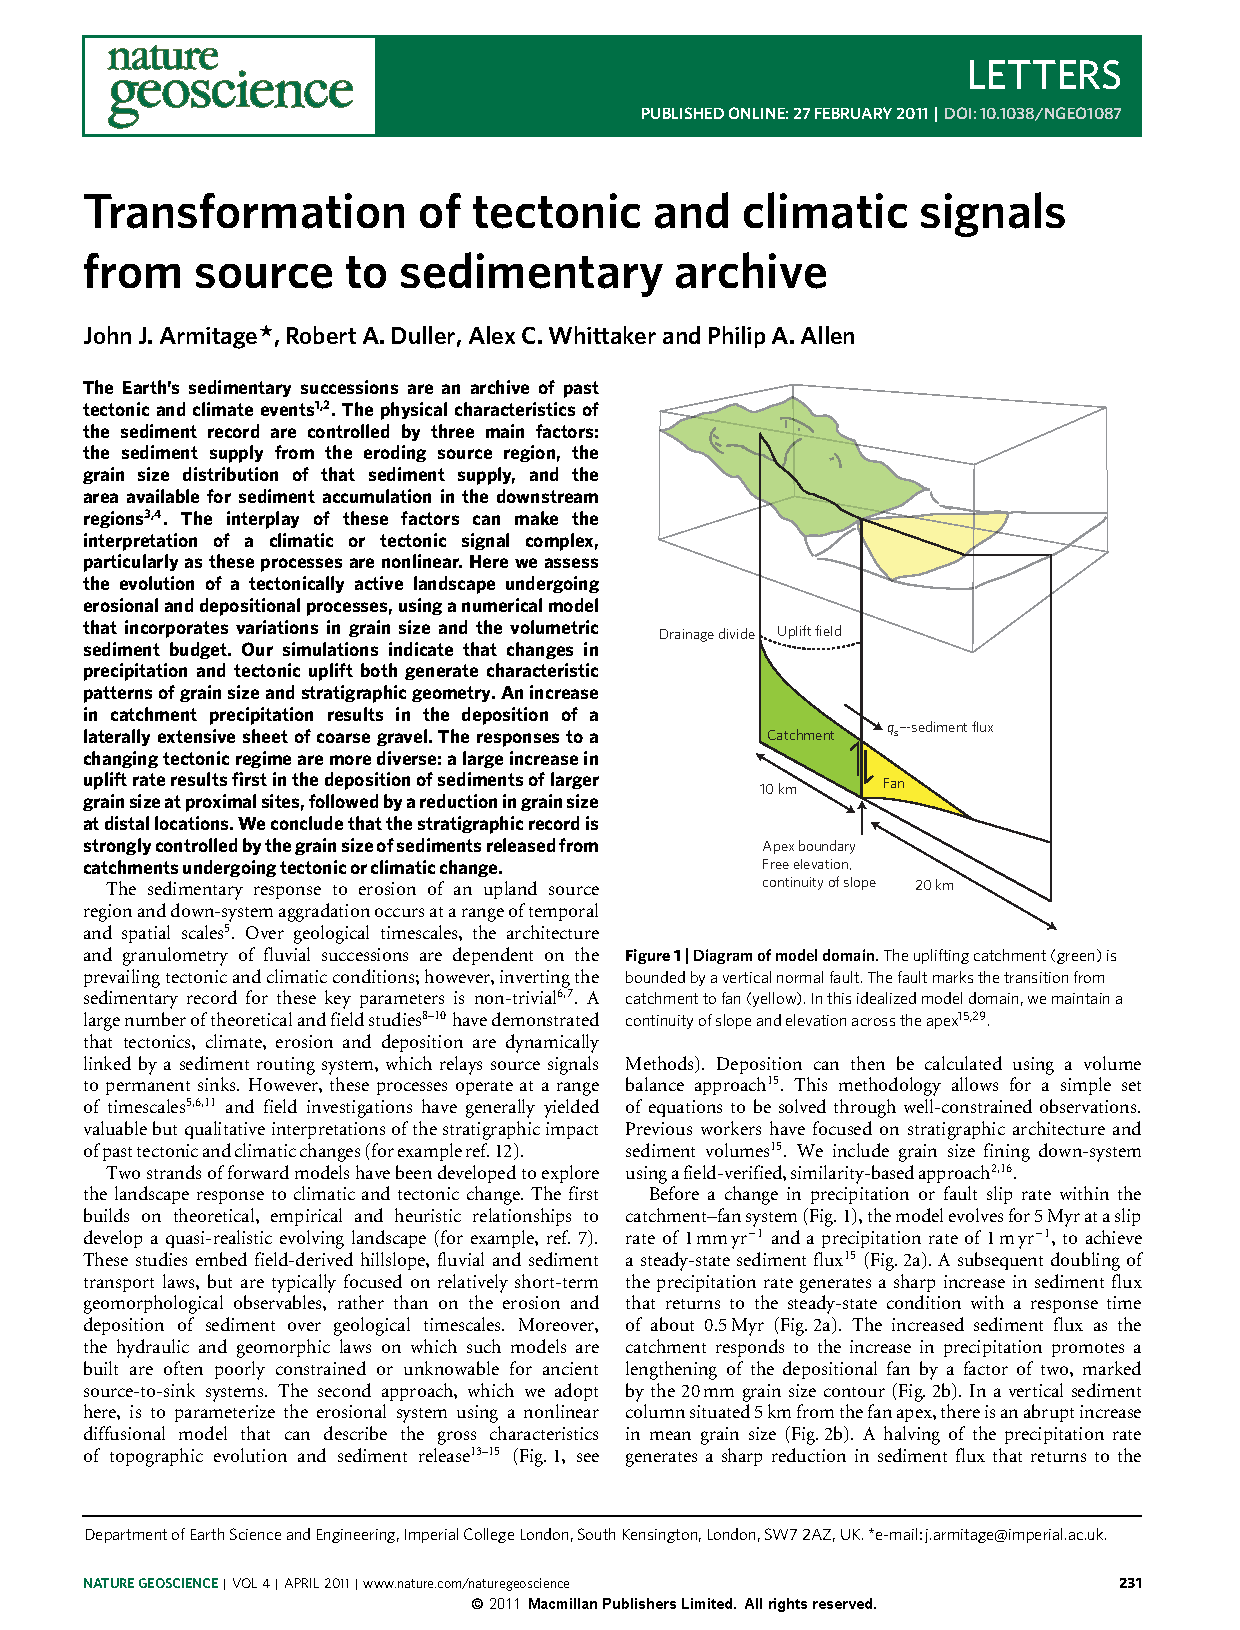
\includepdf[pages=-]{surface-papers/paper1.pdf}
\includepdf[pages=-]{surface-papers/paper2.pdf}
\includepdf[pages=-]{surface-papers/paper3.pdf}
\includepdf[pages=-]{surface-papers/paper4.pdf}
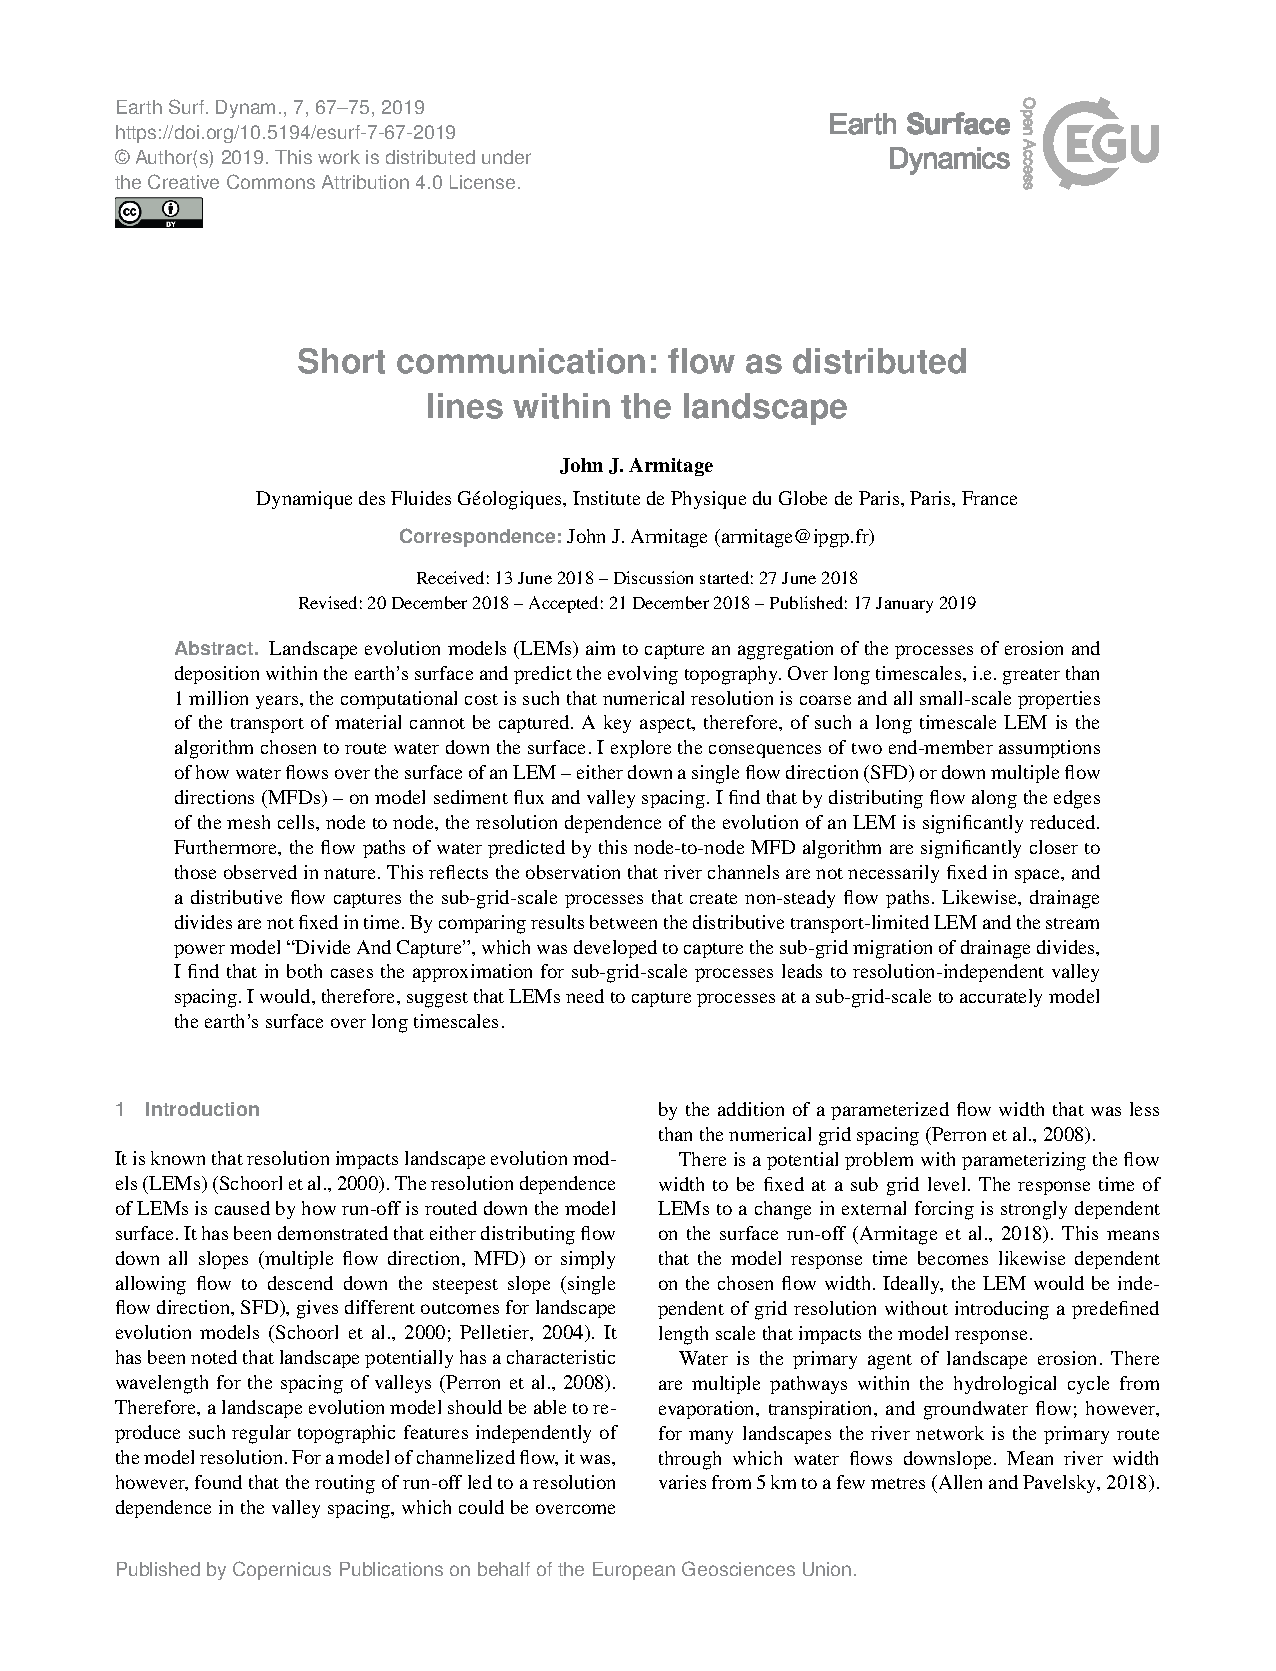
\includepdf[pages=-]{surface-papers/paper5.pdf}

\bibliographystyle{apalike}
\bibliography{../../ref}
}
\end{document}
